\documentclass[a4paper,12pt,twoside,openright]{report}
\usepackage[titletoc]{appendix}
\usepackage{textcomp}
\usepackage[pdftex]{color,graphics}
\usepackage{amssymb}
\usepackage{verbatim}
\usepackage{graphicx}
\usepackage{graphics}
\usepackage{amsmath}
\usepackage{rotating}
\usepackage{setspace}
\usepackage{multirow}
\usepackage{array}
\usepackage{hhline}
\usepackage[labelfont={bf}, margin=0.5cm]{caption}
\usepackage{pdflscape}
\usepackage{subcaption}
\usepackage{caption}
\usepackage{xspace}
\usepackage{float}
\usepackage{placeins}
\usepackage{etoolbox}
\usepackage{xkeyval}[2006/11/18]
\usepackage{datetime}
\usepackage[a4paper,inner=2.5cm,outer=1.5cm,top=2.5cm,bottom=2.5cm,pdftex]{geometry}
\usepackage{emptypage}
\usepackage{hyperref}
\usepackage[export]{adjustbox}

\hypersetup{
	linktocpage,
    colorlinks = true,
	linkcolor = blue,
	citecolor = red
}

\usepackage{fancyhdr}
\fancyfoot{}
\pagestyle{fancy}
\fancyhead[LO]{\leftmark}
\fancyhead[RE]{\rightmark}
\fancyhead[RO,LE]{\thepage}

\renewcommand{\textfraction}{.05}
\renewcommand{\floatpagefraction}{.40}

\newcommand{\gr}{$\gamma$-ray\xspace}
\newcommand{\grs}{$\gamma$-rays\xspace}

\usepackage{lipsum}% just to automatically generate text

\makeatletter
\newcommand\ackname{Acknowledgements}
\if@titlepage
  \newenvironment{acknowledgements}{%
      \titlepage
      \null\vfil
      \@beginparpenalty\@lowpenalty
      \begin{center}%
        \bfseries \ackname
        \@endparpenalty\@M
      \end{center}}%
     {\par\vfil\null\endtitlepage}
\else
  \newenvironment{acknowledgements}{%
      \if@twocolumn
        \section*{\abstractname}%
      \else
        \small
        \begin{center}%
          {\bfseries \ackname\vspace{-.5em}\vspace{\z@}}%
        \end{center}%
        \quotation
      \fi}
      {\if@twocolumn\else\endquotation\fi}
\fi
\makeatother

\newdateformat{monthyeardate}{%
  \monthname[\THEMONTH], \THEYEAR}

%\textheight 24cm
%\textwidth 16.5cm
%\topmargin -1cm
%\oddsidemargin  0cm
%\evensidemargin 0cm
%\flushbottom

%\usepackage{etoolbox}
%\patchcmd{\chapter}{\thispagestyle{plain}}{\thispagestyle{fancy}}{}{}

\setlength{\headheight}{15pt}


\begin{document}


\setcounter{secnumdepth}{3}
\setcounter{tocdepth}{3}

%\doublespace

\pagenumbering{roman}

\begin{titlepage}

\begin{center}

\textbf{\Huge Upgrades to the }

\vspace{3mm}

\textbf{\Huge Fluorescence Detectors of the}

\vspace{3mm}

\textbf{\Huge Pierre Auger Observatory} 

\vspace{3cm}

\includegraphics[width=0.3\textwidth]{pix/UoA_col_vert.png}

\vspace{3cm}


\textbf{\large Tristan William Sudholz} \\
\vspace{0.4cm}
\large School of Physical Sciences \\
\vspace{0.1cm}
\large University of Adelaide

\vspace{1.5cm}
\large This dissertation is submitted for the degree of \\
\vspace{0.2cm}
\textit{\large Doctor of Philosophy}
\vspace{2.5cm}

\monthyeardate\today

\end{center}

\end{titlepage}

\chapter*{Declaration}

I, Tristan William Sudholz, certify that this work contains no material which has been accepted for the award of any other 
degree or diploma in any university or other tertiary institution and, to the best of my knowledge and
belief, contains no material previously published or written by another person, except where due
reference has been made in the text. In addition, I certify that no part of this work will, in the future,
be used in a submission for any other degree or diploma in any university or other tertiary institution 
without the prior approval of the University of Adelaide and where applicable, any partner institution
responsible for the joint-award of this degree.

I give consent to this copy of my thesis, when deposited in the University Library, being made
available for loan and photocopying, subject to the provisions of the Copyright Act 1968.

I also give permission for the digital version of my thesis to be made available on the web, via the
University’s digital research repository, the Library catalogue and also through web search engines,
unless permission has been granted by the University to restrict access for a period of time. 

\vspace{2cm}

\line(1,0){150}

\vspace{1cm}

Tristan William Sudholz
\input{chapters/abstract.tex}
%
\input{chapters/acknowledgements.tex}

\tableofcontents
%\listoffigures
%\listoftables

\chapter*{Nomenclature}

\addcontentsline{toc}{chapter}{Nomenclature}

\begin{tabular}{p{8em} p{30em}}
PAO & Pierre Auger Observatory \\
EAS & Extensive Air Shower \\
NSB & Night Sky Background \\
PE & Photo-electron \\
FD & Fluorescence Detector \\
SD & Surface Detector \\
PMT & Photomultiplier Tube \\
FLT & First Level Trigger
\end{tabular}

% Background Chapters

\chapter*{\centering Introduction \\}\label{Ch:Intro}
\markright{Introduction}
\addcontentsline{toc}{chapter}{Introduction}
\pagenumbering{arabic}

%\begin{itemize}
%\item Define Cosmics Rays.
%\item The origins of the highest energy cosmic-rays still unknown.
%\item First detection by Pierre Auger in 1937 and the current detector looking at theses energies is the Pierre Auger Observatory.
%\item Hybrid experiment containing both surface detectors and fluorescence detectors
%\item Surface detector has nearly 100\% up-time while the fluorescence detectors only have 15\% up-time.
%\item **** Proposal to extend the fluorescence detector up-time. To achieve this will have to operator while the moon is above the horizon. This will increase the level NSB and will have the PMTs run under a reduced gain to compensate. ****
%\item Photomultiplier Tubes are used as pixels within the camera of the fluorescence detectors and  the aim of these thesis is to quantify the characteristics of the PMT under the reduced gain and increased.
%\item Outline a Summary of each chapter.
%\end{itemize}


Cosmic-rays are particles that originate outside of the Earth atmosphere. These particles can be photons, hadronic or leptonic in nature [ref?] and have been measurement over a large range of energies (over 6 decades in energy) since the time of their discovery. A spectrum has been built up over this energy range containing many interesting features with one of the longest running mysteries is what happens at the highest energy.  Since the first detection of extensive air showers by Pierre Auger in 1937 [ref], many different experiments have endeavoured to solve this mystery. The Pierre Auger Observatory [ref] is currently in operation to observe cosmic-rays at top end of the observable energy range.



%In this thesis, when mentioning cosmic-rays I will mean the hadronic component unless specified otherwise. Cosmic-rays have been measurement over a large range of energies (over 6 decades in energy) and it has many interesting features have been observed in this energy spectrum. One of the longest running mysteries is what happens at the highest energy. Since the first detection of extensive air showers by Pierre Auger in 1937 [ref], many different experiments have endeavoured to solve this mystery. The Pierre Auger Observatory [ref] is currently in operation to observe cosmic-rays at the highest energies. 

The Pierre Auger Observatory (PAO) is a hybrid experiment consisting of both surface detectors and fluorescence detectors. PAO is located at Malargue, Mendoza Province, Argentina. There are 1660 surface detectors within an area of 3000 km$^2$ with four fluorescence detector sites surrounding the surface detectors. The fluorescence detectors observe the light emitted from nitrogen molecules that have interacted with charged particles produced from the extensive air shower from the primary particle interacting in the atmosphere. The fluorescence telescopes can view a shower track that is within the Field of View. The surface detectors observe a shower when the secondary particles pass through a detector. The surface detectors only see particles that reach ground level with the fluorescence detectors can observe how the shower develops within the atmosphere. The advantages of the surface detectors is that they has a nearly 100\% operation up-time {ref}, while the fluorescence detectors only 15\% operation up-time [ref]. Also the fluorescence telescopes are used to calibrate the surface detectors.

A proposal in 2015 to extend the fluorescence detector operation up-time was entertained. Extending the FD up-time would be beneficial as the fluorescence detectors image the entire extensive air shower and would increase the number of showers observed through out yearly observation. Currently the FD telescopes gather data during sunless, moonless, cloudless and good weather periods. To achieve an extended operation time, the fluorescence detectors would have to operated while the moon is above the horizon. While the moon is up, this would increased the detected level of background noise (Night Sky Background) and increase the operation load of camera pixels of the Fluorescence detectors. The Fluorescence detectors using Photomultiplier tubes as camera pixels and PMT operations are sensitive to large changes in background noise. To compensate for the large increase in NSB, the PMT gain would be reduced. Current PMT operation is at the minimum of manufacturers specifications and it is wanted to know how the PMTs will act below this minimum specification.


- Need graph of expected variance in ADC$^2$ for the moon above the horizon for different phases.

- Want to increase the duty cycle of FD by measuring EAS under moonlight. Most likely observe under quarter to half moon. This will increased the NSB upto a factor of 10.

- The aim of increasing the duty cycle of FD is too measure more EAS at the highest energy band ($> 10^{19.5}$ eV).

- Need more statistics at highest energy band to complement SD measurements.

The aim of this thesis is to quantify the characteristics of the Photomultiplier Tubes operating under this reduced gain and outline any operation strategies. Outline of each chapter is as follows:

\begin{itemize}
\item  Chapter \ref{Ch:Cosmic-rays}: Cosmic-rays

Does this work as a new line

\item Chapter \ref{Ch:CR_Detection}: Detection of Cosmic-Rays

Add text here

\item Chapter \ref{Ch:PAO}: The Pierre Auger Observatory

Add text here

\item Chapter \ref{Ch:SelectEff} : Extensive Air Shower Selection Efficiency with Increased Night Sky Background 

Add text here

\item Chapter \ref{Ch:PMTCharacter} : Quantifying Characteristics of the Fluorescence Detector Photomultiplier Tubes 

Add text here

\item Chapter \ref{Ch:CompSimPMT} : Computer Simulation of the Fluorescence Detector Photomultiplier Tubes 

Add text here

\item Chapter \ref{Ch:GainVariance} : Measuring Gain Variance of the Fluorescence Detector Photomultiplier Tubes with CalA data 

Add text here

\item Chapter \ref{Ch:GainVariance_Results} : Results of Measuring the Gain Variance of the Fluorescence Detector Photomultiplier Tubes 

Add text here

\item Chapter \ref{Ch:LabPMTshift} : Laboratory Simulation of Fluorescence Detector Shifts

Add text here

\item Chapter \ref{Ch:CloudCuts} : Effectiveness of Cloud Camera Cuts on Data Set

Add text here

%\item Chapter \ref{Ch:Conclusion}: Conclusion 
%
%Future Work


\end{itemize}
\chapter{Cosmic-Rays}\label{Ch:Cosmic-rays}

\section{History of Cosmic-Rays}

First detection of ionizing radiation. 

1785: Coulomb found that 
electroscopes can spontaneously 
discharge by the action of the air 
and not by defective insulation

1835: Faraday confirms the 
observation by Coulomb, with 
better insulation technology

1879: Crookes measures that the 
speed of discharge of an 
electroscope decreased when 
pressure was reduced 

\section{Energy Spectrum and Mass composition}

\section{Production Method and Sources}
\chapter{Detections of Cosmic-Rays}\label{Ch:CR_Detection}

\section{Extensive Air Showers}

Use Earth's atmosphere as an interaction medium.
Primary particle interacts with the molecules in the atmosphere to produce a cascade of secondary particles. This cascade of particles is referred to as an Extensive Air Shower (EAS).
Hadronic primaries can produce pions, muons and other stuff.
Mixture of a hadronic core with an electromagnetic component from the decay of $\pi^{0}$.

Shower profile has particles produced until energy on individual secondary particles drop below the ionization threshold. Therefore the shower will reach a point of maximum particle number then will drop off.

\section{Fluorescence Production}
The charge particles of EAS interact with the nitrogen molecules in the atmosphere. This interaction turns the nitrogen molecule dipole like and when the nitrogen returns to a ground state, a photon is emitted. This emitted photon is termed fluorescence light. Fluorescence light is can be emitted isotropically and typically in the UV band (between 300 and 400 nm). *** Show wavelength profile ***


\section{Atmospheric Effects}



\section{Detectors and History}
\chapter{Pierre Auger Observatory}\label{Ch:PAO}


Science Goals of the Pierre Auger Observatory is to probe the origins and characteristics of cosmic rays above 10$^{17}$ eV and to study the interactions of the most energetic particles observed in nature.

The Pierre Auger Observatory (PAO) is an hybrid detector that is located near Malarg\"ue in the Mendoza Province, Argentina. PAO consists of 1660 Cherenkov water detector spread over 3000 km$^2$  by 24 fluorescence telescopes. 

\begin{figure}[hp]
\centering
\includegraphics[width=0.7\textwidth]{chapters/pix/PAO_equipment_layout_overview.png}
\caption{Image of layout of Pierre Auger Observatory located near Malargue, Argentina.}
\label{fig:PAO_layout}
\includegraphics[width=0.7\textwidth]{chapters/pix/pierre-auger-observatory_tankAndTelescope.jpg}
\caption{Image of one of the fluorescence detector site (background) and one of the surface detectors (foreground).}
\label{fig:PAO_TankAndTelescope}
\end{figure}


\section{Surface Detector}

\begin{figure}
\centering
\includegraphics[width=0.7\textwidth]{chapters/pix/inside_surface_detector.jpg}
\caption{Basic schematic of a surface detector.}
\label{fig:SD_schematic}
\end{figure}

The surface array consists of 1660 water Cherenkov tanks. The majority of tanks are configured with a spacing of 1500 metres while there is a small subset of tanks in front of the fluorescence telescopes at the Coihueco site with spacing of 750 metres. 

The surface array has a duty cycle of nearly 100\% and the maintenance cycle is so that no more then 20 tanks are down at any one time.

\subsection{AugerPrime}

\section{Fluorescence Detector}

\begin{figure}
\centering
\includegraphics[width=0.7\textwidth]{chapters/pix/fluorescence_telescope.png}
\caption{Basic schematic of a fluorescence telescope.}
\label{fig:FD_schematic}
\end{figure}

There are four fluorescence detector site surrounding the surface array. At each fluorescence detector site there are six telescopes covering 180\textdegree \ in azimuth and 30\textdegree \ in elevation. At one site there are three extra telescopes with slightly greater then 90\textdegree \ in azimuth and cover 30\textdegree \ to 60\textdegree \ in elevation.

\subsection{Photomultiplier Tubes}

\section{Communication System and CDAS}

\section{Event Reconstruction}

\subsection{Surface Detector}

\subsection{Fluorescence Detector}

\section{Enhancements and future upgrades}

% Result Chapters

\chapter[The Effects of Increased NSB on the FD Trigger and Reconstruction]{\centering The Effects of \\ Increased Night Sky Background on \\ the Fluorescence Detector's Trigger and Reconstruction \\ }\label{Ch:SelectEff}

\section{Motivation}

The Pierre Auger Observatory has been operational since 2004 and the collaboration  is in the process of rolling out upgrades to improve operations. The upgrade has been name AugerPrime \textbf{(ref)} and is a large project to improve both the Surface Detectors (SD) and the Fluorescence Detectors (FD). The FD portion of AugerPrime involves extending the duty cycle to observe EAS events while the moon is above the horizon. The main purpose of the FD upgrade is to increase the statistics per year for Extensive Air Shower (EAS) events in the highest energy bin ($>$ 10$^{19.5}$ eV). 

In this chapter I used real data and simulations to explore the effects of increasing the Night Sky Background on the collaboration's reconstruction method and trigger efficiency. A real data set was used to evaluate the efficiency of the reconstruction method under different NSB levels by artificially adding extra noise to signal traces. This was a repetition of a study done by M. Unger \textbf{Find ref.} which was used as a starting point and then was expanded on. The expanded work lead to using simulations to evaluate the full trigger and reconstruction efficiency.

\section{Background Information}

\subsection{Current FD Operation}
Currently the Fluorescence Detectors (FDs) are operated under these guidelines: an observation run is organised for nights when the illuminated fraction of the moon less then 70\% and can have a minimum of 3 hours of operation with the moon below the horizon. The FD telescope shutters are then opened when the sun is below -18\textdegree \ of the horizon (beginning of astronomical twilight). The FD shutters remain open while the average variance across the FD camera is less then 100 ADC$^2$/100 ns and the variance of individual PMTs is less then 2000 ADC$^2$/100 ns. The FD shutters at each site will also close if the individual rain sensors are trigger or the measured wind speed is above 50 km/h.  From these guidelines the FD time of operation can be calculated. A calculation performed by the collaboration to estimate the theoretical up time of the FD's was done before 2012 \textbf{(find ref.)} in Table \ref{tab:CFD_Q_F}.
\begin{table}[h]
\centering
\begin{tabular}{c c}
\hline\hline
Theoretical up time & 22\% \\
Loss due to short nights ($<$ 3 hrs) & -2\% \\
Loss due to bad weather or failures & -5\% \\ \hline \hline
Total measurement time & 15\% \\
\hline\hline
\end{tabular}
\caption{Calculation of the FD up-time done by the Collaboration. Bad weather is the inclusion of rain, high wind speeds and lightning strikes in the FDs field of view. Explain Failure - equipment not working.} \label{tab:FD_uptime}
\end{table}
\subsection{NSB and the Moon}
For context, the ADC$^2$/100 ns measured by the FD PMTs at standard operation typically observe Night Sky Background (NSB) with no moon, quarter moon and full moon/twilight are shown in Table \ref{tab:MoonLightADC}. Bad weather is the inclusion of rain, high wind speeds and lightning strikes in the FDs field of view. Failures include any software or hardware issues that prevented any of the FD telescopes from collecting data.
\begin{table}[h]
\centering
\begin{tabular}{c c c}
\hline\hline
Condition & $\sigma^2$ [ADC$^2$/100 ns] & I$_{\mathrm{a}}$ [$\mu$A] \\ \hline\hline
no moon & 25 & 0.5 \\
quarter moon & 250 & 5 \\
full moon/twilight & 2500 & 50 \\ 
\hline\hline
\end{tabular}
\caption{Expected average observed variance in ADC$^2$ and anode current in $\mu$A by the PMTs in the FD telescopes under different NSB conditions. No Moon is the typical conditions that the FD shift is run under.  } \label{tab:MoonLightADC}
\end{table}

- Think about order to put Table 4.2, Figure 4.1 and Figure 4.2

- What to talk about how more observation time we can get while operating under moonlight.

- While under moonlight need to point out the increases in variance that FD's will have to cope with.

\begin{figure}
\centering
\begin{subfigure}[b]{0.45\textwidth}
\includegraphics[width=\textwidth]{chapters/pix/SelEff/IlluminatedMoonFrac_Twilight.JPG}
\caption{}
\end{subfigure}
\hspace*{3mm}
\begin{subfigure}[b]{0.45\textwidth}
\includegraphics[width=\textwidth]{chapters/pix/SelEff/IlluminatedMoon_brightness.JPG}
\caption{}
\end{subfigure}
\caption{\textbf{(a)} Effects on different definitions of twilight. The solid line is the astronomical twilight (sun at least 18\textdegree \ below horizon). The dotted lines represent relaxed definition of twilight with the sun being at 15\textdegree , 12\textdegree \ and 9\textdegree \ below the horizon. \textbf{(b)} Relative brightness of the moon in the nigh sky compared with a full moon as a function of illuminated fraction. Images taken from \textbf{ref{(GAP1996-034)}}. }
\end{figure}

\begin{figure}
\centering
\includegraphics[width=0.8\textwidth]{chapters/pix/SelEff/BGLoop_Variance_crop.jpg}
\caption{Measured NSB variance from the Fluorescence Detectors with different moon illuminated fractions. The moon was 30\textdegree \ above horizon or greater. Image taken from \textbf{ref(Radamir)}.}
\end{figure}

The PMTs used as camera pixels are XP3062 and are operated at a gain of $\sim$ 5 $\times$ 10$^4$ electrons/photo-electron which give the above values in the table. The datasheet \textbf{(find ref.)} for the XP3062 recommend that for good stability anode currents less than 10 $\mu$A be measured. 
  
Later within this thesis I will investigate the effects of lower the gain on the PMTs to reduce the measured anode current. A lower anode current when observing under moonlight would help make sure that the PMT lifespans are not changed by the increased in NSB. A PMT lifetime is measured in the amount of anode current removed in operation. A reduced gain by a factor of ten would theoretical allow the operation of the PMTs while a quarter moon is above the horizon in the same way as the current PMT operation.  

The signal that the FD's observe is AC coupled, which means the mean signal of the NSB is zero. Instead the variance around zero is calculated and is directly proportional to the fluctuations in the NSB. The mean variance of the NSB measured by Auger at Malargue is:
\begin{equation}
\sigma^2_{\mathrm{ADC}} = 25 \ \mathrm{ADC}^2 \ / \ 100 \ \mathrm{ns}
\end{equation}
The ADC is measured in 100 ns increments as that is the digitisation rate within the FD telescopes. The expectation is the three HEAT telescopes which all do the digitisation once per 50 ns.  The mean variance in ADC$^2$ can be converted into photons seen at the aperture by using:
\begin{eqnarray}
\sigma^2_{pe} &=& [\sigma^2_{\mathrm{ADC}}]^{\mathrm{sky}} \ / \ \mathrm{A}^2_{\mathrm{G}} \label{eq:simgaPE} \\
\mathrm{n}_{\mathrm{ph}} &=& \frac{\sigma^2_{pe}}{(1 + \mathrm{V}_{\mathrm{G}})} \label{eq:numPhoton}
\end{eqnarray}
where $\sigma_{pe}$ is the standard deviation of the photo-electron count, n$_{\mathrm{ph}}$ is the photon count and A$_{\mathrm{G}}$ is equal to:
\begin{equation}\label{eq:abs_gain}
\mathrm{A}_{\mathrm{G}} = \frac{1}{\mathrm{C}_{\mathrm{FD}}.\mathrm{f}.\mathrm{Q}}
\end{equation}
where
\begin{itemize}
\item[] A$_{\mathrm{G}}$ is the absolute gain (ADC/photo-electron)
\item[] $\mathrm{C}_{\mathrm{FD}}$ is the FD pixel calibration constant.
\item[] Q is the Quantum efficiency of the PMT turning photons into photo-electrons.
\item[] f is the photon collection efficiency of the telescope optics.
\end{itemize}

/*------ \textbf{Find reference to number below} ------*/

Typical measured values for C$_{\mathrm{FD}}$, Q and f shown in Table \ref{tab:CFD_Q_F}.
\vspace{3mm}
\begin{table}[h]
\begin{center}
\begin{tabular}{|c|c|}
\hline 
C$_{\mathrm{FD}}$ & 4.5 photons/ADC \\
\hline
Q & 0.29 \\
\hline
f & 0.465 \\
\hline
\end{tabular} 
\end{center}
\caption{Typical values for the constants use to calculate A$_{\mathrm{G}}$ which is the absolute gain (ADC/photo-electron). $\mathrm{C}_{\mathrm{FD}}$ is the FD pixel calibration constant, Q is the Quantum efficiency of the PMT turning photons into photo-electrons and f is the photon collection efficiency of the telescope optics.} \label{tab:CFD_Q_F}
\end{table} 

Therefore A$_{\mathrm{G}}$ can be calculated from Eq. \ref{eq:abs_gain} using the values from Table \ref{tab:CFD_Q_F}. If $\sigma^2_{\mathrm{ADC}}$ = 25 ADC$^2$ / 100 ns, through the calculations n$_{\mathrm{ph}}$ = 23 photons / 100 ns. The calculations to work out the standard deviation of the photon count (RMS$_{\mathrm{ph}}$ / 100 ns) from the measured variance in ADC$^2$ is as follows:
\begin{equation}
\mathrm{RMS}_{\mathrm{ph}} = \mathrm{C}_{\mathrm{FD}} \times \sqrt{\mathrm{ADC}^2}
\end{equation}
From all of the equations stated above I have outlined a table showing the expected photon count at the aperture per 100 ns from the measured variance (ADC$^2$ / 100 ns).
\begin{center}
\begin{tabular}{| c | c | c |}
\hline \hline
\textbf{Variance} & \multirow{2}{*}{\textbf{Photons / 100 ns}} & \textbf{RMS} \\
\textbf{(ADC$^2$ / 100 ns)} & & \textbf{(Photons / 100 ns)} \\
\hline \hline
25  & 22.7 & 22.5 \\
\hline
178  & 161.4 & 60 \\
\hline
259  & 226.7 & 71.2 \\
\hline
1000  & 907.0 & 142.3 \\
\hline
\end{tabular}
\end{center}

\subsection{Toy Model of the effect of increased NSB on aperture}

To find a theoretical value for how well a detector will work is to calculate the signal-to-noise ratio. The steps to do this calculation was outline in \ref{P. Sokolsky}. The equation is get the background photo-electron count seen from the night sky is:
\begin{equation}
B \propto \epsilon A b \Delta \Omega \Delta t
\end{equation}
where $\epsilon$ is the optical efficiency of the telescope, $A$ is the mirror area, $b$ is the background light flux and $\Delta\Omega$ is the solid angle of the sky viewed by a single PMT. $B$ calculates the DC signal from the NSB but as the FD is AC coupled this signal is not seen. It is the fluctuations in the NSB that can be interpreted as an EAS signal. The  fluctuations on Noise become:
\begin{equation}
N = \sqrt{B} \propto \sqrt{\epsilon A b \Delta \Omega \Delta t}
\end{equation}



\begin{itemize}
\item Now consider the number of signal photo-electrons:
\begin{equation}
S \propto \frac{\epsilon A n_{e} n_{\gamma} c \Delta t}{4 \pi R^2} e^{-R/\lambda}
\end{equation}
where $n_e$ is the shower size viewed by the PMT, $n_{\gamma}$ is the photon yield per electron for atmospheric scintillation, $R$ is the distance to the shower segment, $c\Delta t$ is the length of the shower segment, and $\lambda$ is the beam attenuation length of light in the atmosphere.
\item The signal-to-noise becomes:
\begin{equation}
\frac{S}{N} = n_e n_{\gamma} c \frac{(1 + cos\theta)}{4 \pi (R sin\theta)^2} \sqrt{\frac{\epsilon A \Delta t}{b \Delta\Omega}} e^{-R/\lambda}
\end{equation}
\item $\theta$ is the viewing angle of the EAS.
\end{itemize}

\begin{itemize}
\item Calculating the Rayleigh Attenuation Length:
\begin{equation}
x_R = 2974 \left(\frac{\lambda}{400 \ nm} \right)^4 g/cm^2
\end{equation}
\item We want the light path $\Delta$X$_P$ also in g/cm$^2$ so the attenuation factor will be:
\begin{equation}
exp(-X / x_R )
\end{equation}
\item Convert R$_P$ to $\Delta$X$_P$:
\begin{eqnarray}
h &=& R_P sin15^{\circ} \\
\Delta X_{vertical} &=& 860 - 860exp(-h/7500)
\end{eqnarray}
\item Light path in grammage:
\begin{equation}
\Delta X_P = \Delta X_{vertical} / cos75^{\circ}
\end{equation}
\end{itemize}

\begin{figure}
\centering
\includegraphics[height=0.45\textheight]{chapters/pix/SelEff/ShowerPlane_and_Detector.png}
\caption{Diagram showing the parameters used. Also show how they relate to the plane of the shower axis and to the position of the detector.}
\end{figure}

\begin{figure}
\centering
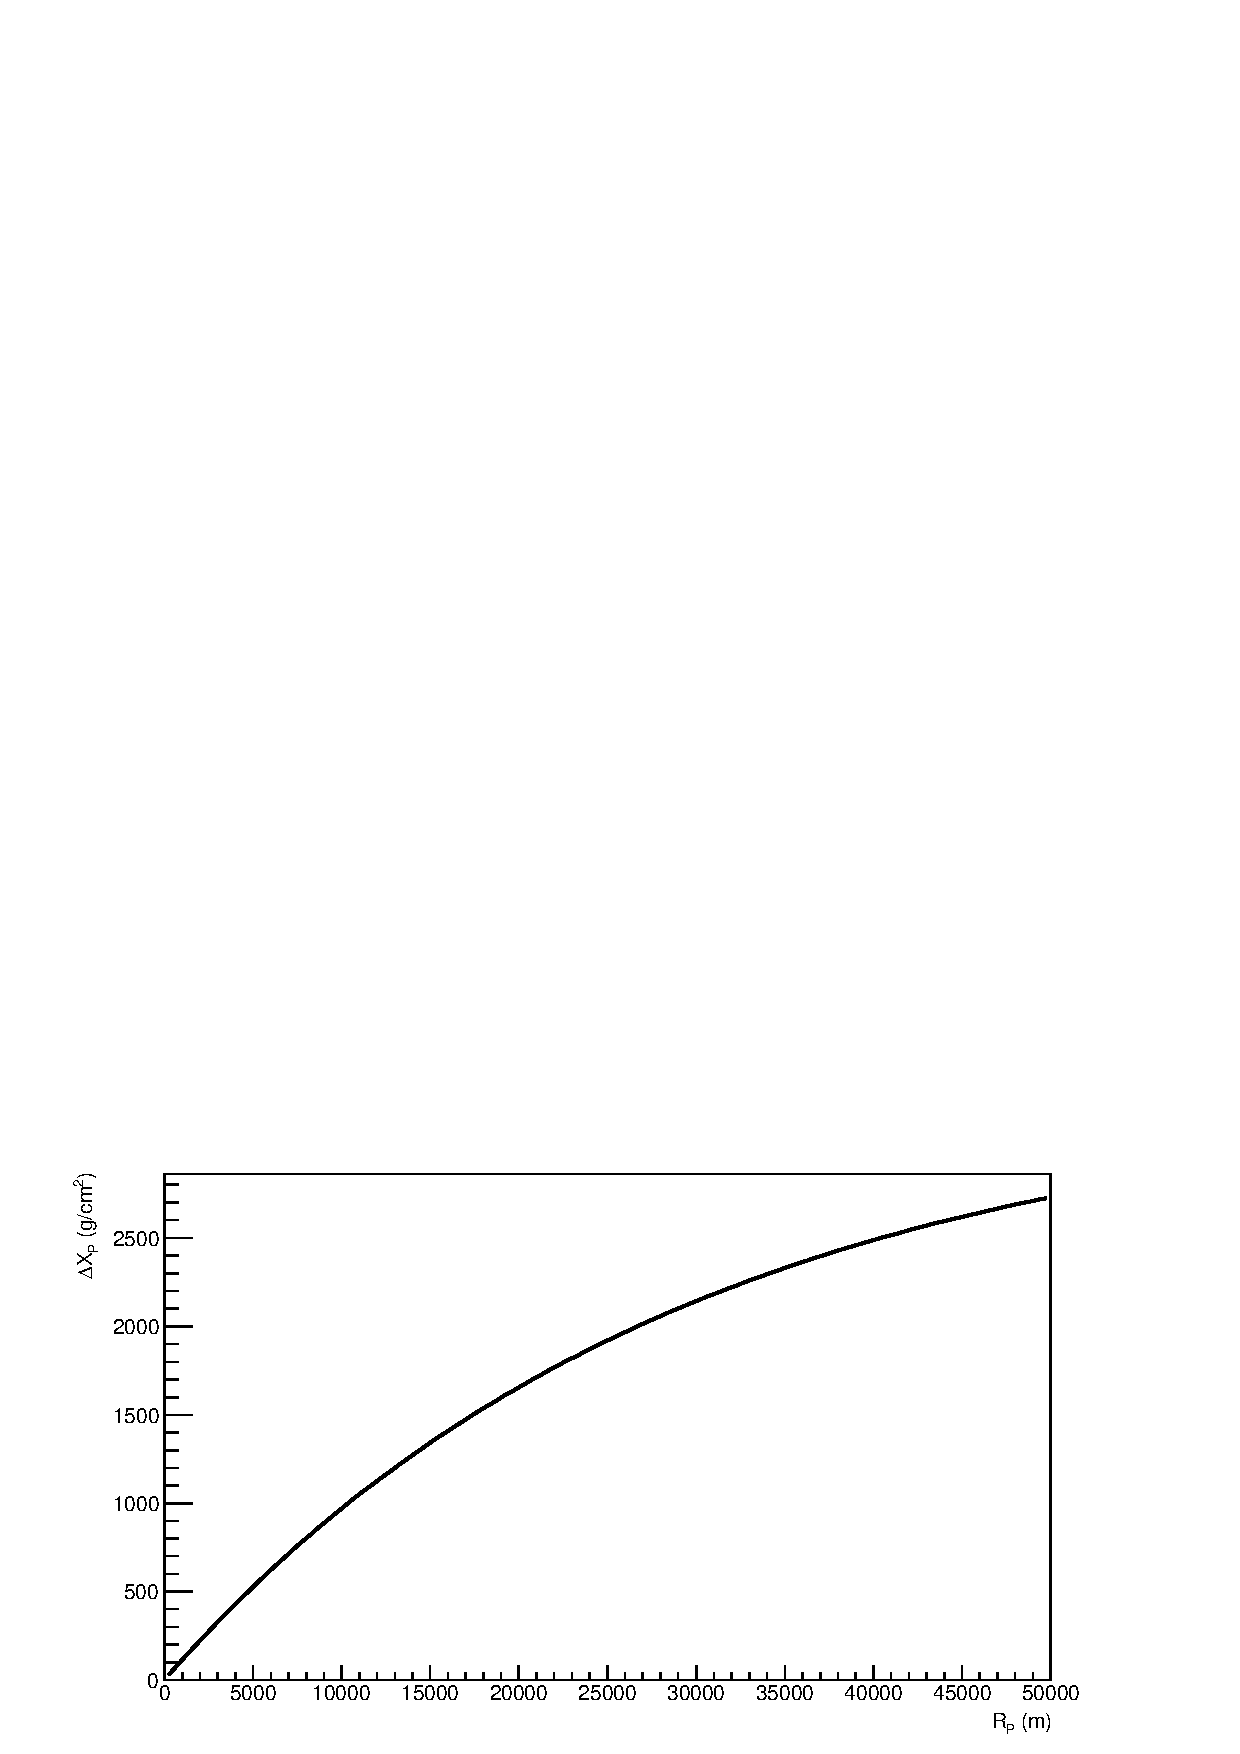
\includegraphics[width=\textwidth]{chapters/graphs/SelectionEff/XpVsRp.pdf}
\caption{How the relationship between the distance to the shower axis and grammage along the path. In this case the distance to the shower axis is denoted R$_P$ and the grammage is denoted $\Delta$X$_P$. The angle of the shower is 15$^{\circ}$}
\end{figure}

\begin{figure}
\centering
\includegraphics[width=\textwidth]{chapters/graphs/SelectionEff/RangeIncreaseVsRangeStand_Xp.pdf}
\caption{The image of how a detector measure the Signal-to-Noise ratio the NSB at the Standard value and Increased by a factor of 10 as a function of distance. The dashed black line denotes the distances where the Signal-to-Noise ratio is the same. The solid black line denotes where the distances are equal.}
\includegraphics[width=\textwidth]{chapters/graphs/SelectionEff/RatioAreaVsDistance_Xp.pdf}
\caption{The image shows how the ratio of the detector viewing area changes with increasing the NSB by a factor of 10 as a function of distance from the detector. The solid black line denotes where the Signal-to-Noise ratio is the same.}
\end{figure}

\begin{figure}
\centering
\begin{subfigure}[b]{0.45\textwidth}
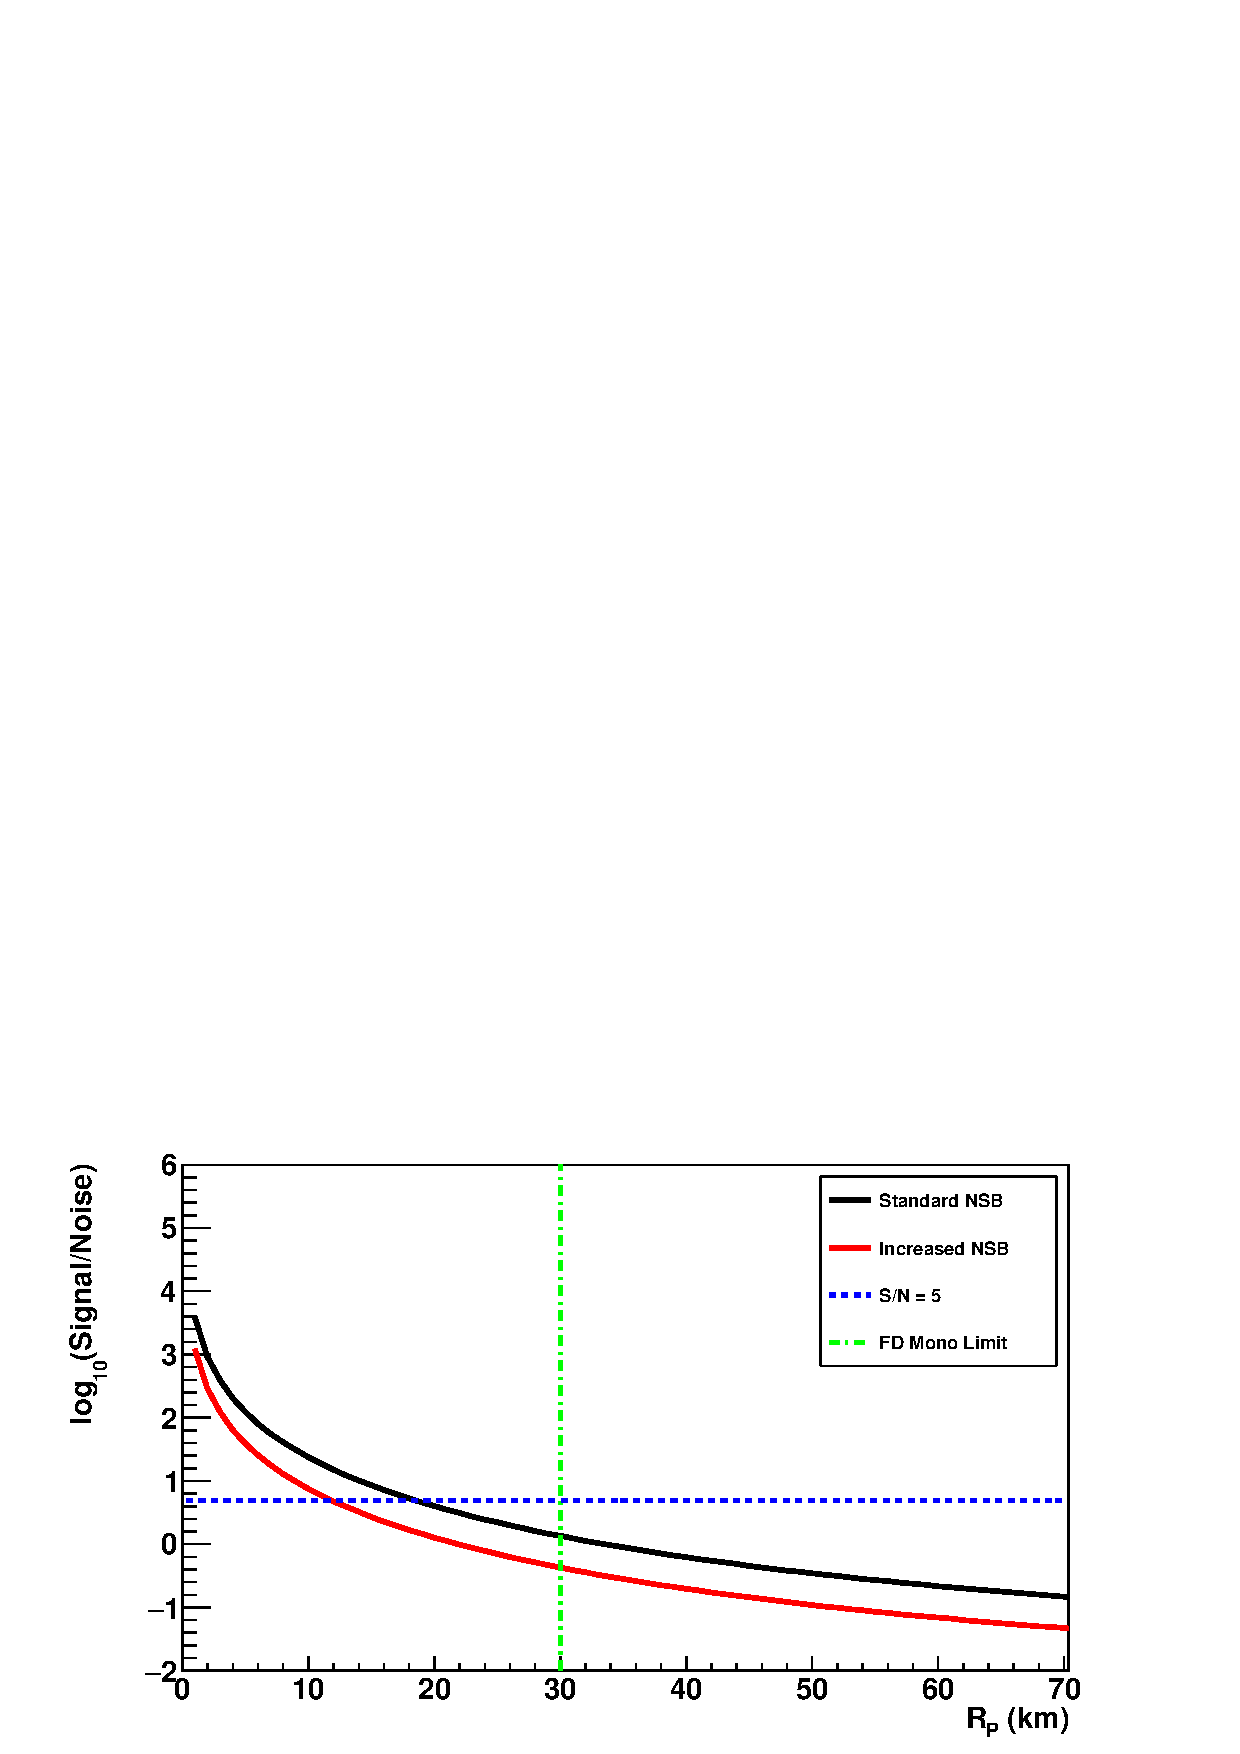
\includegraphics[width=\textwidth]{chapters/graphs/SelectionEff/SignalToNoiseVsDistance_E1e18eV.pdf}
\caption{E = 1 $\times$ 10$^{18}$ eV}
\end{subfigure}
\hspace{3mm}
\begin{subfigure}[b]{0.45\textwidth}
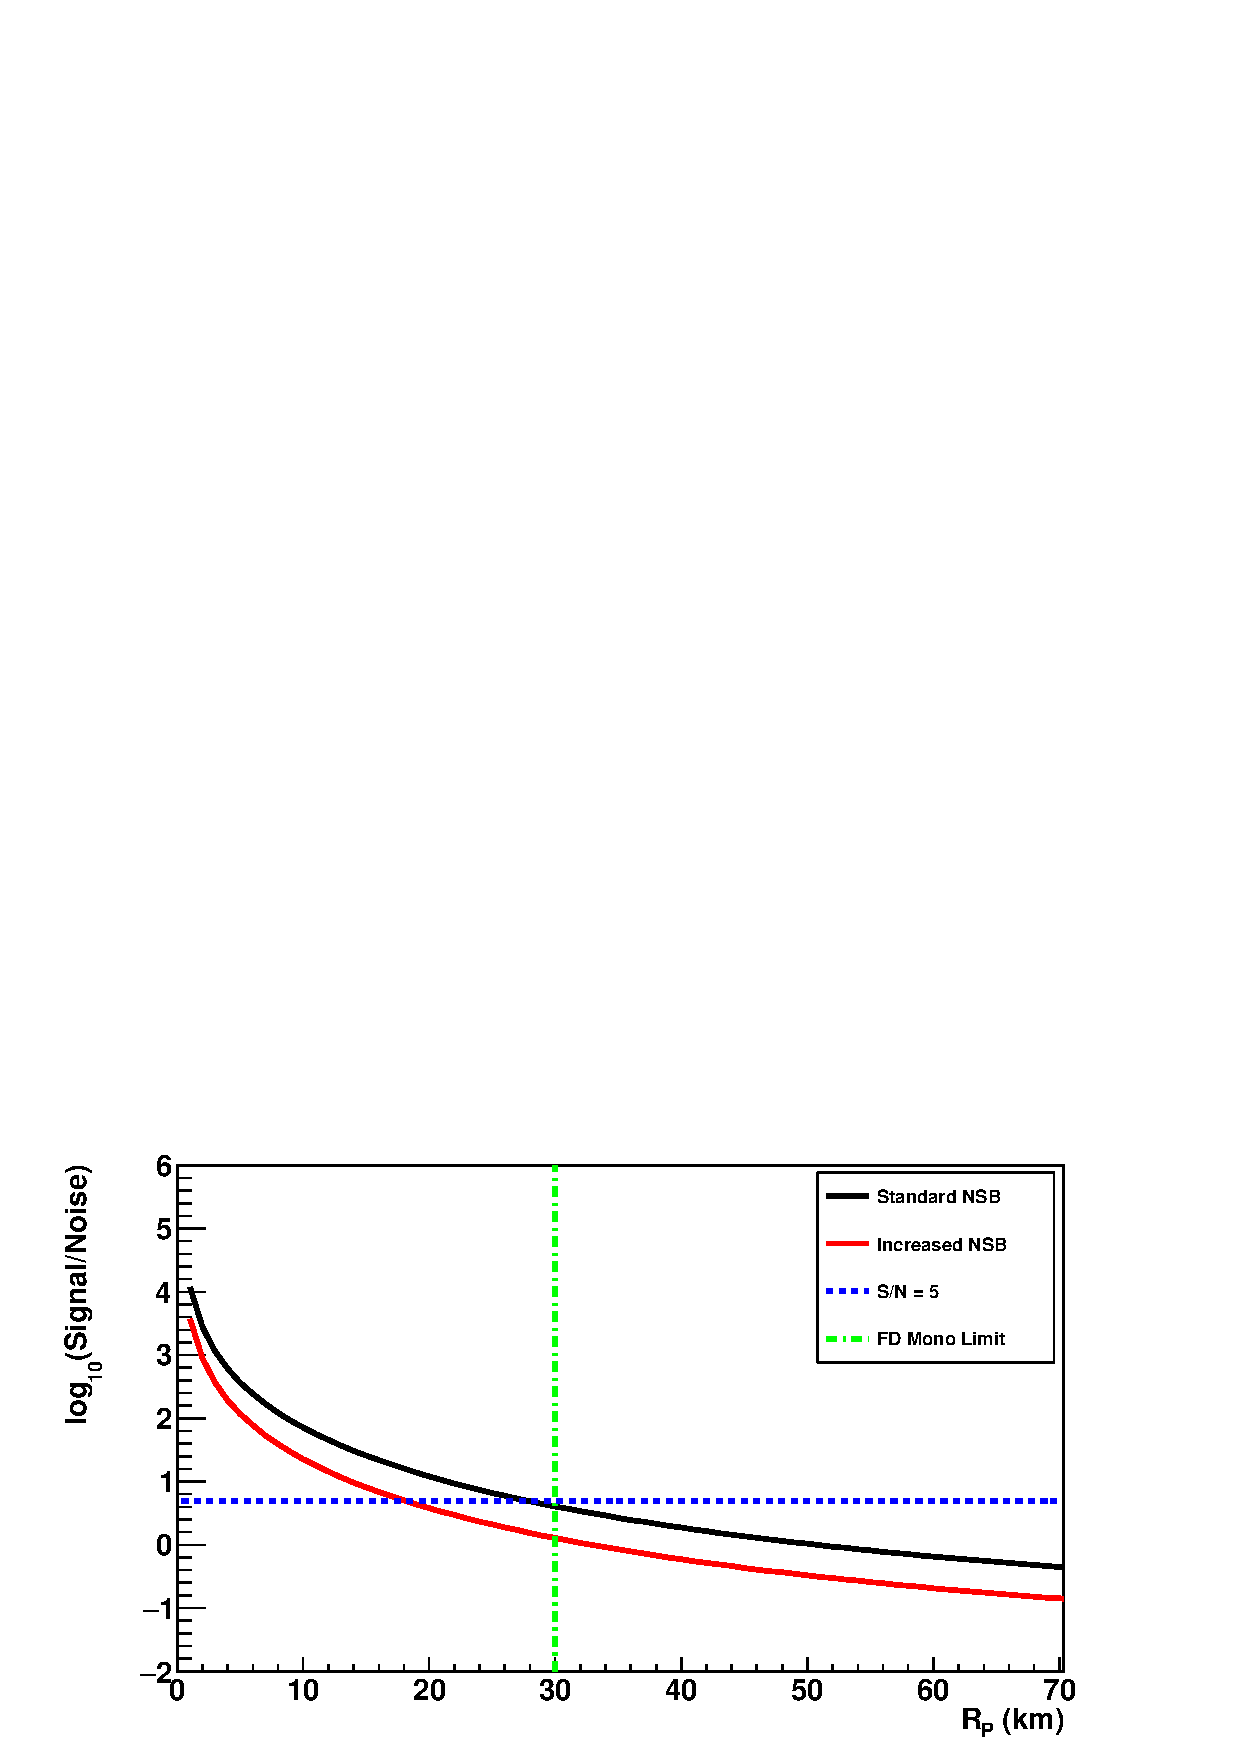
\includegraphics[width=\textwidth]{chapters/graphs/SelectionEff/SignalToNoiseVsDistance_E3e18eV.pdf}
\caption{E = 3 $\times$ 10$^{18}$ eV}
\end{subfigure}
\vspace{3mm}
\begin{subfigure}[b]{0.45\textwidth}
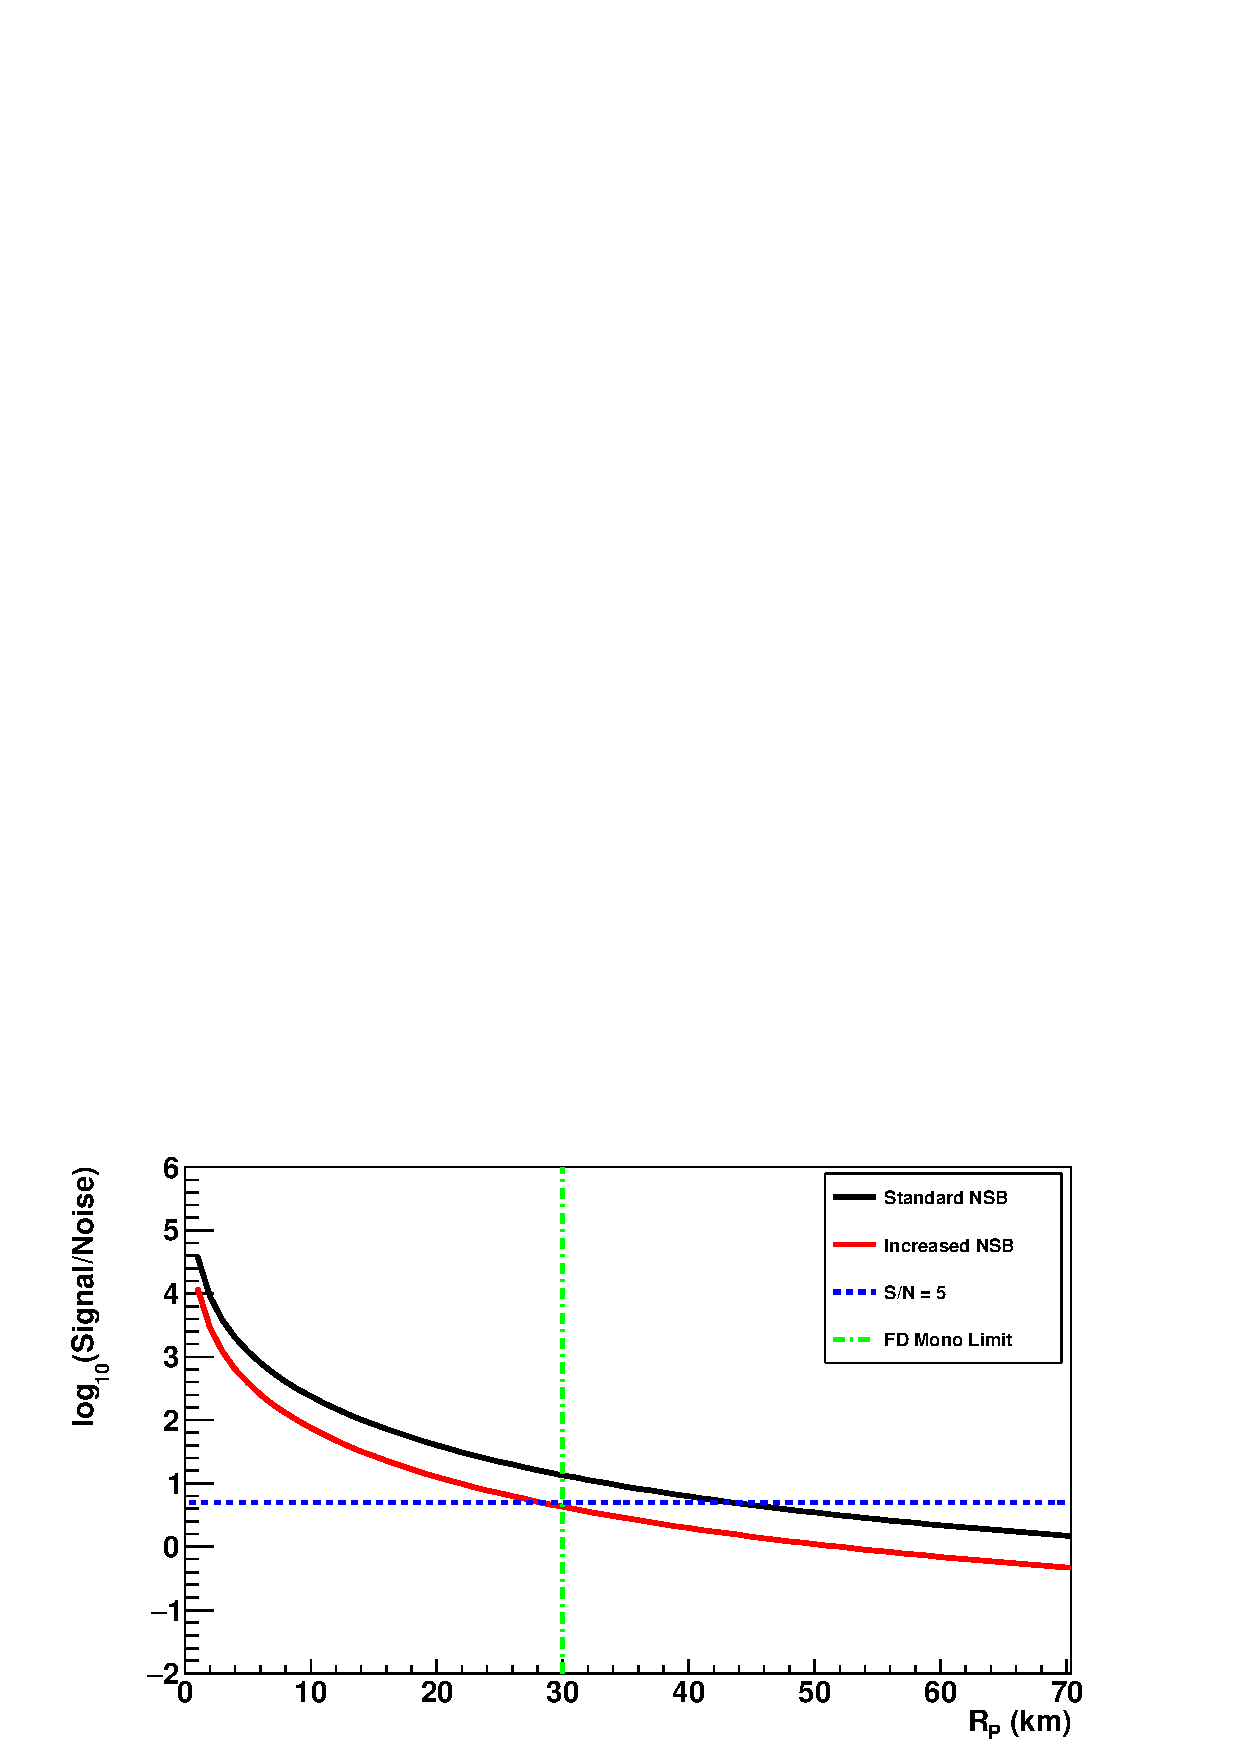
\includegraphics[width=\textwidth]{chapters/graphs/SelectionEff/SignalToNoiseVsDistance_E1e19eV.pdf}
\caption{E = 1 $\times$ 10$^{19}$ eV}
\end{subfigure}
\hspace{3mm}
\begin{subfigure}[b]{0.45\textwidth}
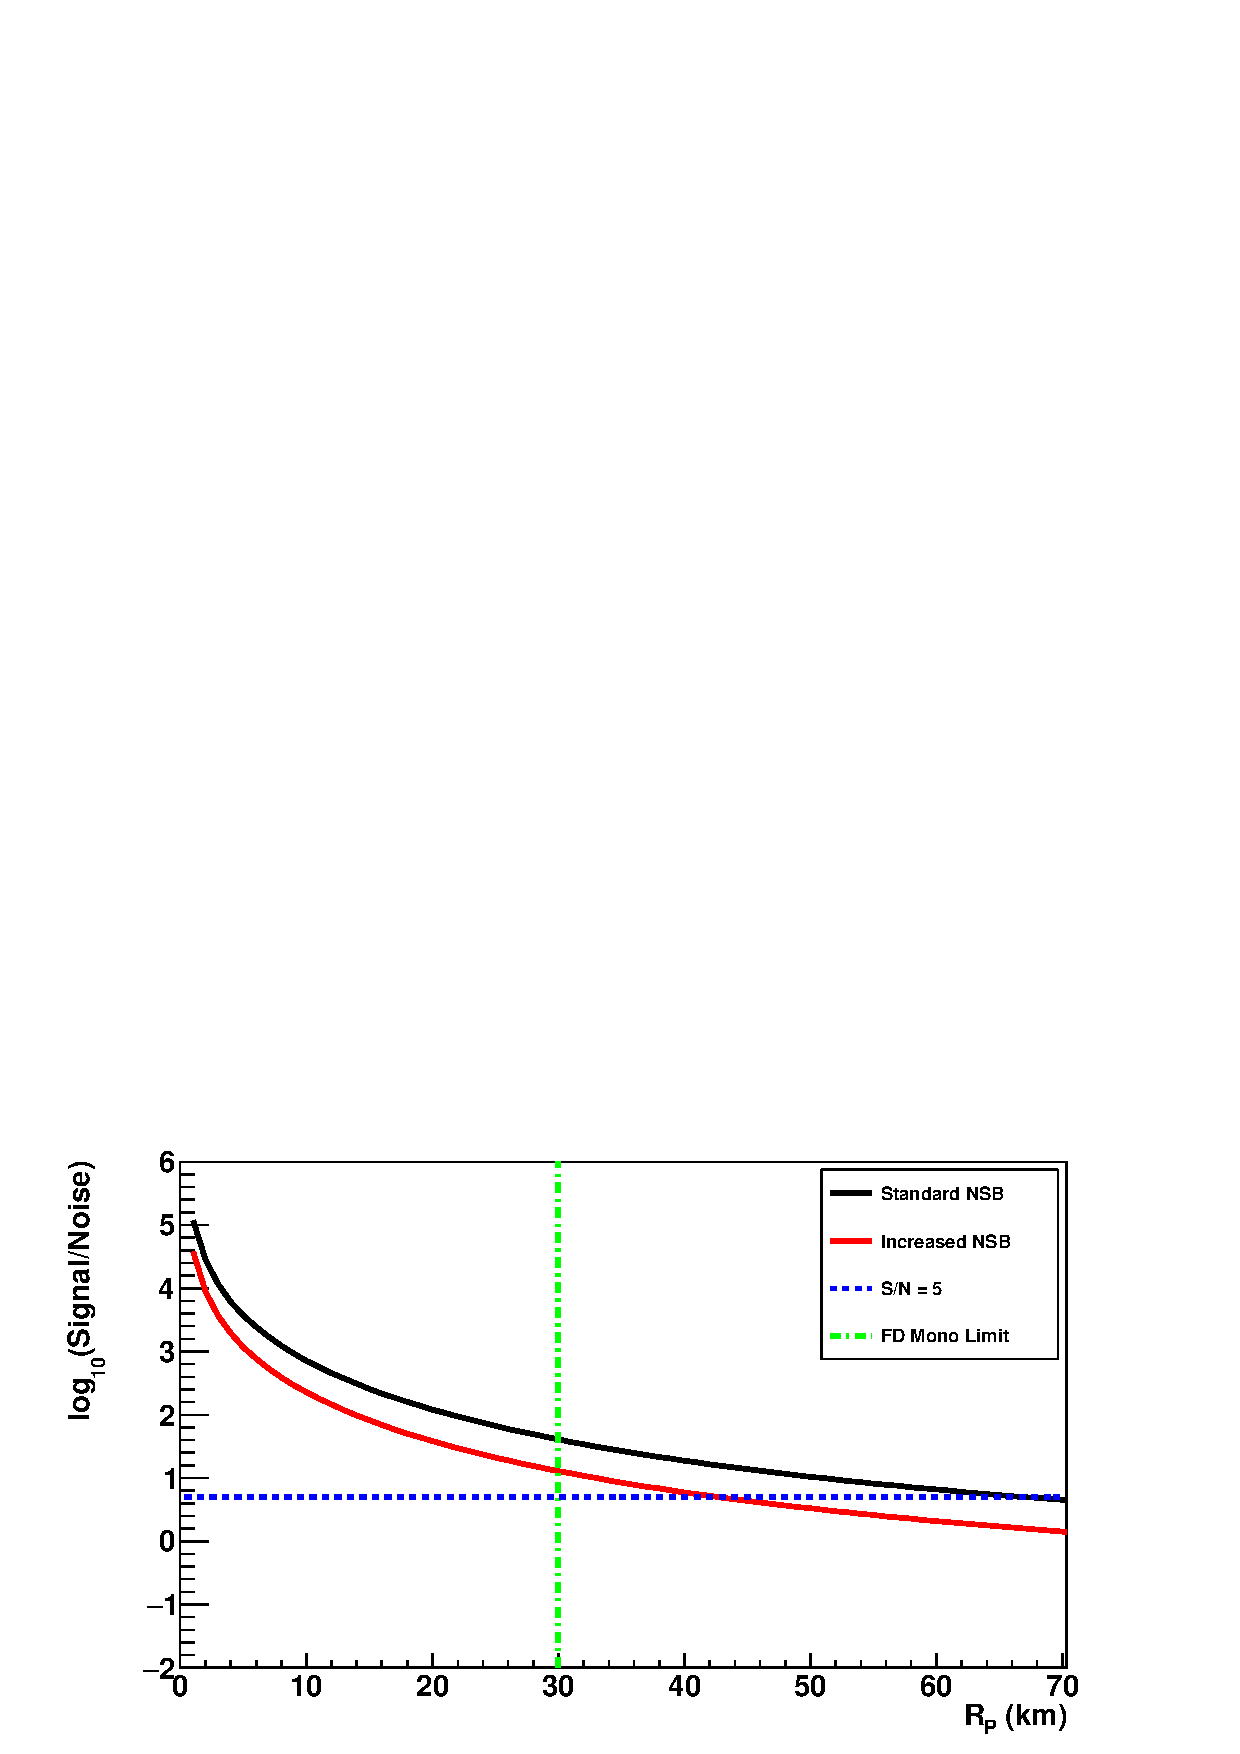
\includegraphics[width=\textwidth]{chapters/graphs/SelectionEff/SignalToNoiseVsDistance_E3e19eV.pdf}
\caption{E = 3 $\times$ 10$^{19}$ eV}
\end{subfigure}
\caption{Using values for the equation to calculate the Signal-to-Noise ratio from specific values for the FD, NSB and conversion's from shower energy to photons to photo-electrons. }
\end{figure}

\section{Increasing NSB in Real Data to evaluate Reconstruction Efficiency}


I investigated evaluating increasing the NSB by different factors on event reconstruction seen by the FD's through two different methods. In this section I will be discussing the method used to evaluate the effects of increasing the NSB on the reconstruction efficiency with the use of real data. The method involved using the raw signal traces from fluorescence telescope EAS shower events that would passed reconstruction and quality cuts and adding addition variance in ADC$^2$ equivalent to an increased NSB from moonlight to the FD pixel signal traces.  The shower events are then reconstructed and passed through the same quality cuts. 

This a repetition of a similar method that M. Unger had preformed in \textbf{2012}. \textbf{Also need to refer to the study done by Brue and Andrew Smith around 1999}. Adding artificial noise to the signal traces was used as an initial proof of concept that EAS showers could still be reconstructed with our current software package. I repeated this study to have a known base-line to work from and have the ability to perform a deeper analysis to understand any underlying mechanics. 

\subsection{Method}
 The Efficiency was calculated with the equation used:
\begin{equation}
\mathrm{Efficiency} = \mathrm{N}^{'}_{\mathrm{Select}} \ / \ \mathrm{N}^0_{\mathrm{Select}}
\end{equation}
where $\mathrm{N}^{0}_{\mathrm{Select}}$ is the number of selected events at the standard NSB level and $\mathrm{N}^{'}_{\mathrm{Select}}$ is the number of selected events at the increased NSB
level. 

After the Efficiency was calculated the bias and resolution for Xmax and energy was determined. For real data, the bias is the relative change in the mean of the distributions at increased NSB to the mean of the distributions at standard NSB, both after reconstruction and selection cuts. The bias calculations for real data become:
\begin{eqnarray}
\Delta \mathrm{E}_{\mathrm{Data}} &=& \frac{\mathrm{E}_{\mathrm{IncreasedNSB}} - \mathrm{E}_{\mathrm{StandardNSB}}}{\mathrm{E}_{\mathrm{StandardNSB}}} \label{eq:energybias_data} \\
\Delta \mathrm{Xmax}_{\mathrm{Data}} &=& \mathrm{Xmax}_{\mathrm{IncreasedNSB}} - \mathrm{Xmax}_{\mathrm{StandardNSB}}\label{eq:xmaxbias_data}
\end{eqnarray} 
For simulated data the bias is the relative change in the mean of the distributions after the full simulation by EAS events going through an atmosphere with a specified NSB photon field, the FD telescopes optics, trigger, reconstruction and selection cuts compared with Monte-Carlo truth.
\begin{eqnarray}
\Delta \mathrm{E}_{\mathrm{Sim}} &=& \frac{\mathrm{E}_{\mathrm{recon}} - \mathrm{E}_{\mathrm{true}}}{\mathrm{E}_{\mathrm{true}}}  \label{eq:energybias_sim} \\
\Delta \mathrm{Xmax}_{\mathrm{Sim}} &=& \mathrm{Xmax}_{\mathrm{recon}} - \mathrm{Xmax}_{\mathrm{true}} \label{eq:xmaxbias_sim}
\end{eqnarray}
 
 
The energy and Xmax resolution is calculated via:
\begin{eqnarray}
\sigma_{\mathrm{res}} &=& \left( \frac{1}{\mathrm{N}} \sum \frac{1}{\sigma^2_i} \right)^{1/2}
\end{eqnarray}

To further evaluate the effects of increasing the NSB on the quality of the reconstructed EAS data, I look at the resolution and bias of both the reconstructed energy and reconstructed Xmax. A quick reminder that Xmax is the measurement of the brightest part of the shower relating to the maximum number of particles produced. For the smearing method the energy and Xmax bias is comparing to the measured data taken at standard NSB levels to the reconstructed with the increased NSB levels. For the simulations the energy and Xmax bias can be calculated using the true energy and Xmax values used to generate each EAS profile.

The trend of the energy resolution for both methods is that as the energy of the EAS event increases the bias decreases. This was expected as the energy of the shower increases the brighter and longer the track that is observed. A brighter and longer track allows for a better reconstruction.

\subsection{Results}
\begin{figure}
\centering
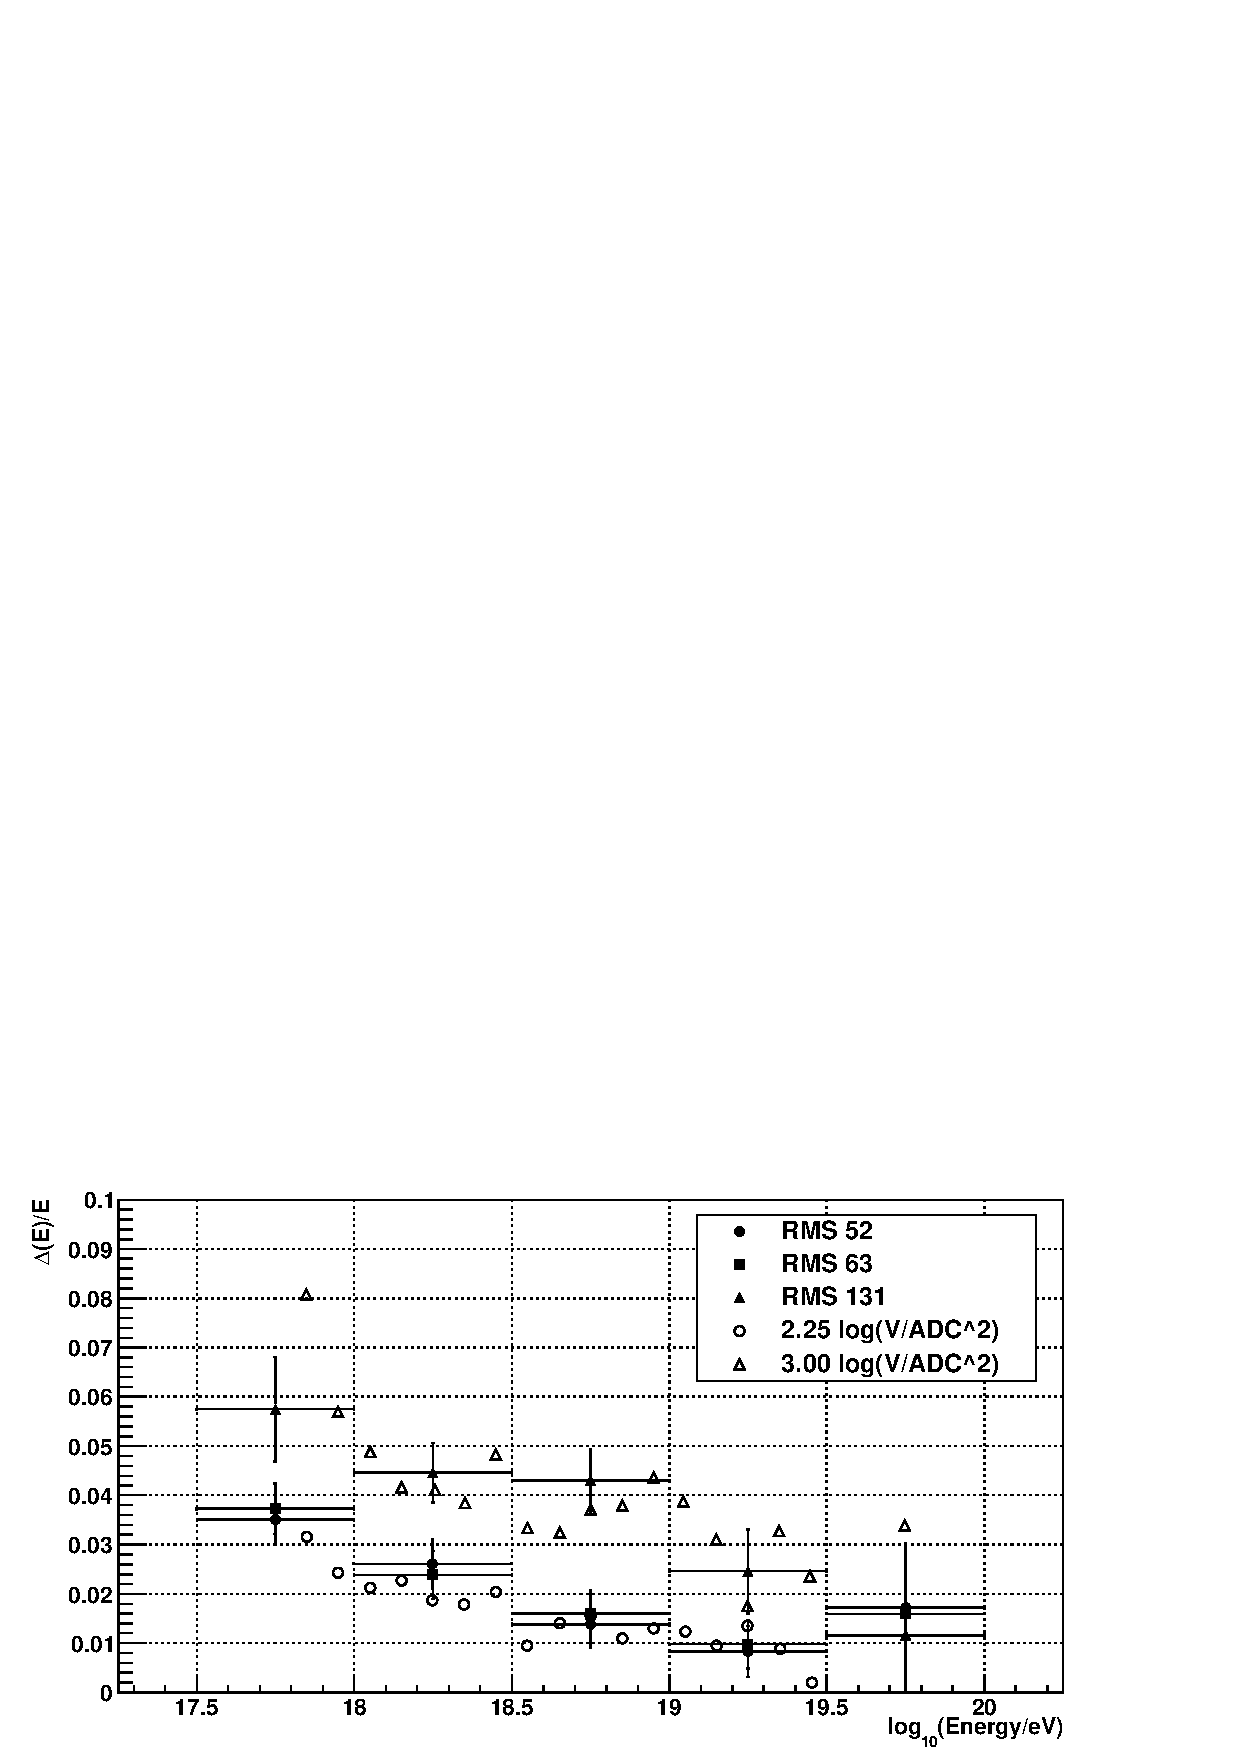
\includegraphics[width=\textwidth]{chapters/graphs/SelectionEff/Smearing_RealData_EnergyBias.pdf}
\caption{Energy Bias using Smearing Method.}
\vspace{3mm}
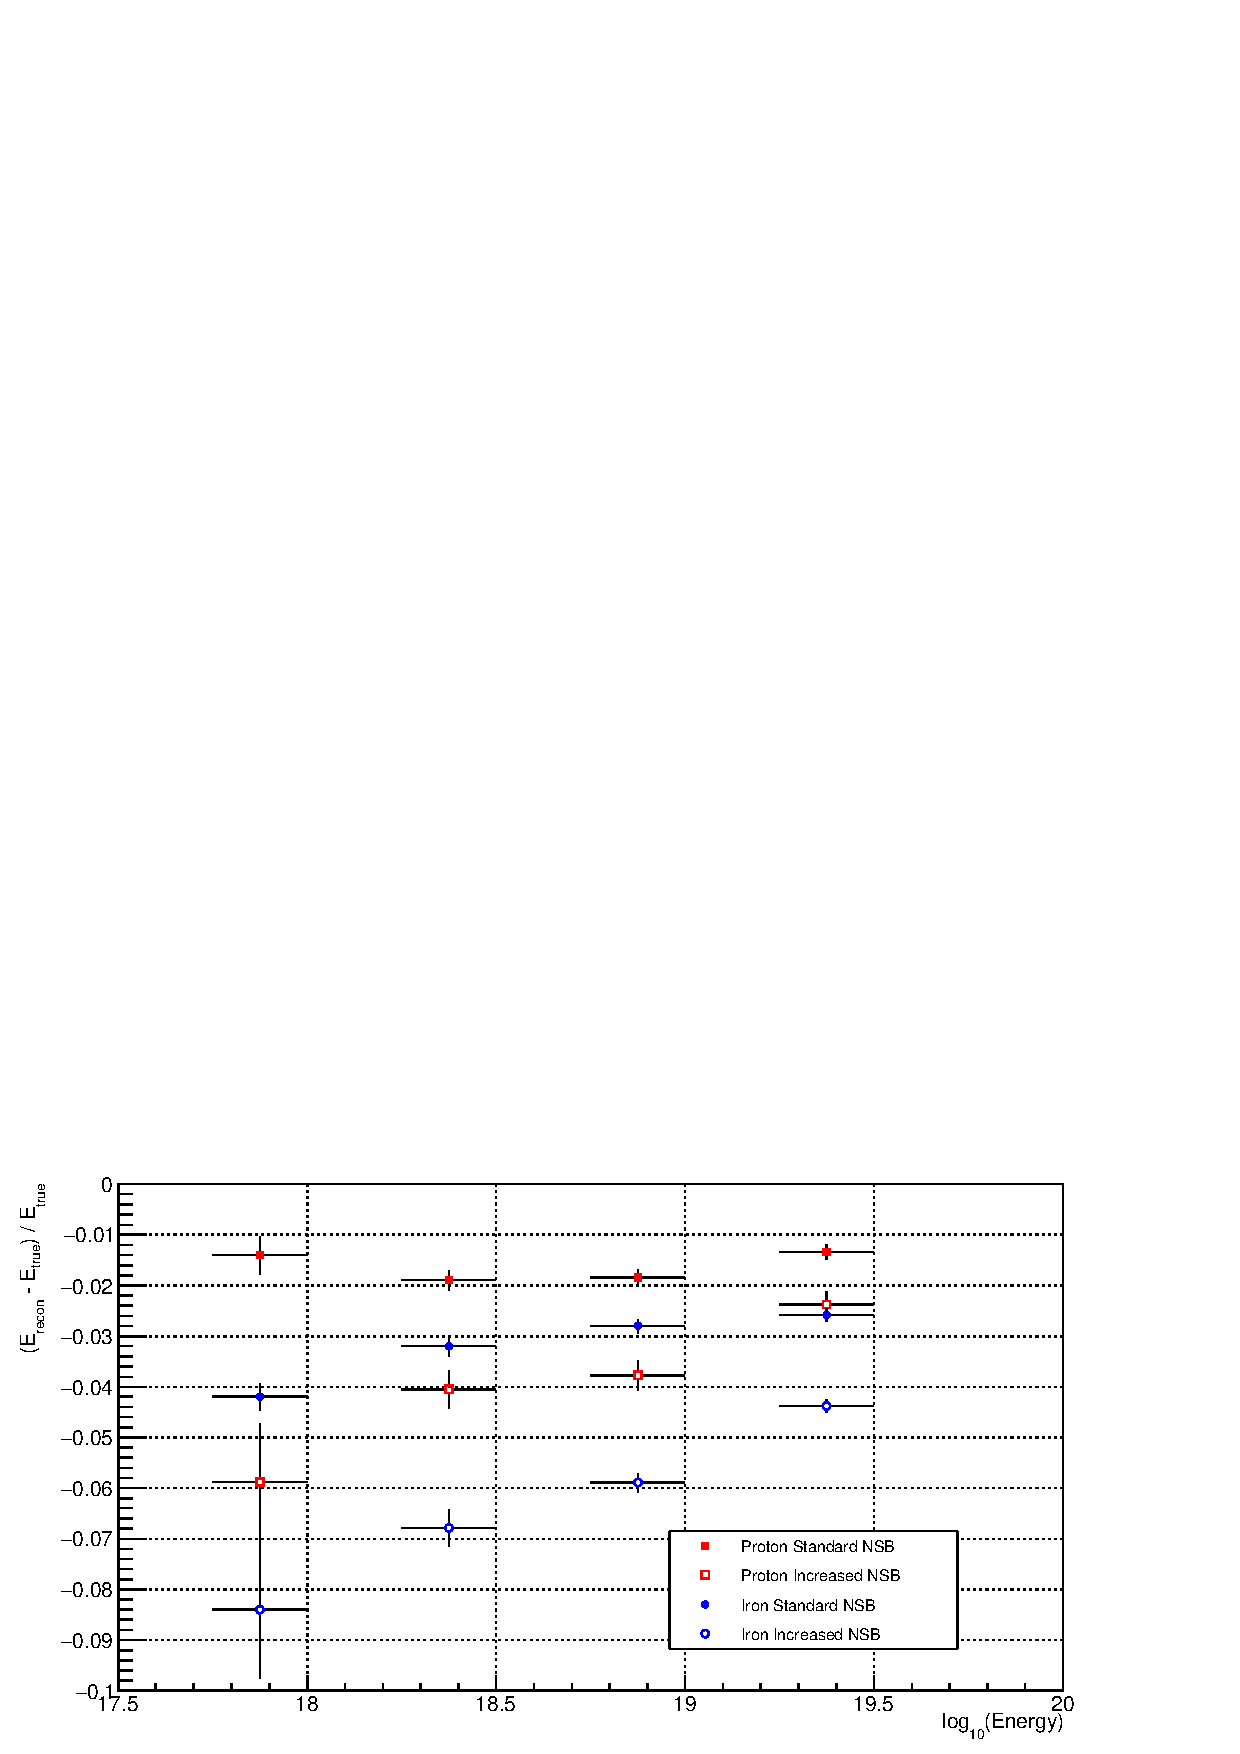
\includegraphics[width=\textwidth]{chapters/graphs/SelectionEff/Simulation_ProtonIron_EnergyBias.pdf}
\caption{Energy Bias using simulated data.}
\end{figure}

\begin{figure}
\centering
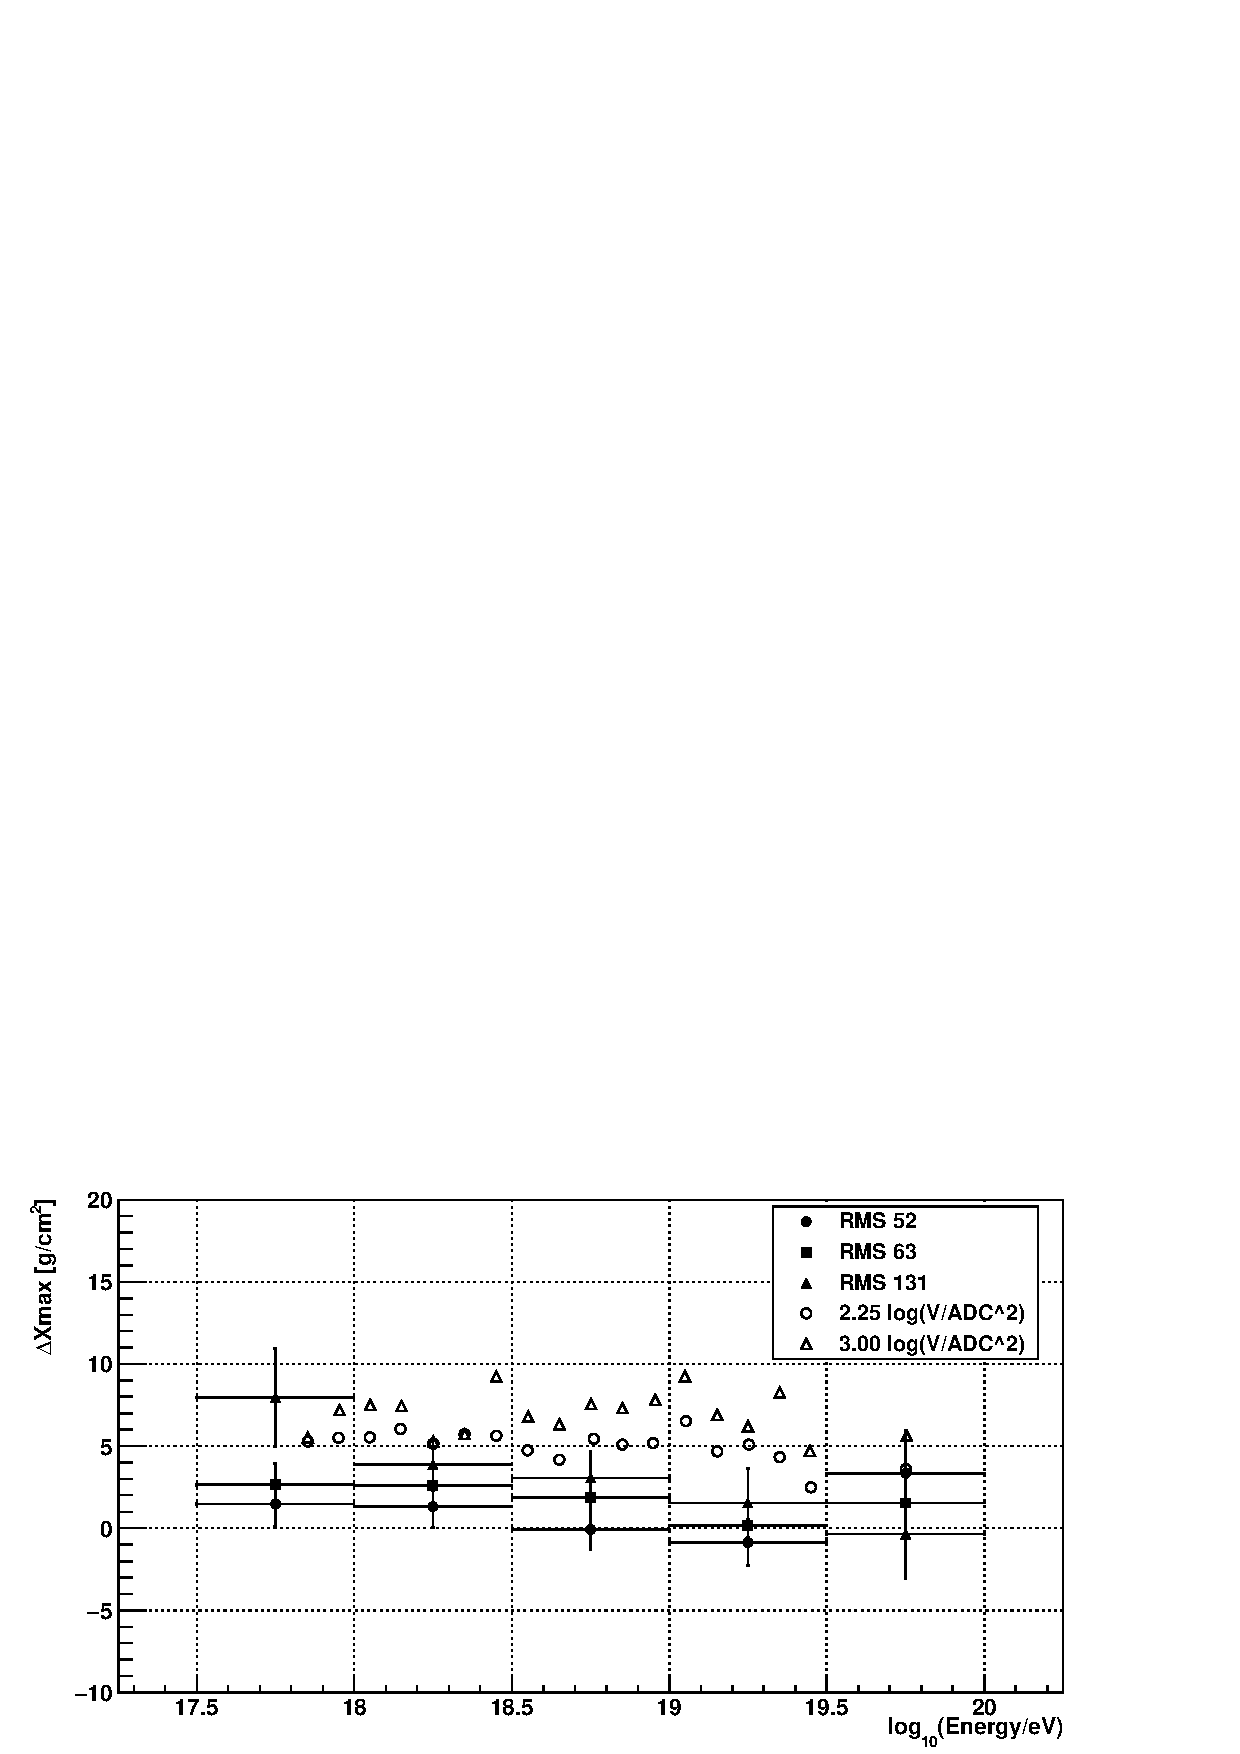
\includegraphics[width=\textwidth]{chapters/graphs/SelectionEff/Smearing_RealData_XmaxBias.pdf}
\caption{Xmax Bias using Smearing Method.}
\vspace{3mm}
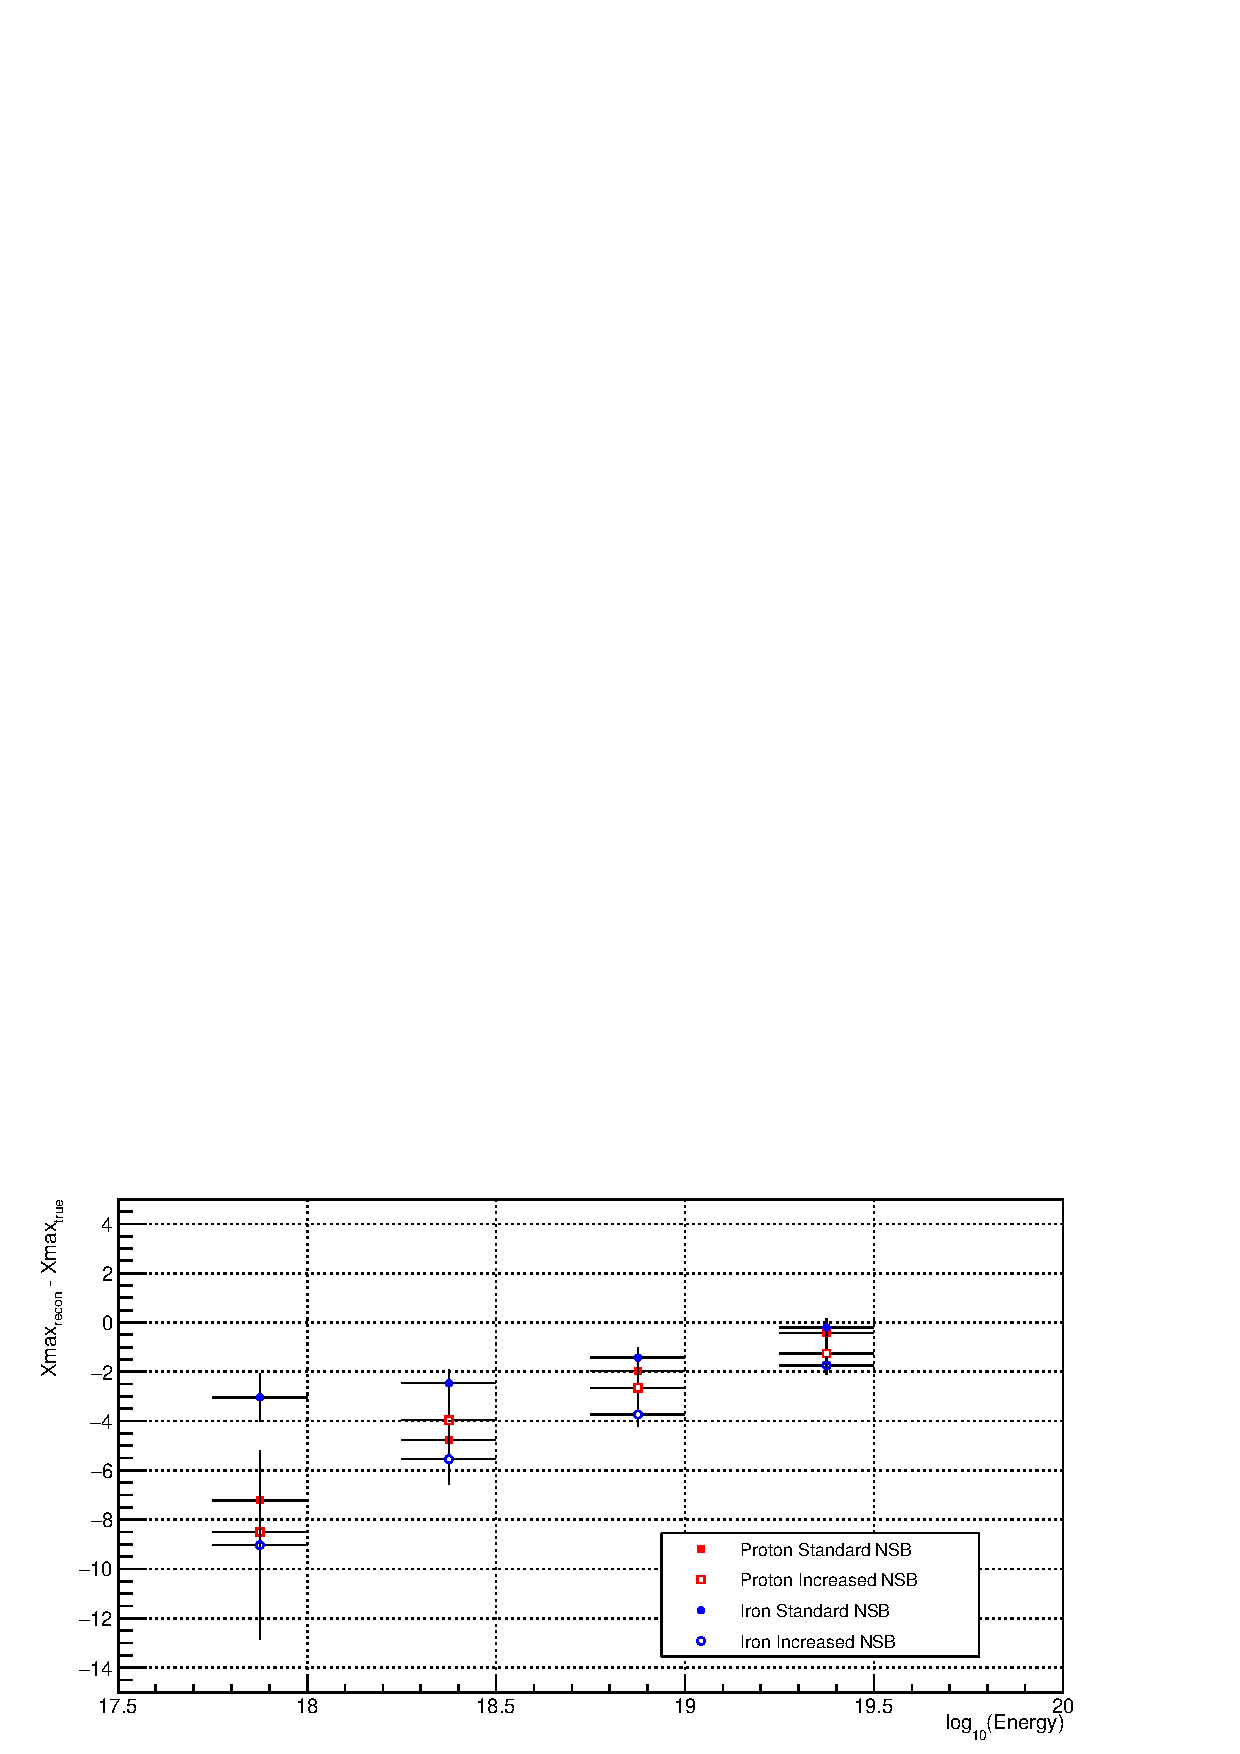
\includegraphics[width=\textwidth]{chapters/graphs/SelectionEff/Simulation_ProtonIron_XmaxBias.pdf}
\caption{Xmax Bias using simulated data.}
\end{figure}

\begin{figure}
\centering
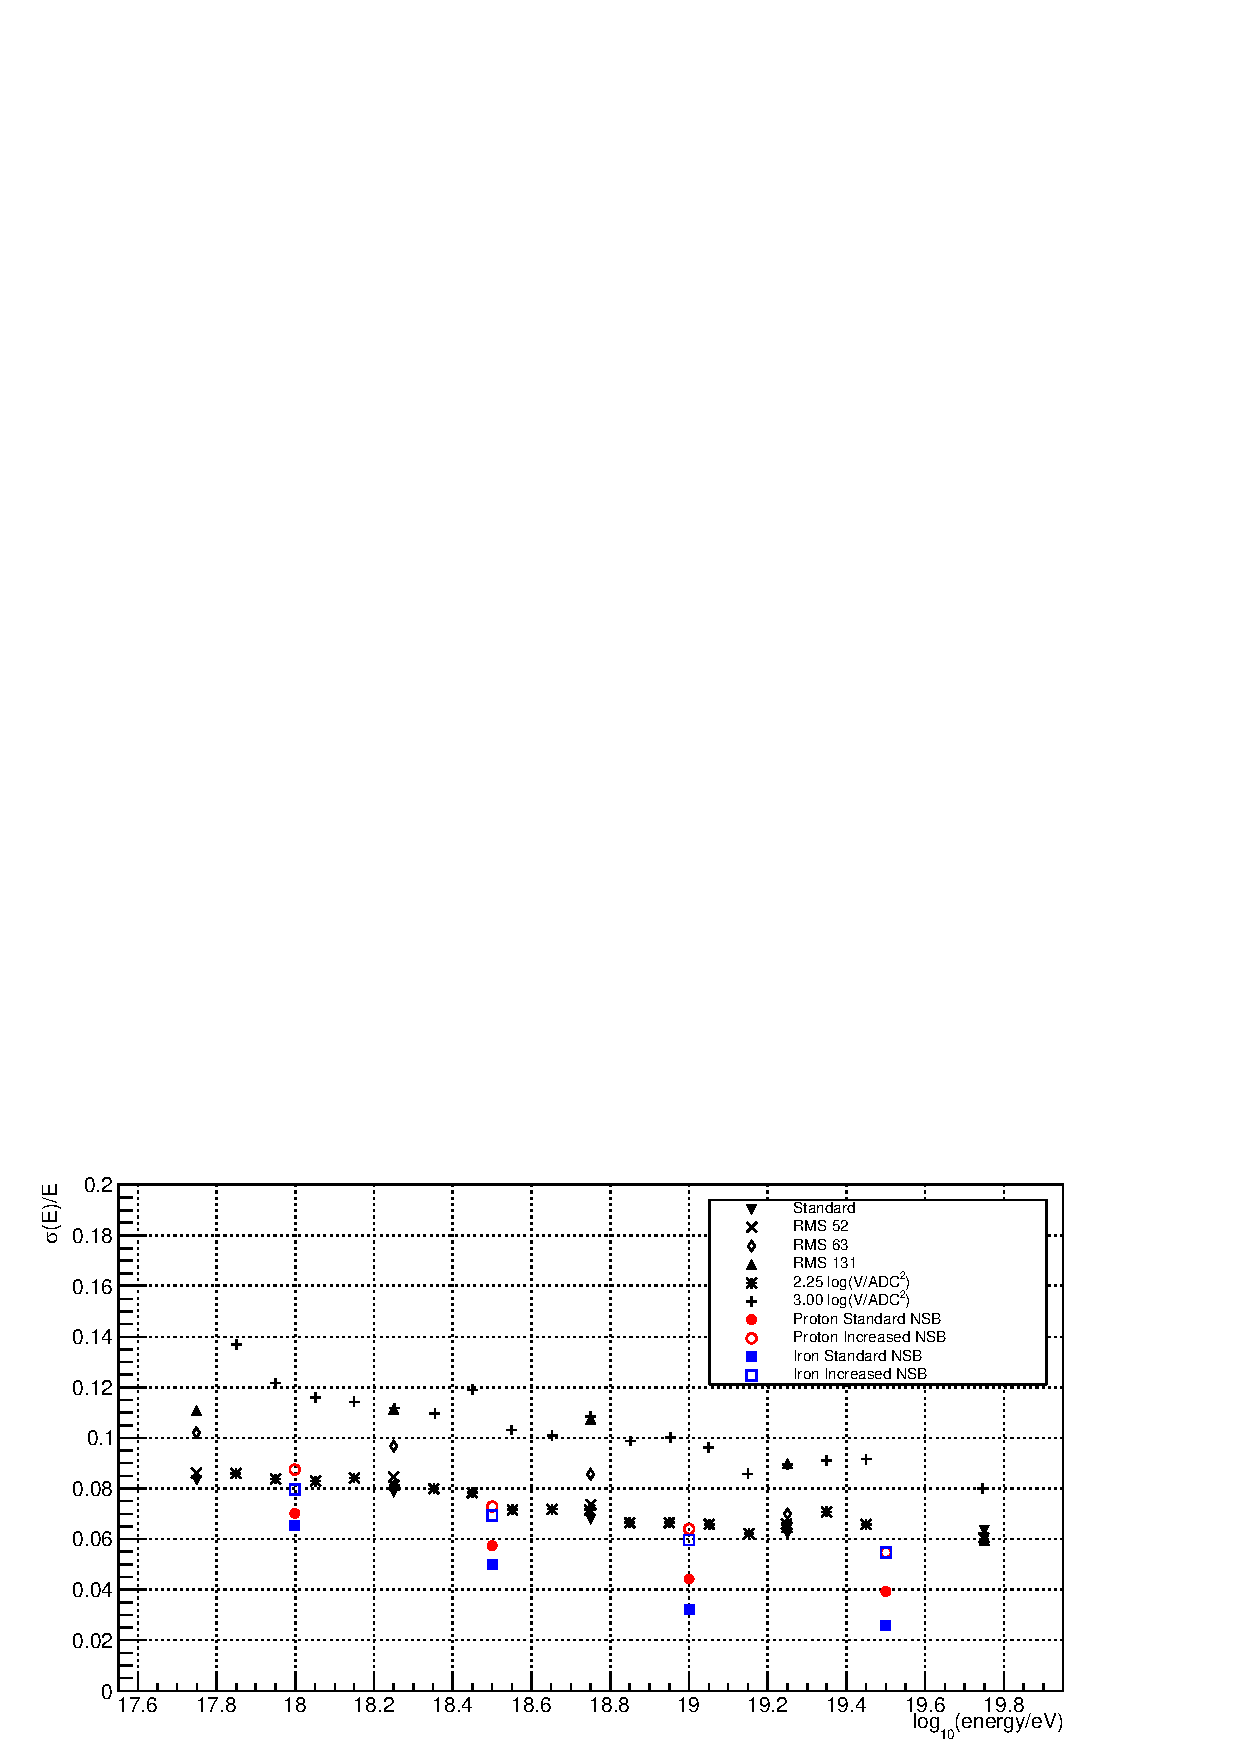
\includegraphics[width=\textwidth]{chapters/graphs/SelectionEff/Combined_EnergyRes_All.pdf}
\caption{Energy Resolution using both Smearing Method data and simulated showers.}
\vspace{3mm}
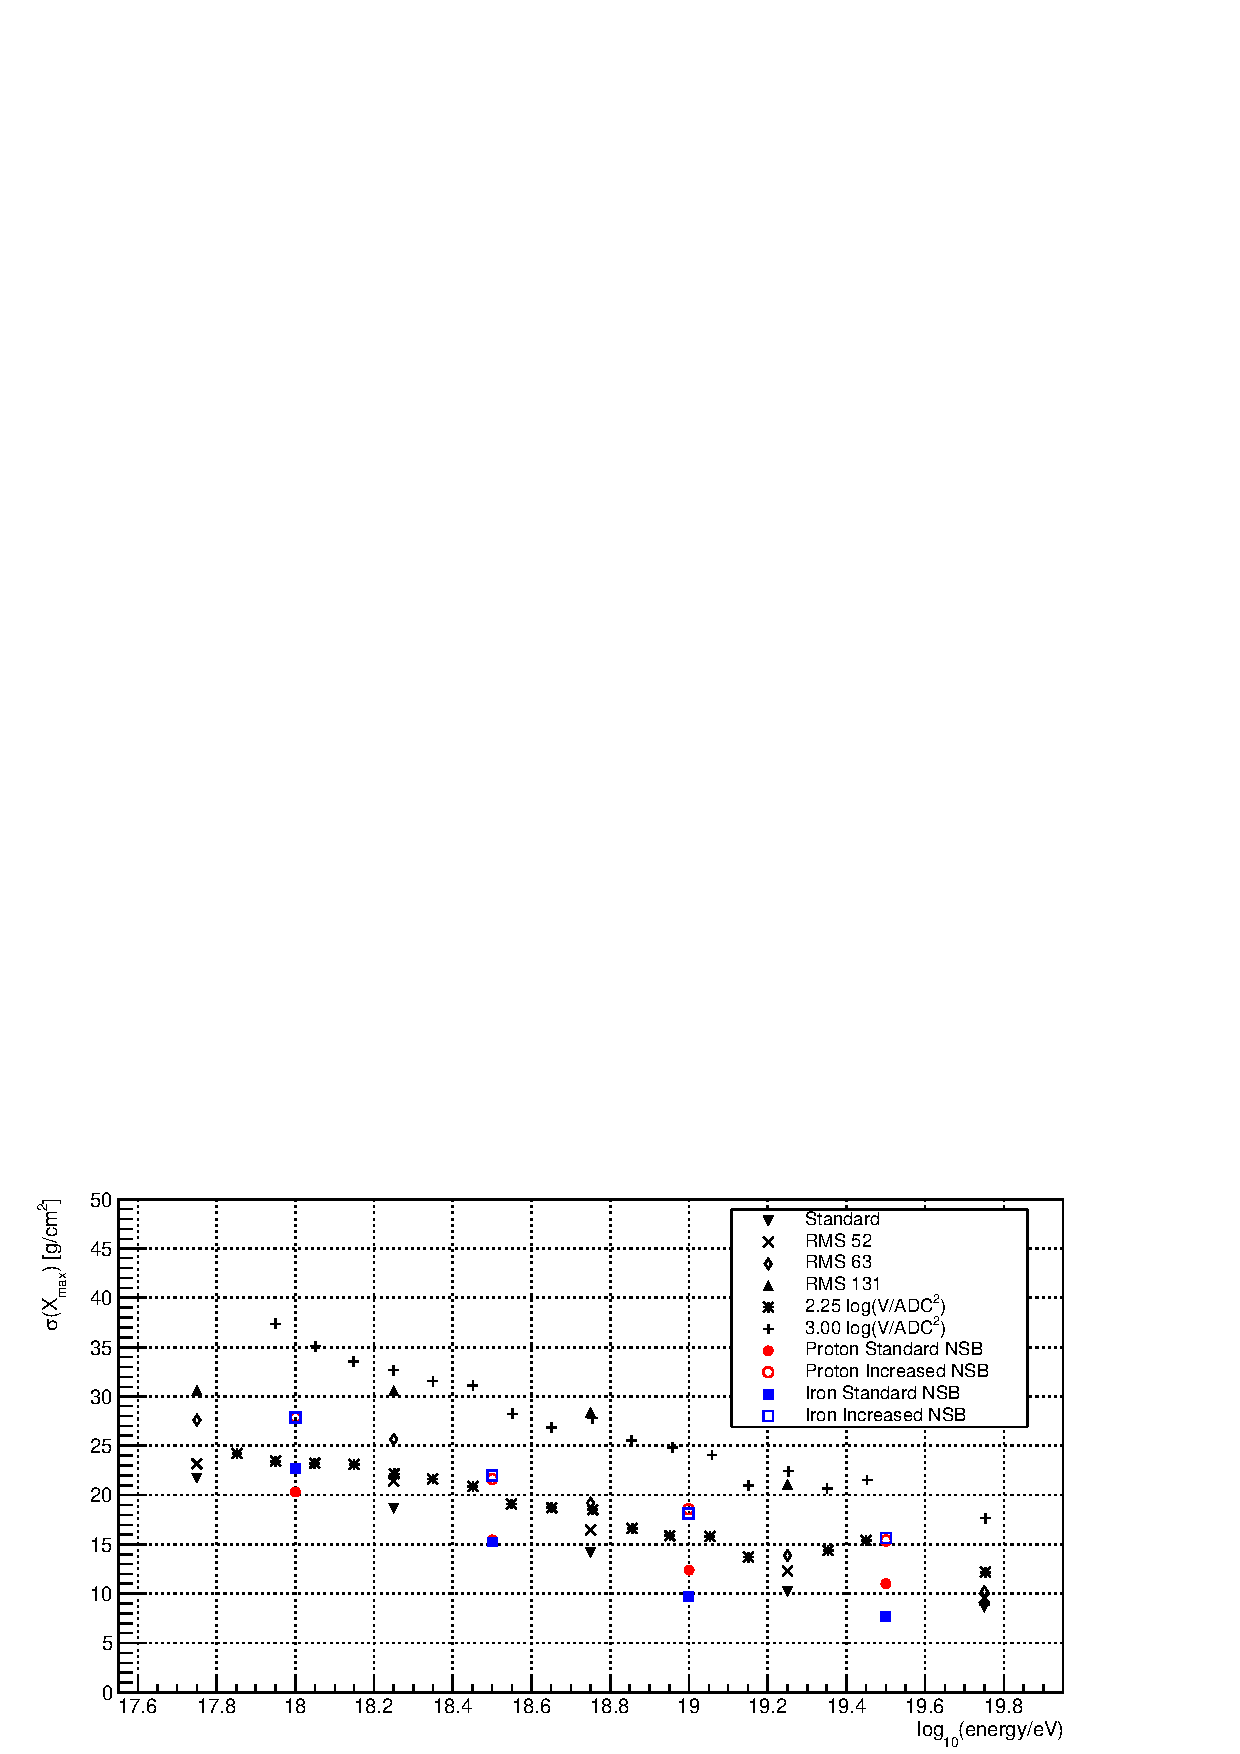
\includegraphics[width=\textwidth]{chapters/graphs/SelectionEff/Combined_XmaxRes_All.pdf}
\caption{Xmax Resolution using both Smearing Method data and simulated showers.}
\end{figure}

\begin{figure}
\centering
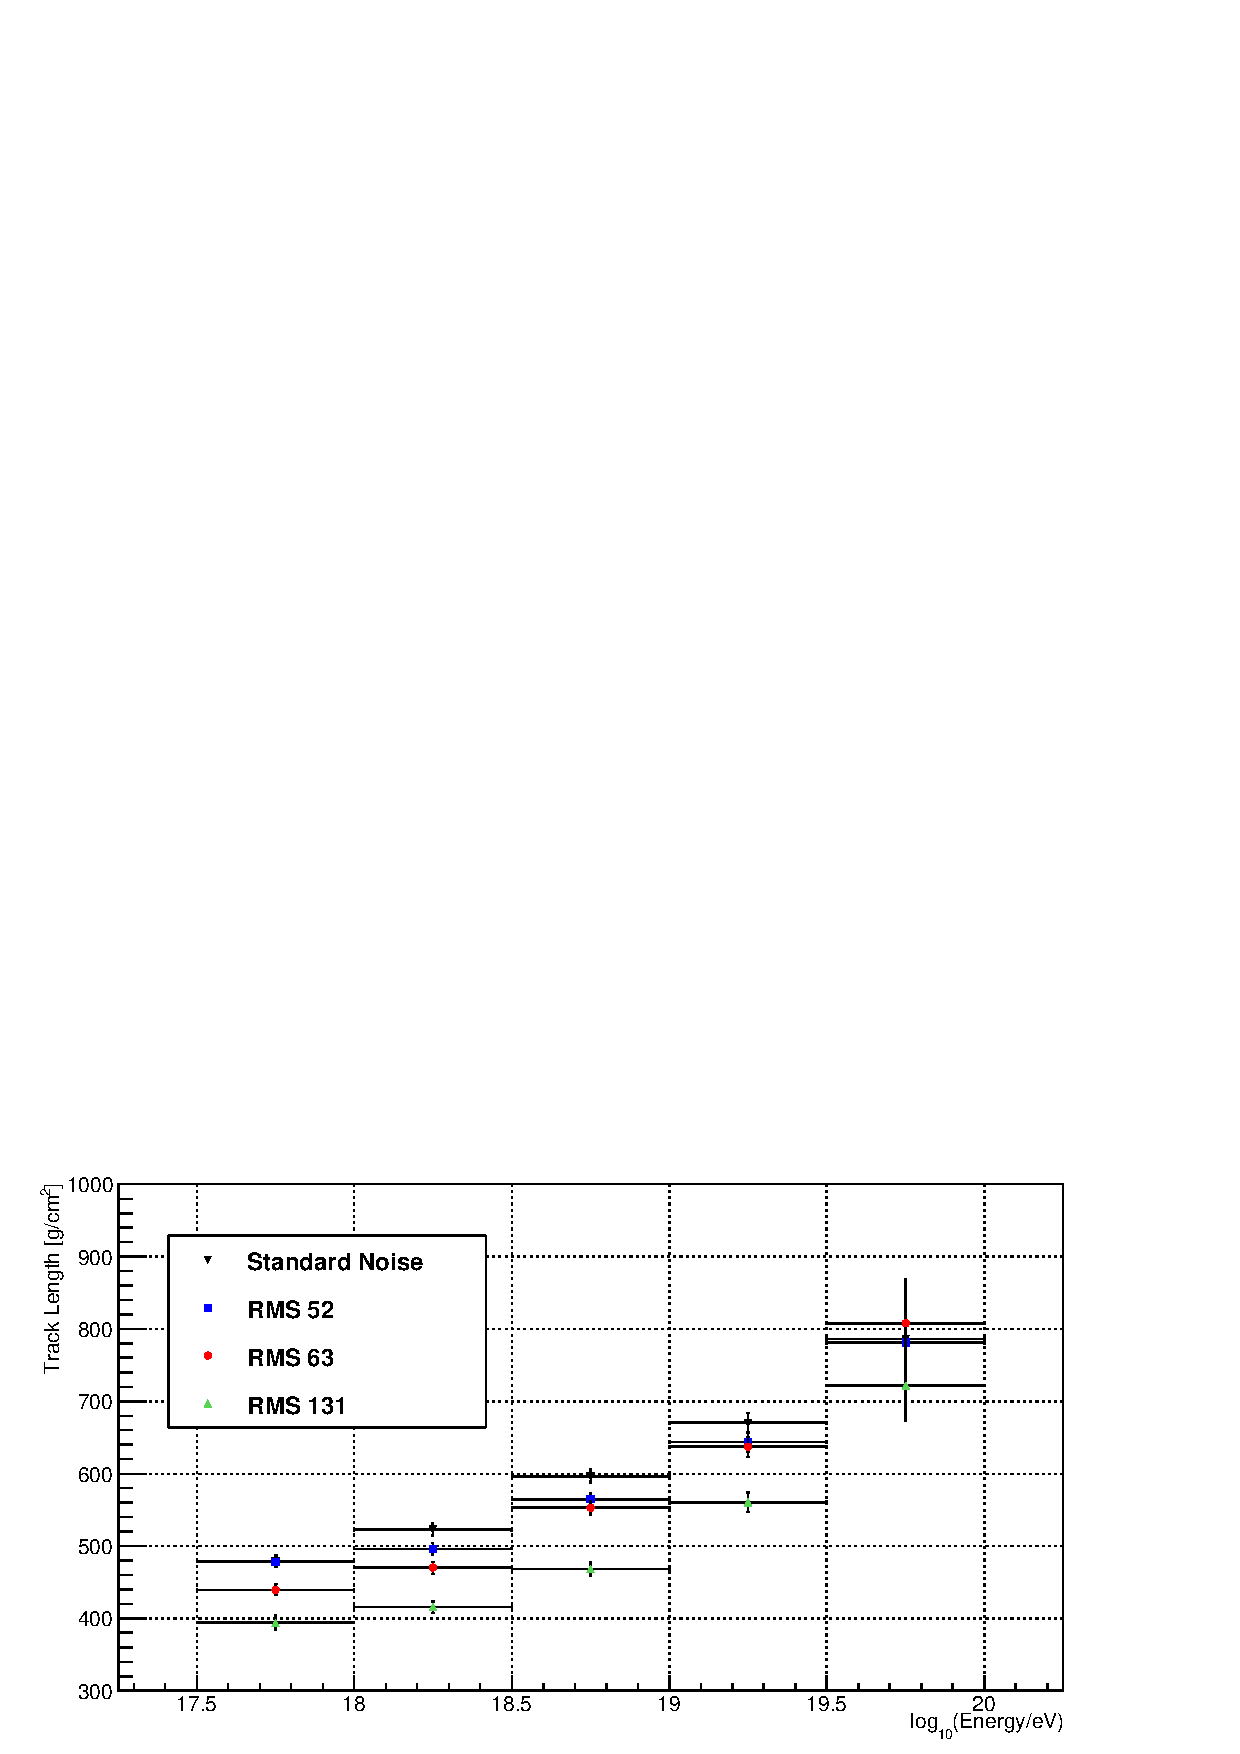
\includegraphics[width=\textwidth]{chapters/graphs/SelectionEff/Smearing_TrackLength_DiffNSBlevels.pdf}
\caption{Track length using Smearing method.} \label{fig:TrackLength_Smearing}
\end{figure}
\subsection{Discussion}

\section{Increasing NSB in Simulations to evaluate Trigger/Reconstruction Efficiency}

\subsection{Method}
 The Efficiency was calculated with the equation used:
\begin{equation}
\mathrm{Efficiency} = \mathrm{N}^{'}_{\mathrm{Select}} \ / \ \mathrm{N}^0_{\mathrm{Select}}
\end{equation}
where $\mathrm{N}^{0}_{\mathrm{Select}}$ is the number of selected events at the standard NSB level and $\mathrm{N}^{'}_{\mathrm{Select}}$ is the number of selected events at the increased NSB
level. 

After the Efficiency was calculated the bias and resolution for Xmax and energy was determined. For real data, the bias is the relative change in the mean of the distributions at increased NSB to the mean of the distributions at standard NSB, both after reconstruction and selection cuts. The bias calculations for real data become:
\begin{eqnarray}
\Delta \mathrm{E}_{\mathrm{Data}} &=& \frac{\mathrm{E}_{\mathrm{IncreasedNSB}} - \mathrm{E}_{\mathrm{StandardNSB}}}{\mathrm{E}_{\mathrm{StandardNSB}}} \label{eq:energybias_data} \\
\Delta \mathrm{Xmax}_{\mathrm{Data}} &=& \mathrm{Xmax}_{\mathrm{IncreasedNSB}} - \mathrm{Xmax}_{\mathrm{StandardNSB}}\label{eq:xmaxbias_data}
\end{eqnarray} 
For simulated data the bias is the relative change in the mean of the distributions after the full simulation by EAS events going through an atmosphere with a specified NSB photon field, the FD telescopes optics, trigger, reconstruction and selection cuts compared with Monte-Carlo truth.
\begin{eqnarray}
\Delta \mathrm{E}_{\mathrm{Sim}} &=& \frac{\mathrm{E}_{\mathrm{recon}} - \mathrm{E}_{\mathrm{true}}}{\mathrm{E}_{\mathrm{true}}}  \label{eq:energybias_sim} \\
\Delta \mathrm{Xmax}_{\mathrm{Sim}} &=& \mathrm{Xmax}_{\mathrm{recon}} - \mathrm{Xmax}_{\mathrm{true}} \label{eq:xmaxbias_sim}
\end{eqnarray}
 
 
The energy and Xmax resolution is calculated via:
\begin{eqnarray}
\sigma_{\mathrm{res}} &=& \left( \frac{1}{\mathrm{N}} \sum \frac{1}{\sigma^2_i} \right)^{1/2}
\end{eqnarray}

\subsection{Comparison of Simulated Data to Real Data}
\begin{figure}
\centering
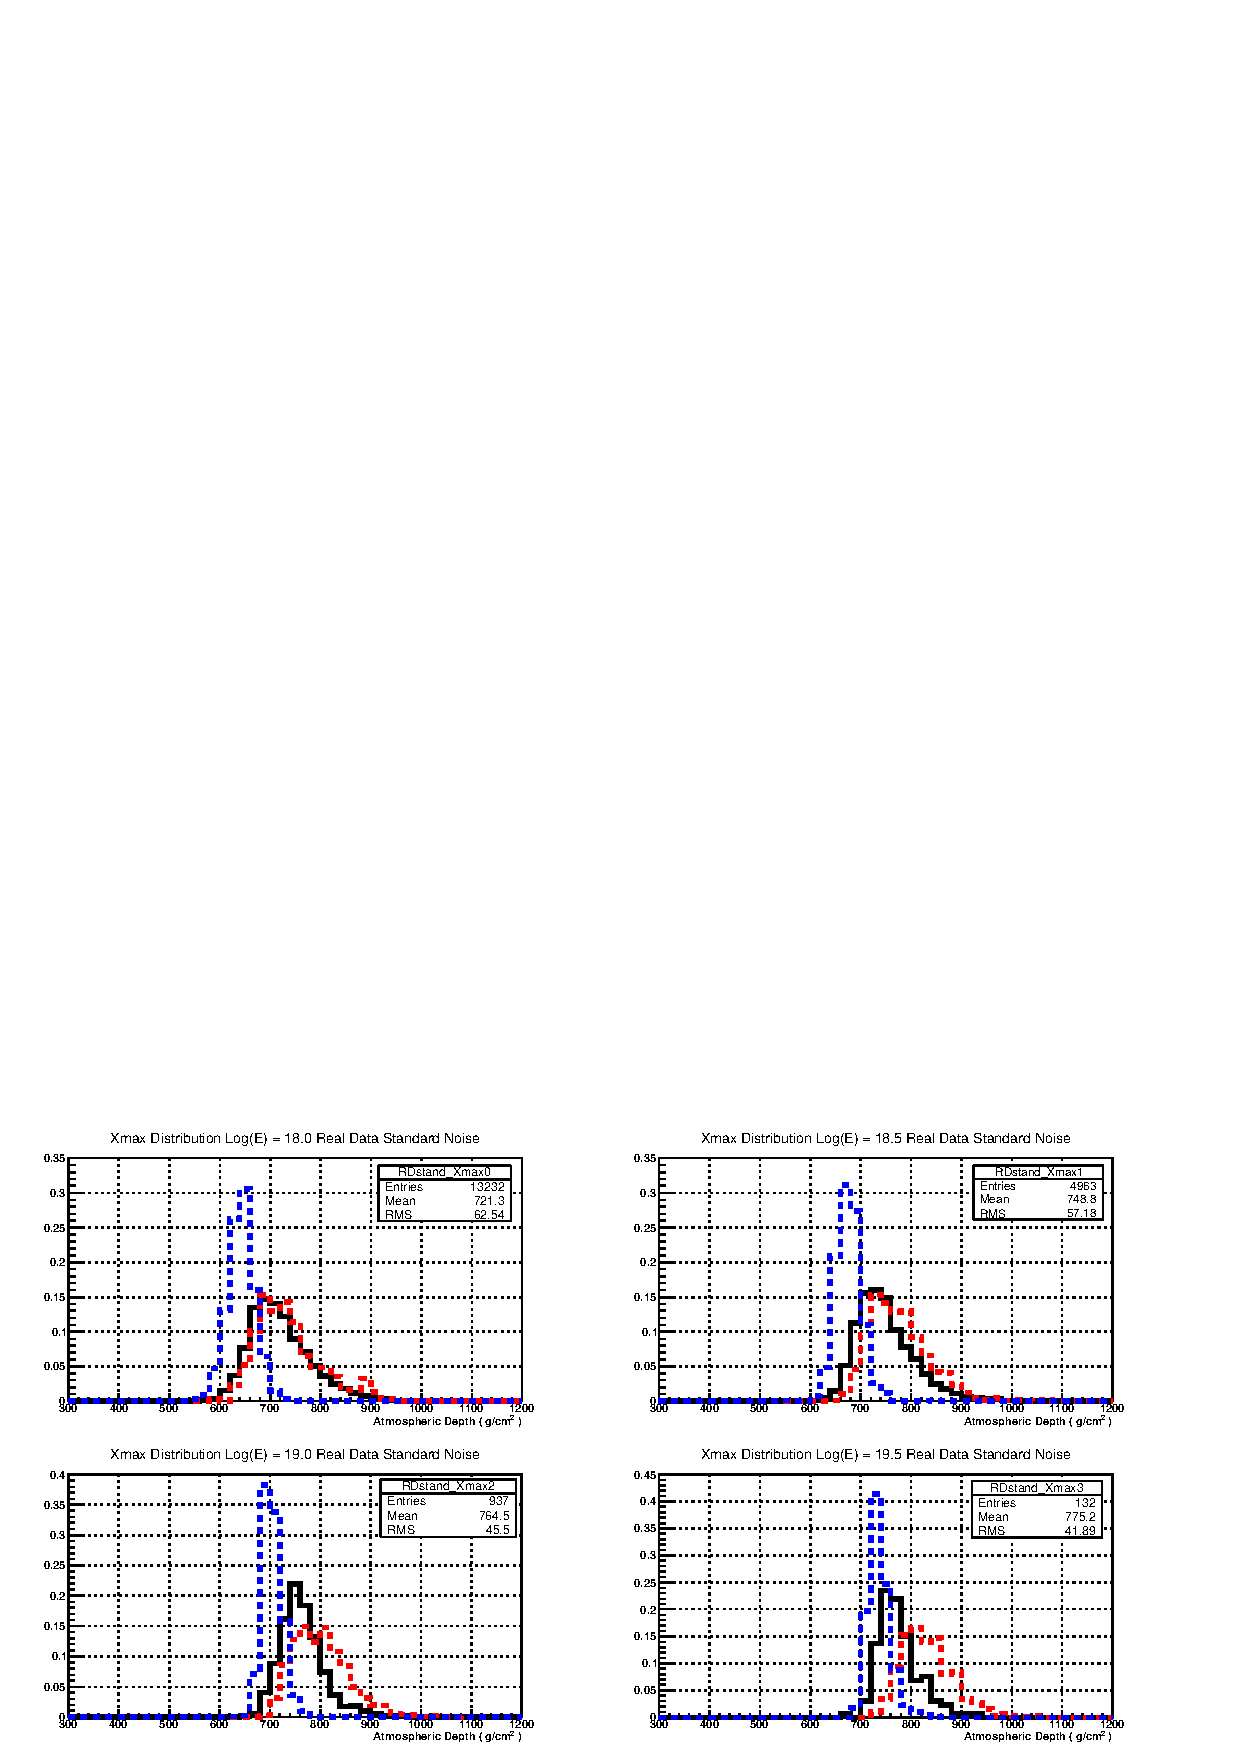
\includegraphics[width=\textwidth]{chapters/graphs/SelectionEff/RealDataAndSim_XmaxDistComp.pdf}
\caption{Distribution of Xmax with Real Data and simulation of proton and iron showers.}
\vspace{3mm}
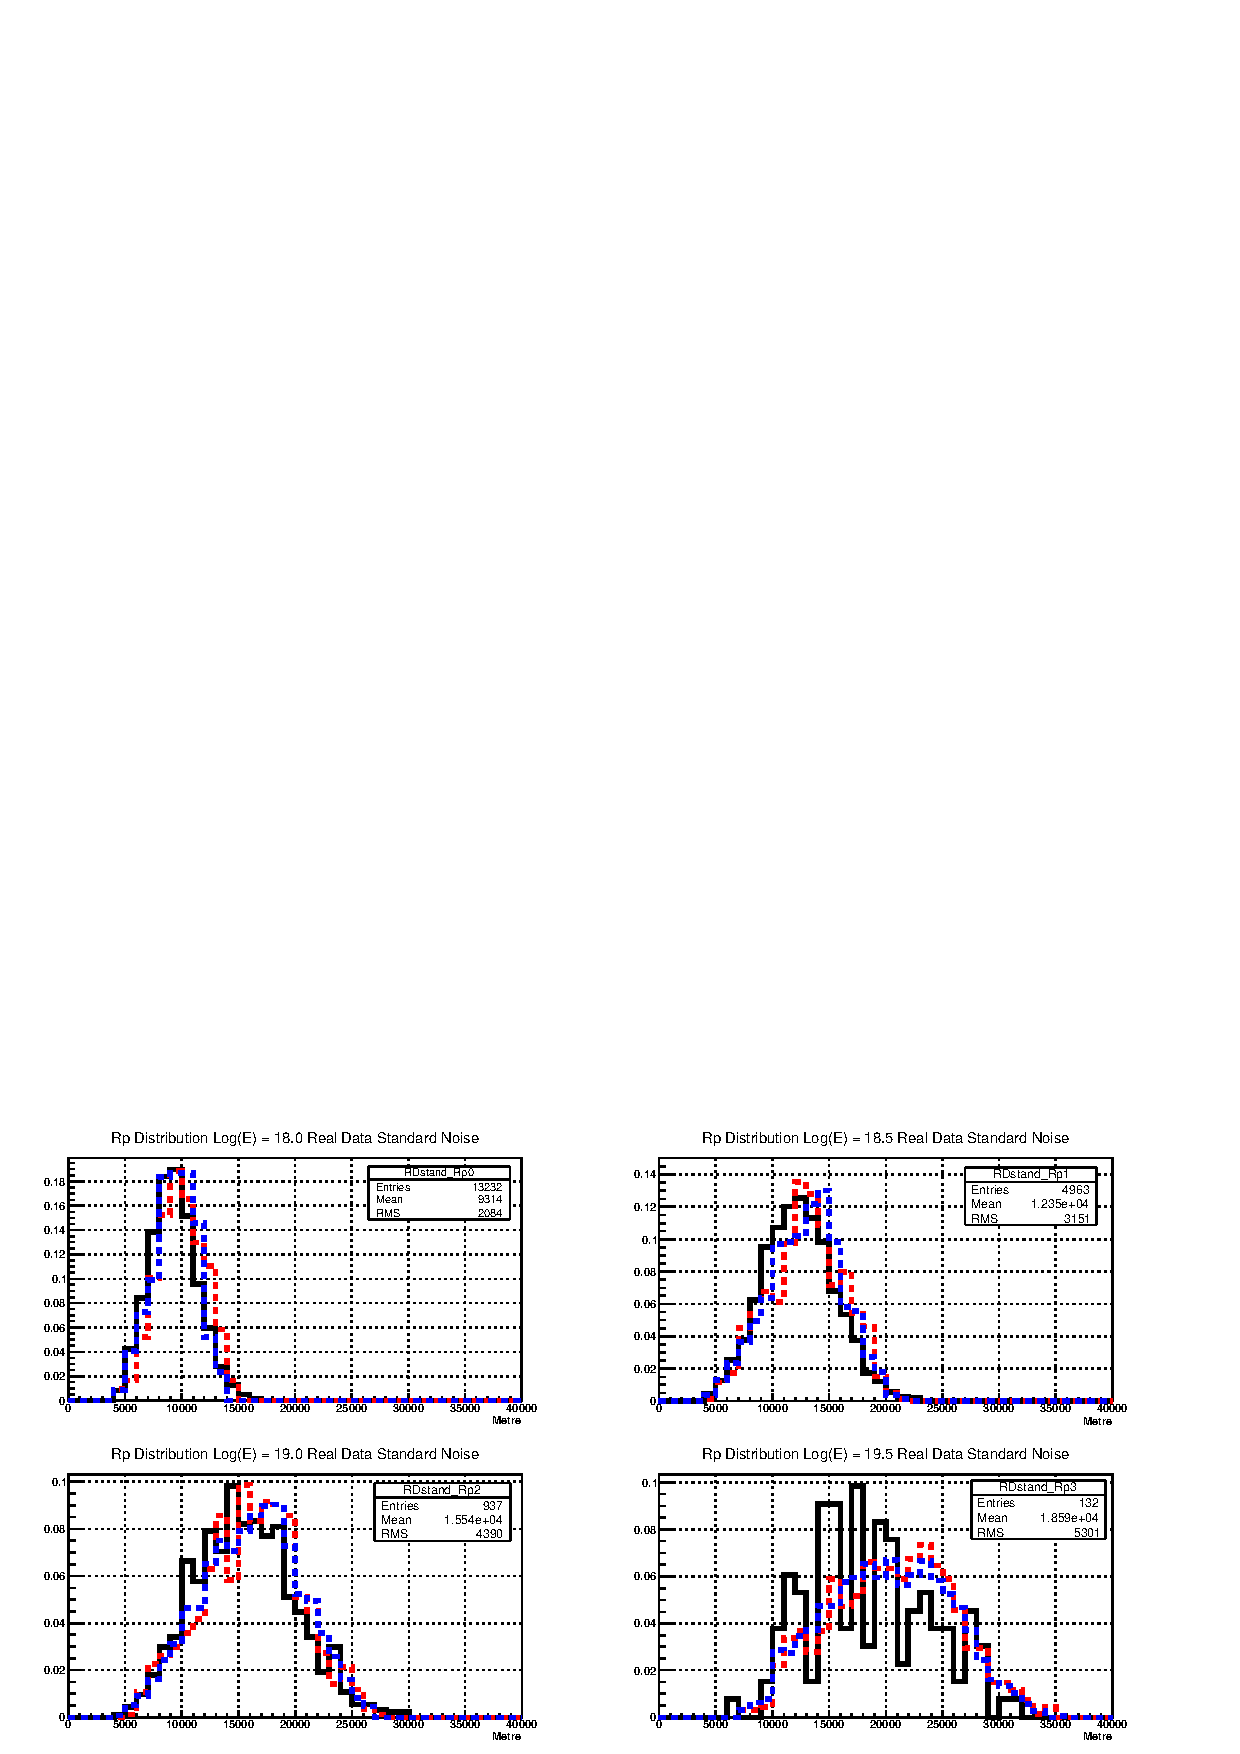
\includegraphics[width=\textwidth]{chapters/graphs/SelectionEff/RealDataAndSim_RpDistComp.pdf}
\caption{Distribution of Rp with Real Data and simulation of proton and iron showers.}
\end{figure}

\begin{figure}
\centering
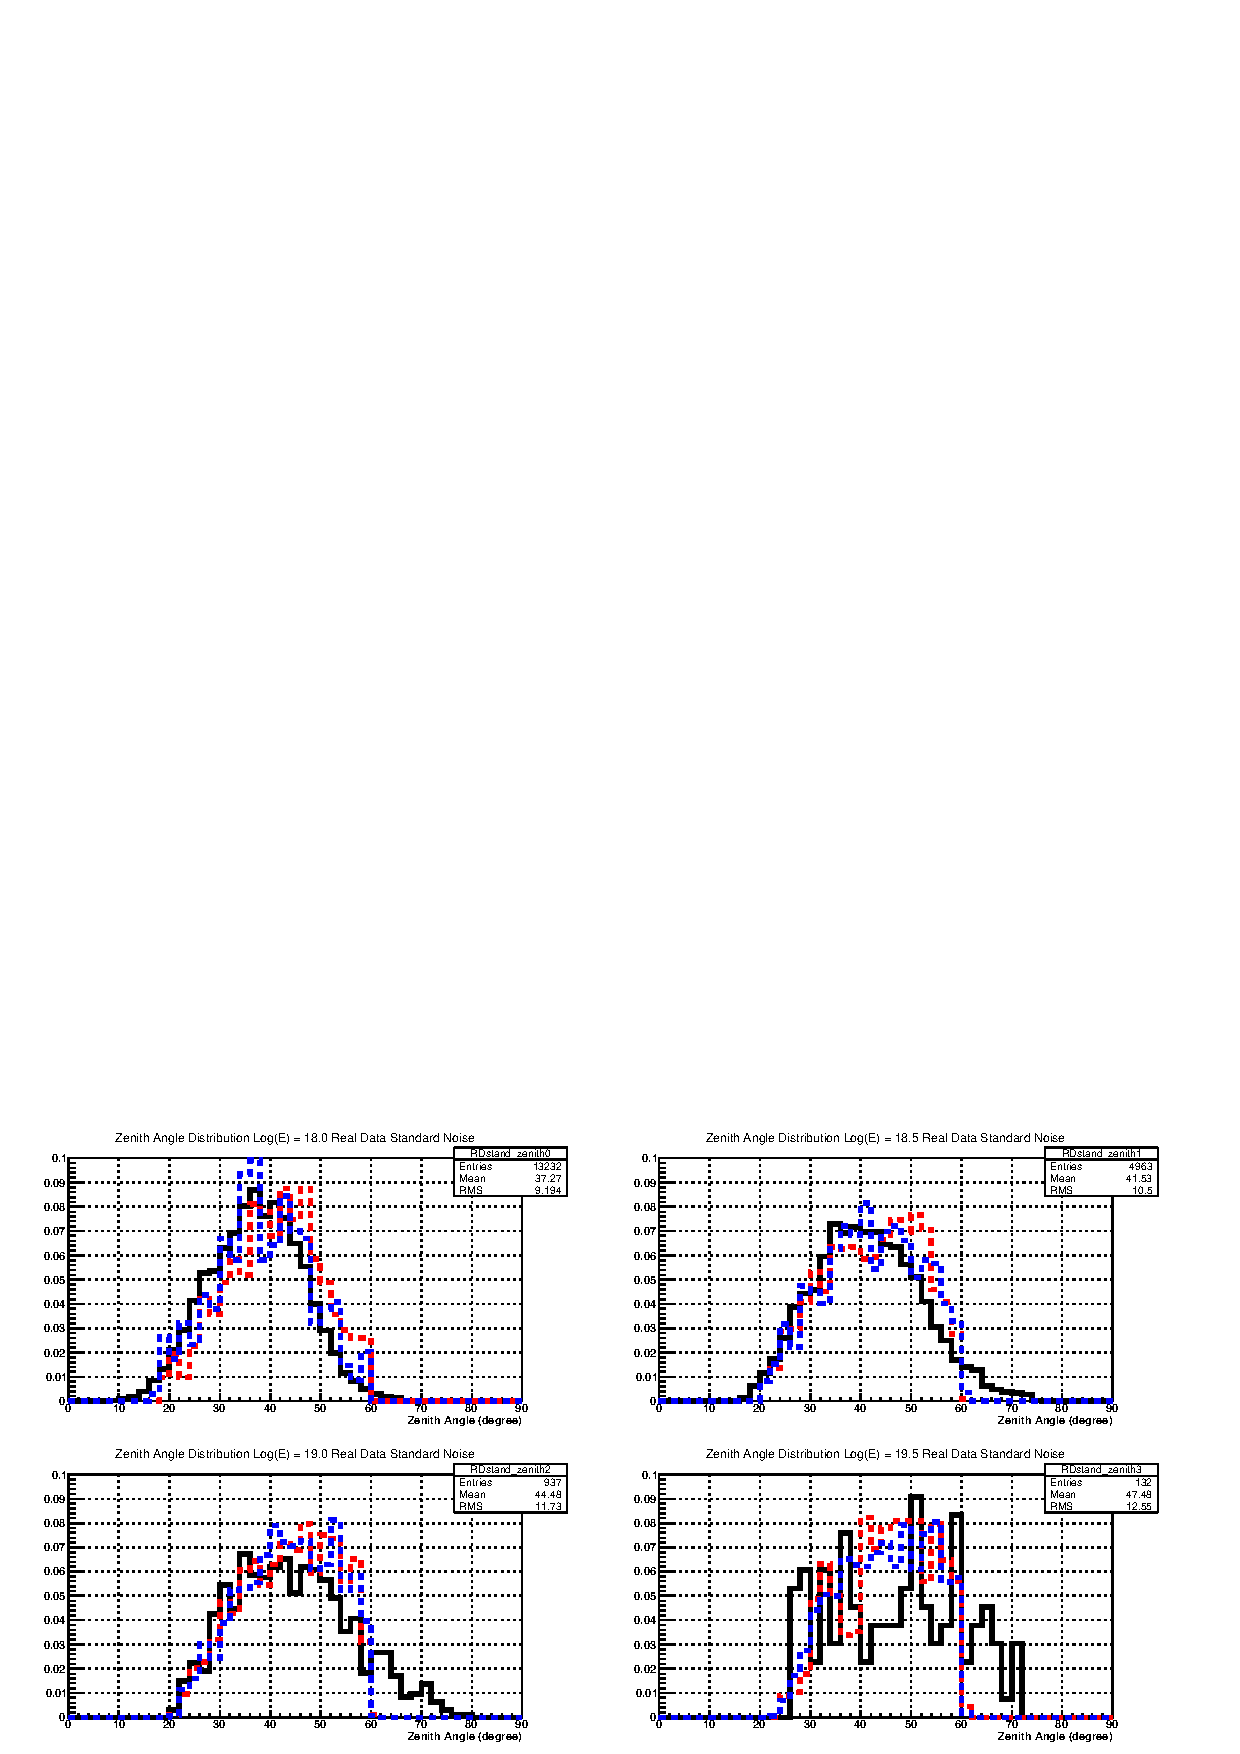
\includegraphics[width=\textwidth]{chapters/graphs/SelectionEff/RealDataAndSim_ZenithDistComp.pdf}
\caption{Distribution of Zenith angle with Real Data and simulation of proton and iron showers.}
\vspace{3mm}
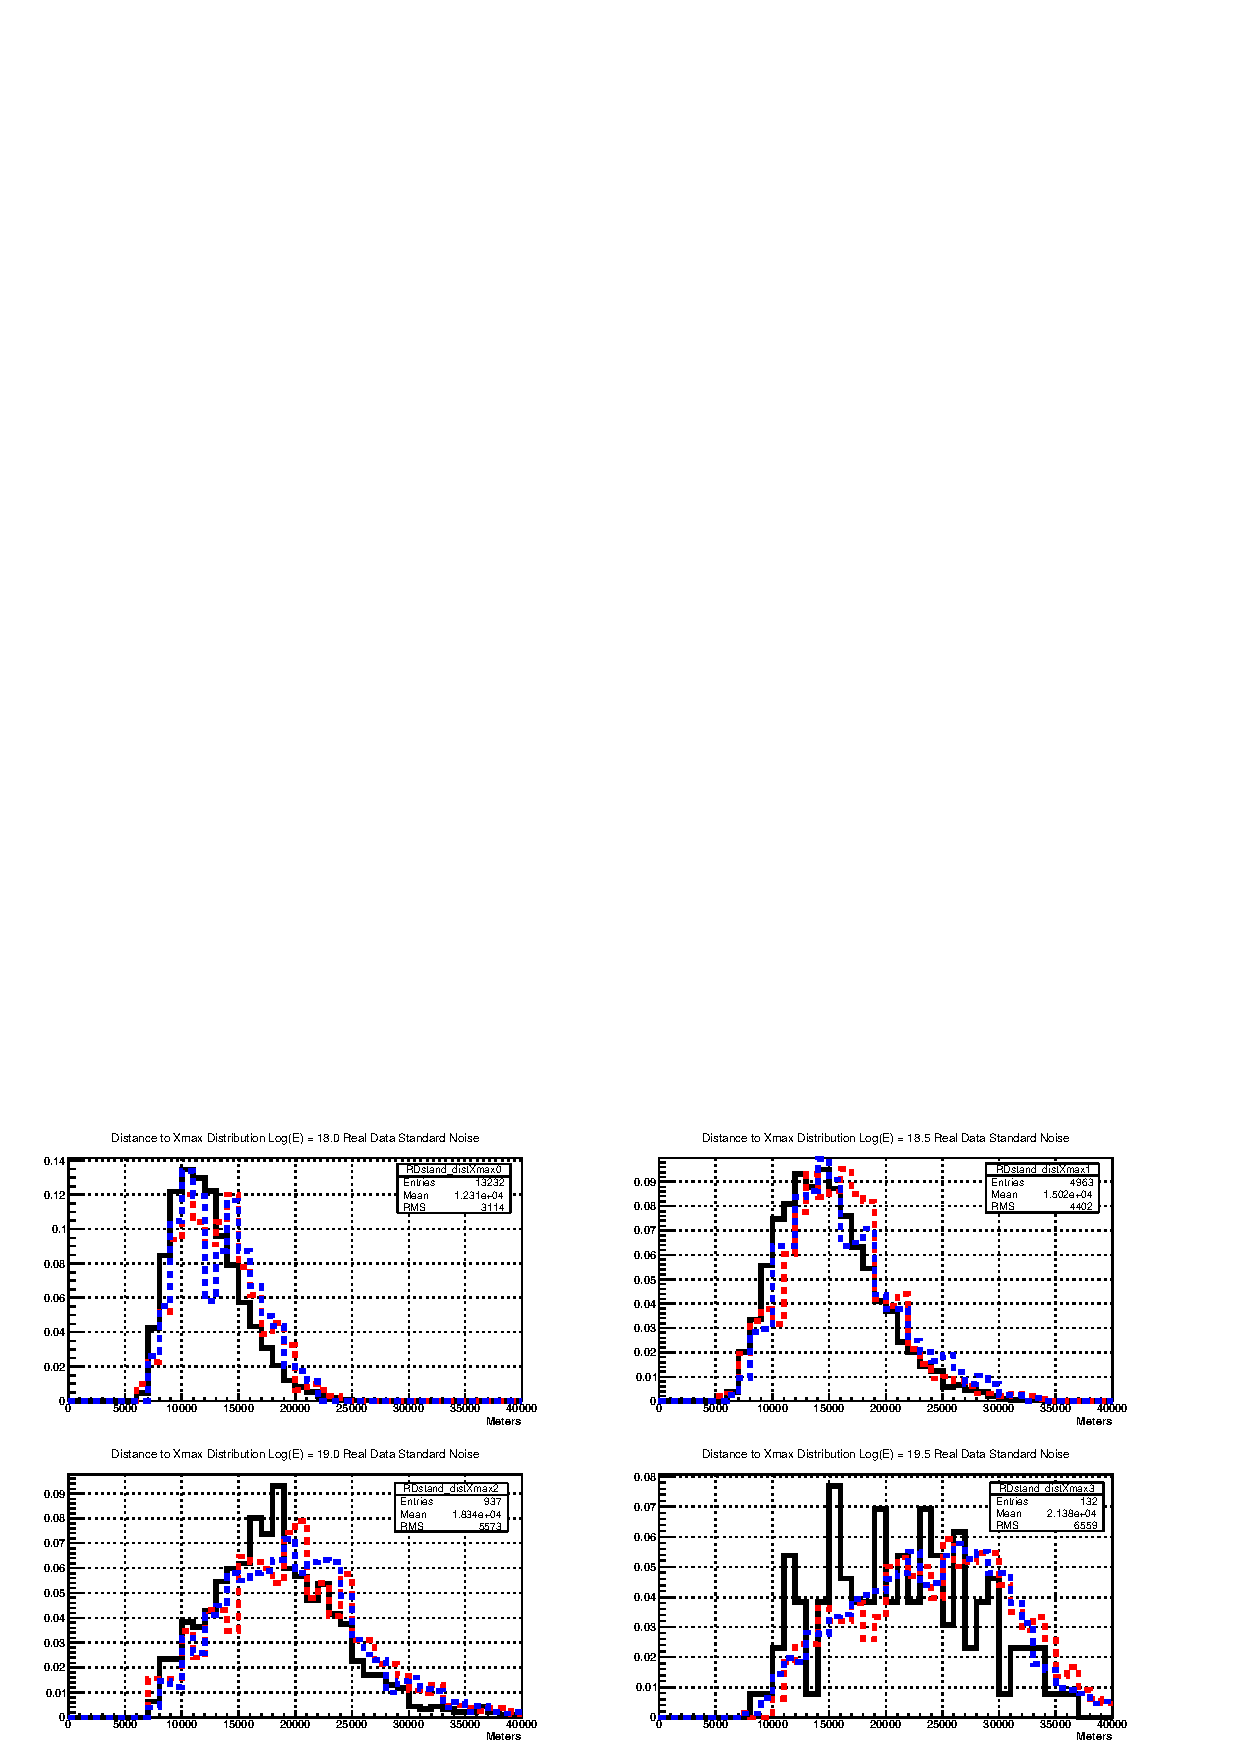
\includegraphics[width=\textwidth]{chapters/graphs/SelectionEff/RealDataAndSim_DistToXmaxDistComp.pdf}
\caption{Distribution of Distance to Xmax with Real Data and simulation of proton and iron showers.}
\end{figure}

\subsection{Results}
\begin{figure}
\centering
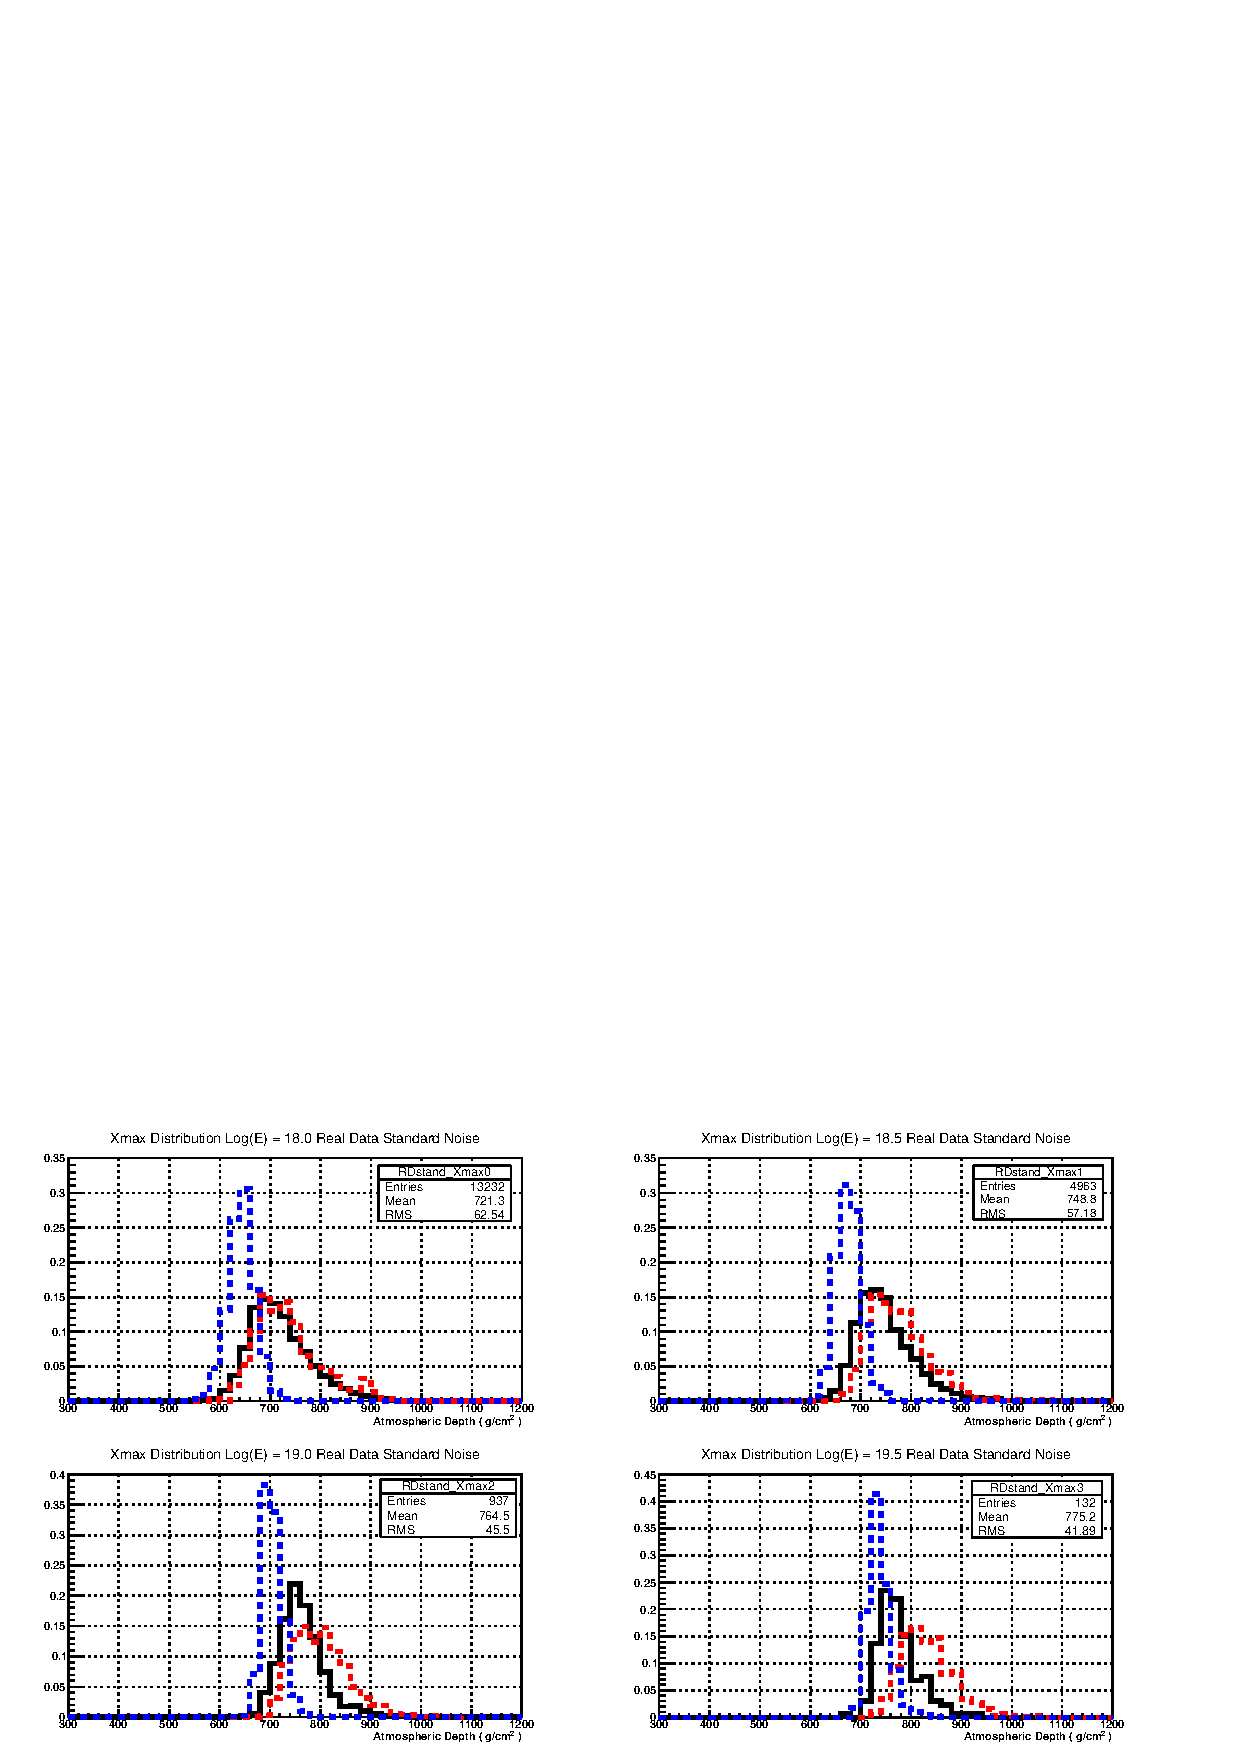
\includegraphics[width=\textwidth]{chapters/graphs/SelectionEff/RealDataAndSim_XmaxDistComp.pdf}
\caption{Distribution of Xmax with Real Data and simulation of proton and iron showers.}
\vspace{3mm}
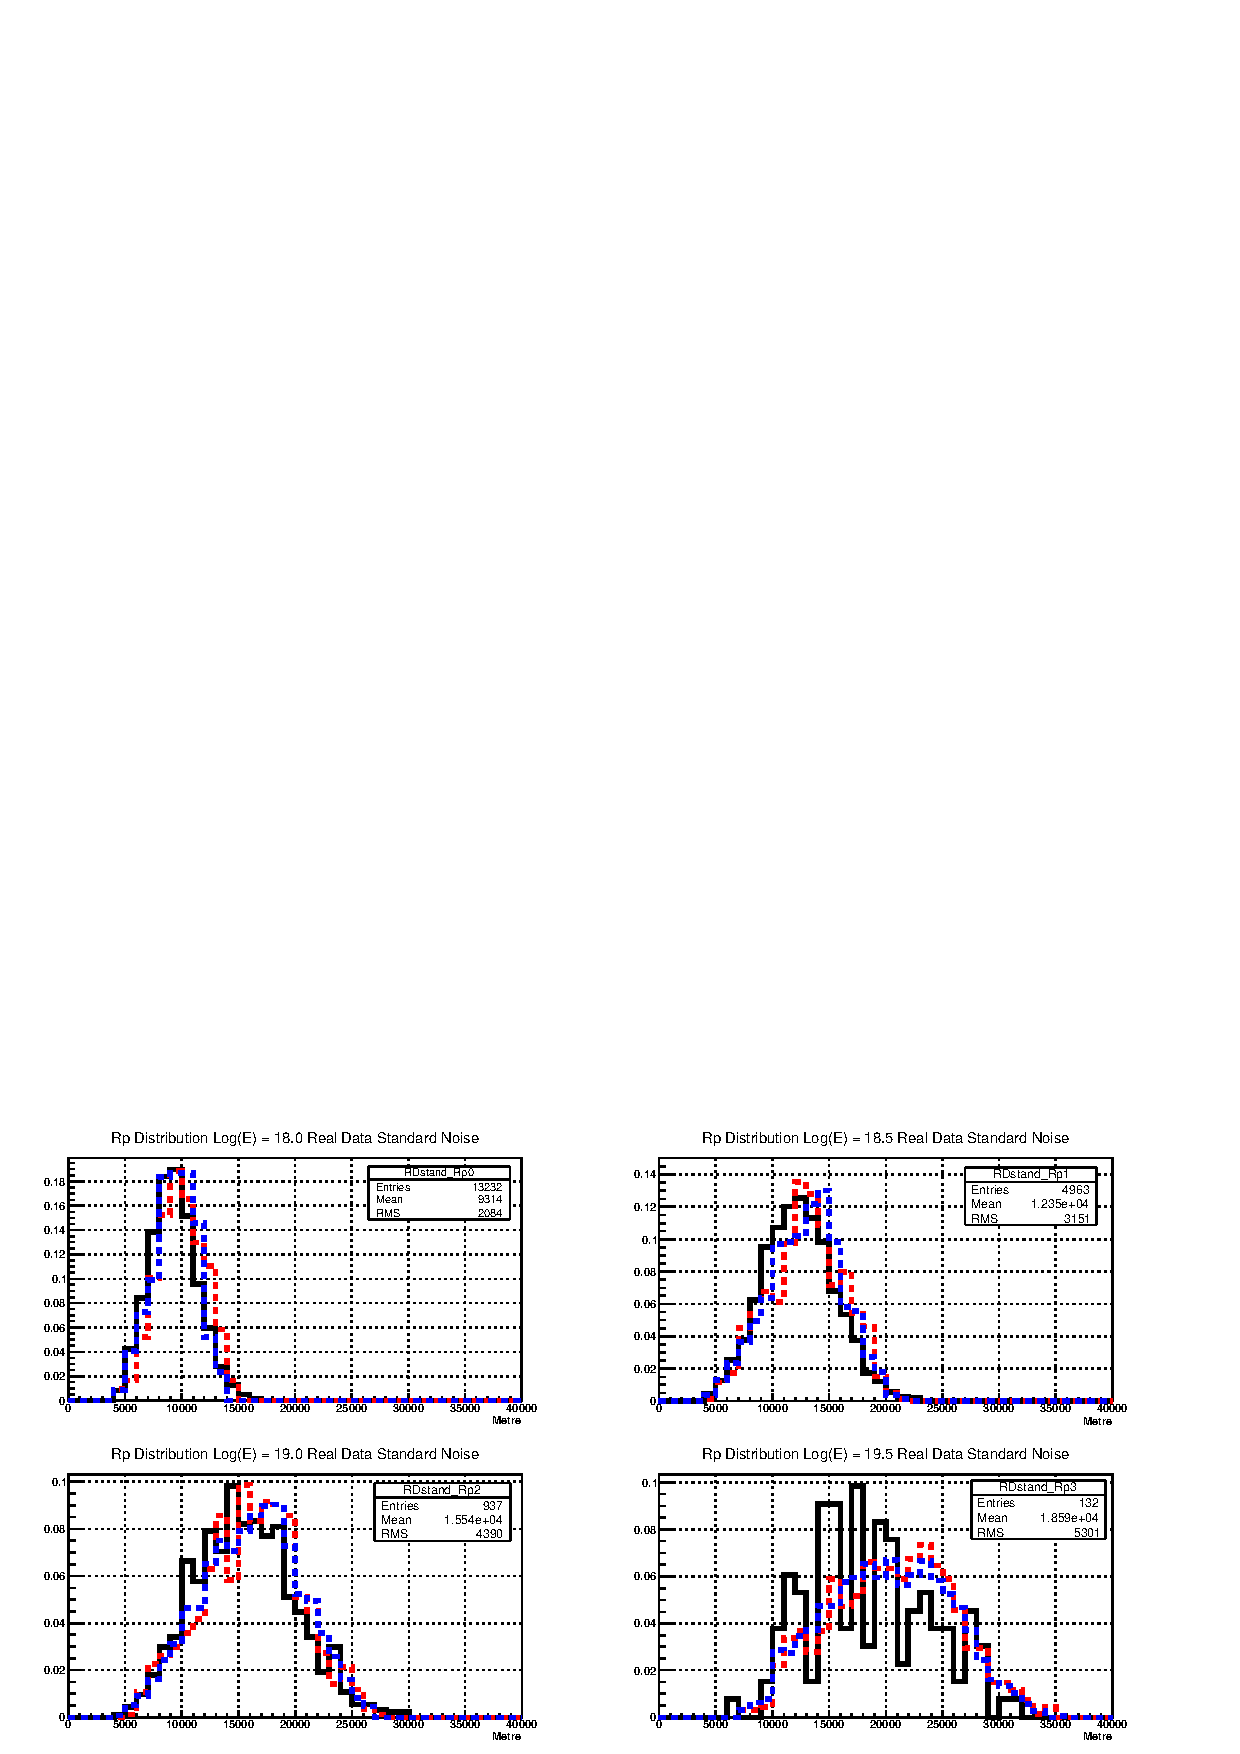
\includegraphics[width=\textwidth]{chapters/graphs/SelectionEff/RealDataAndSim_RpDistComp.pdf}
\caption{Distribution of Rp with Real Data and simulation of proton and iron showers.}
\end{figure}

\begin{figure}
\centering
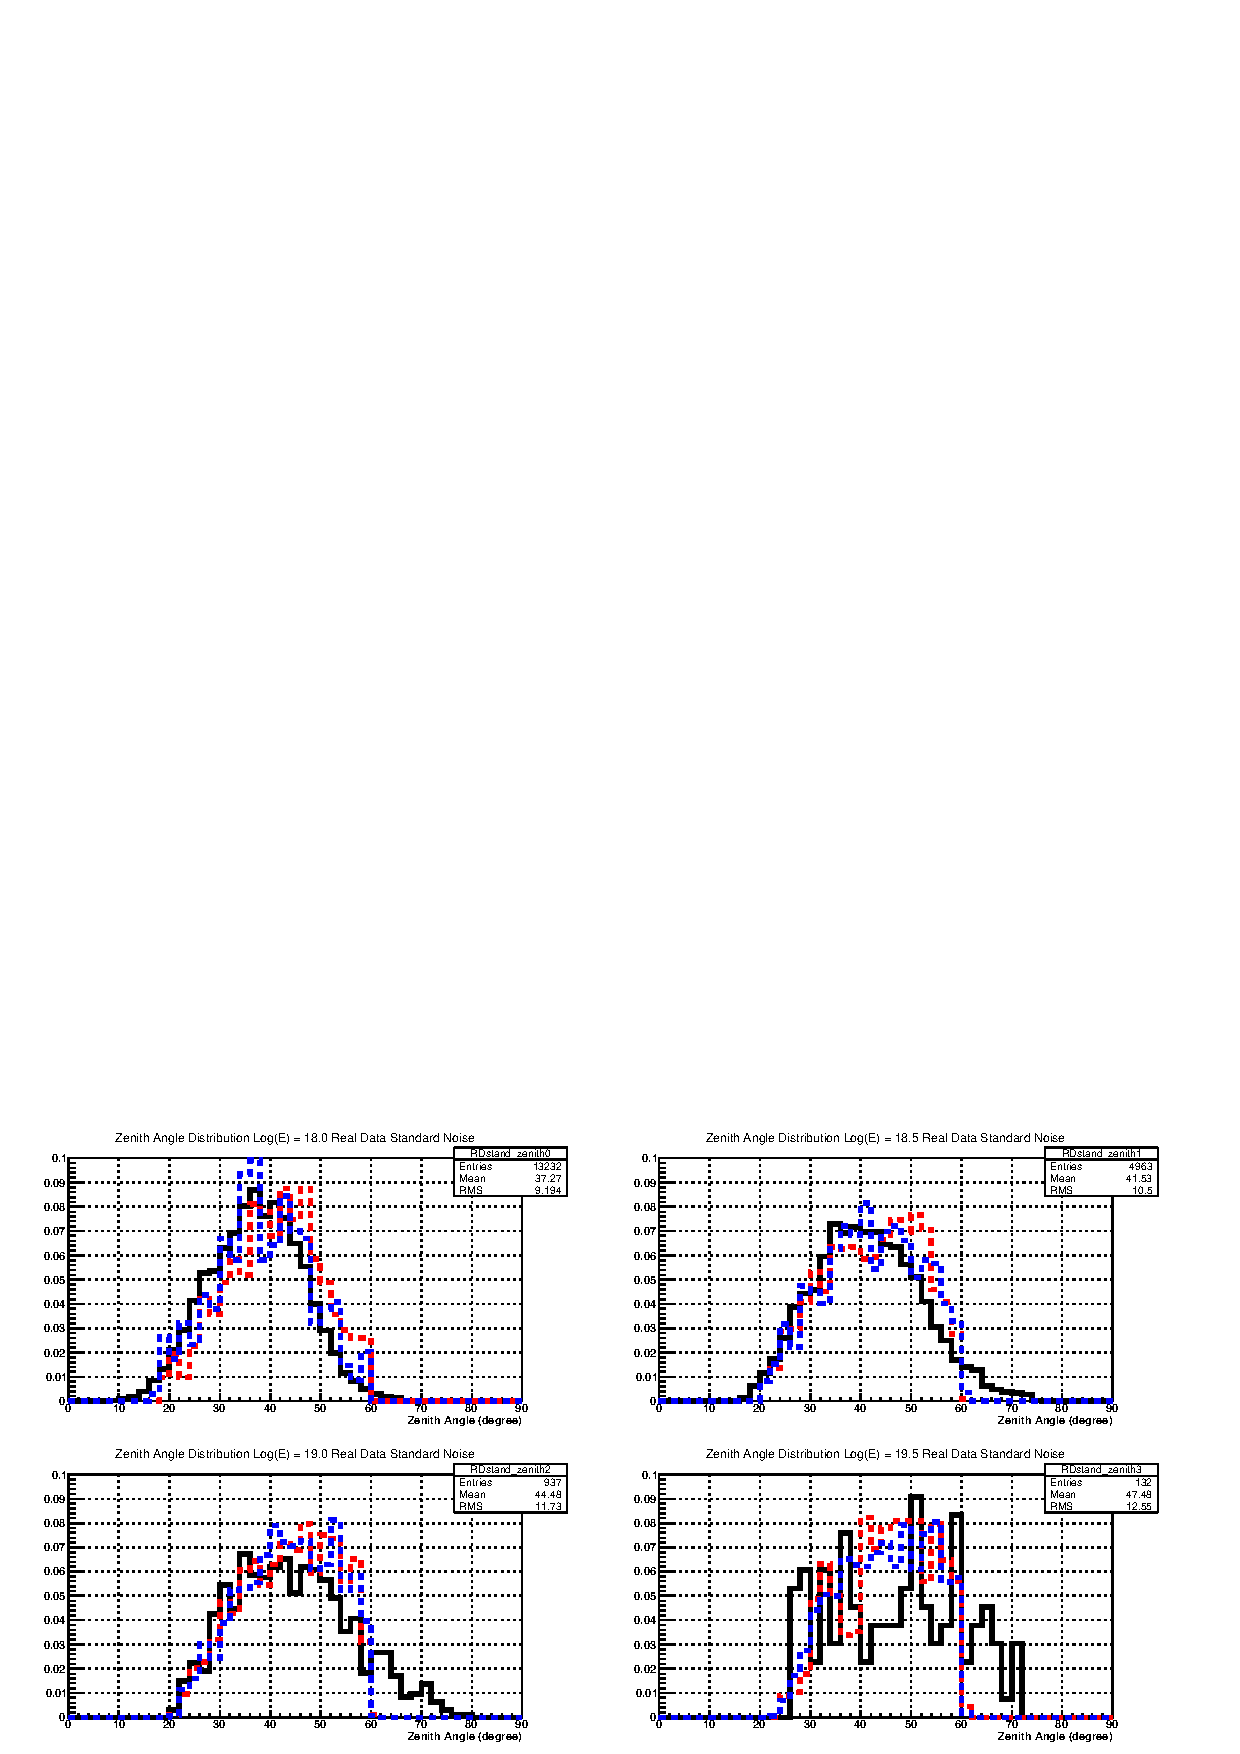
\includegraphics[width=\textwidth]{chapters/graphs/SelectionEff/RealDataAndSim_ZenithDistComp.pdf}
\caption{Distribution of Zenith angle with Real Data and simulation of proton and iron showers.}
\vspace{3mm}
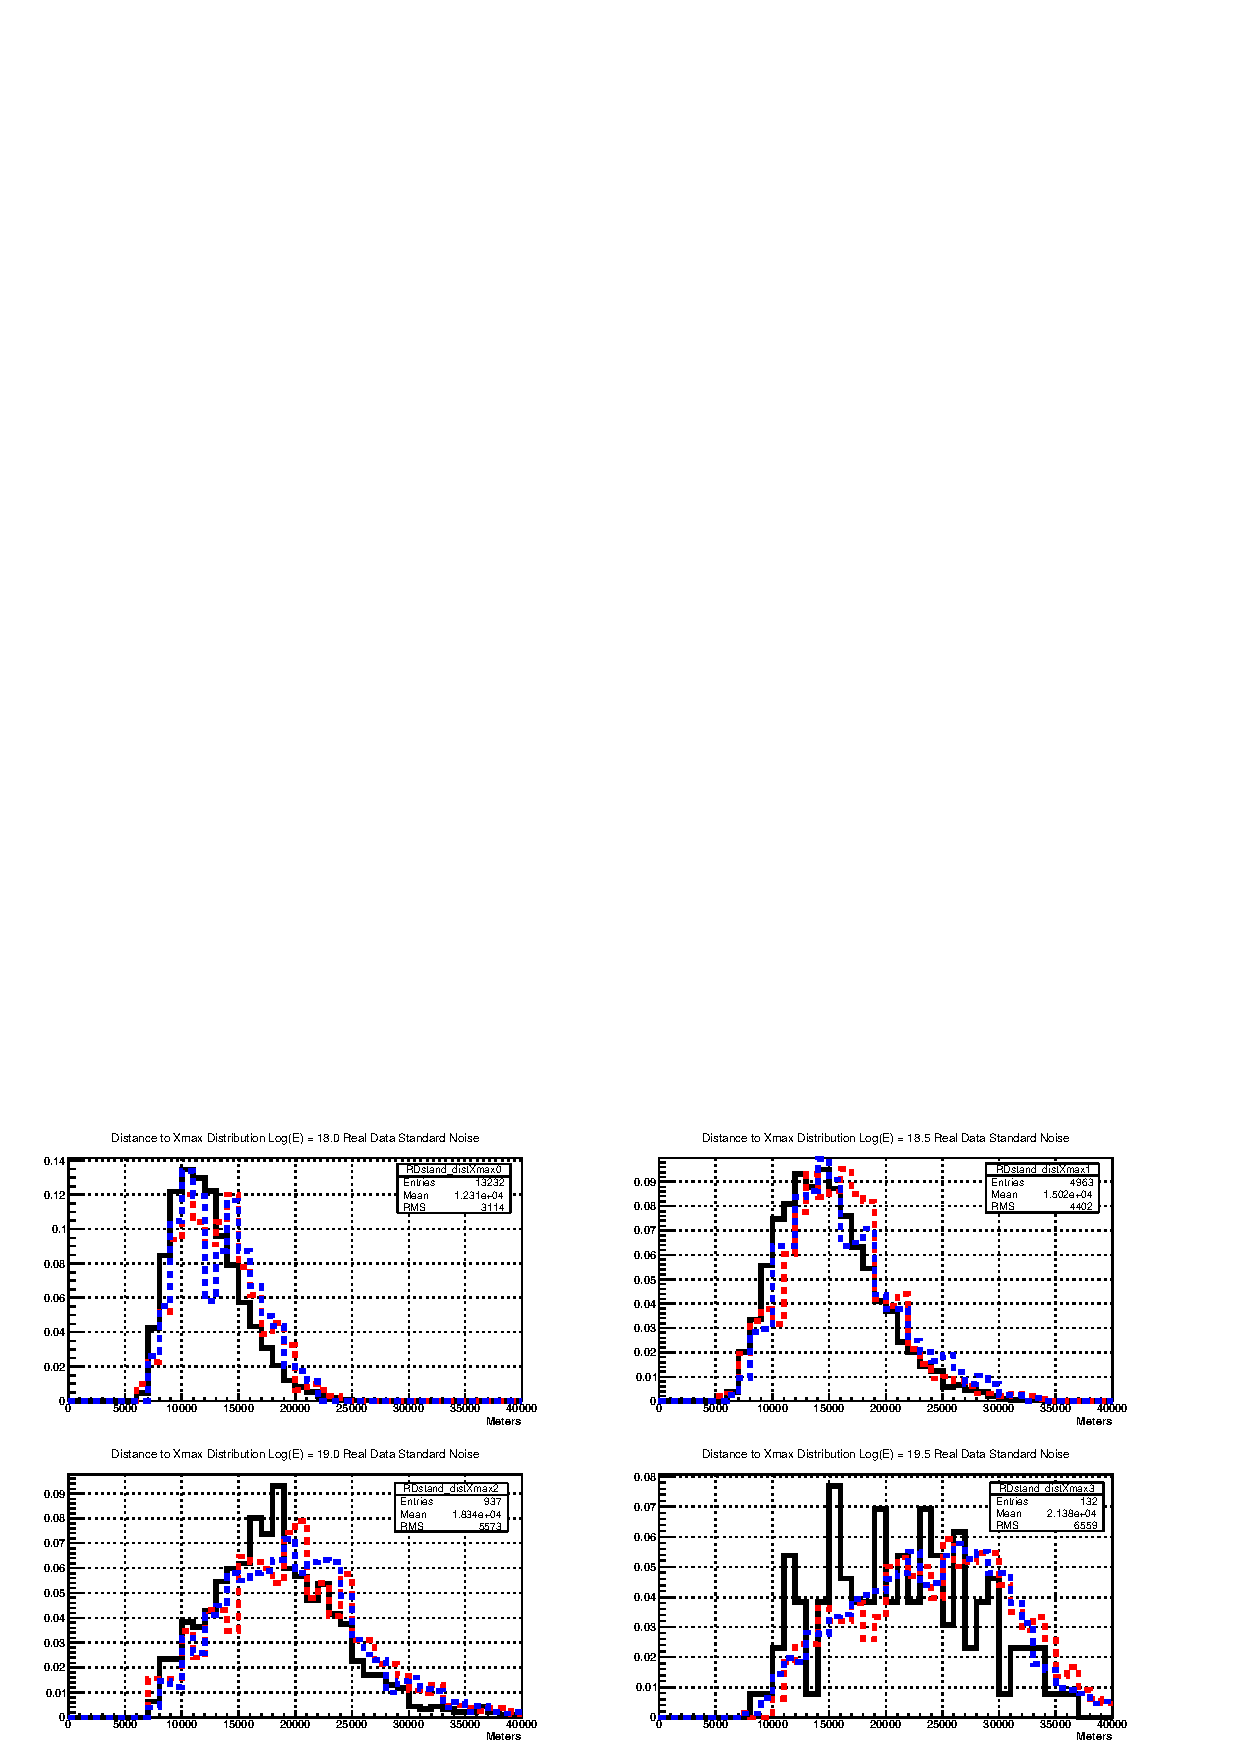
\includegraphics[width=\textwidth]{chapters/graphs/SelectionEff/RealDataAndSim_DistToXmaxDistComp.pdf}
\caption{Distribution of Distance to Xmax with Real Data and simulation of proton and iron showers.}
\end{figure}


\begin{figure}
\centering
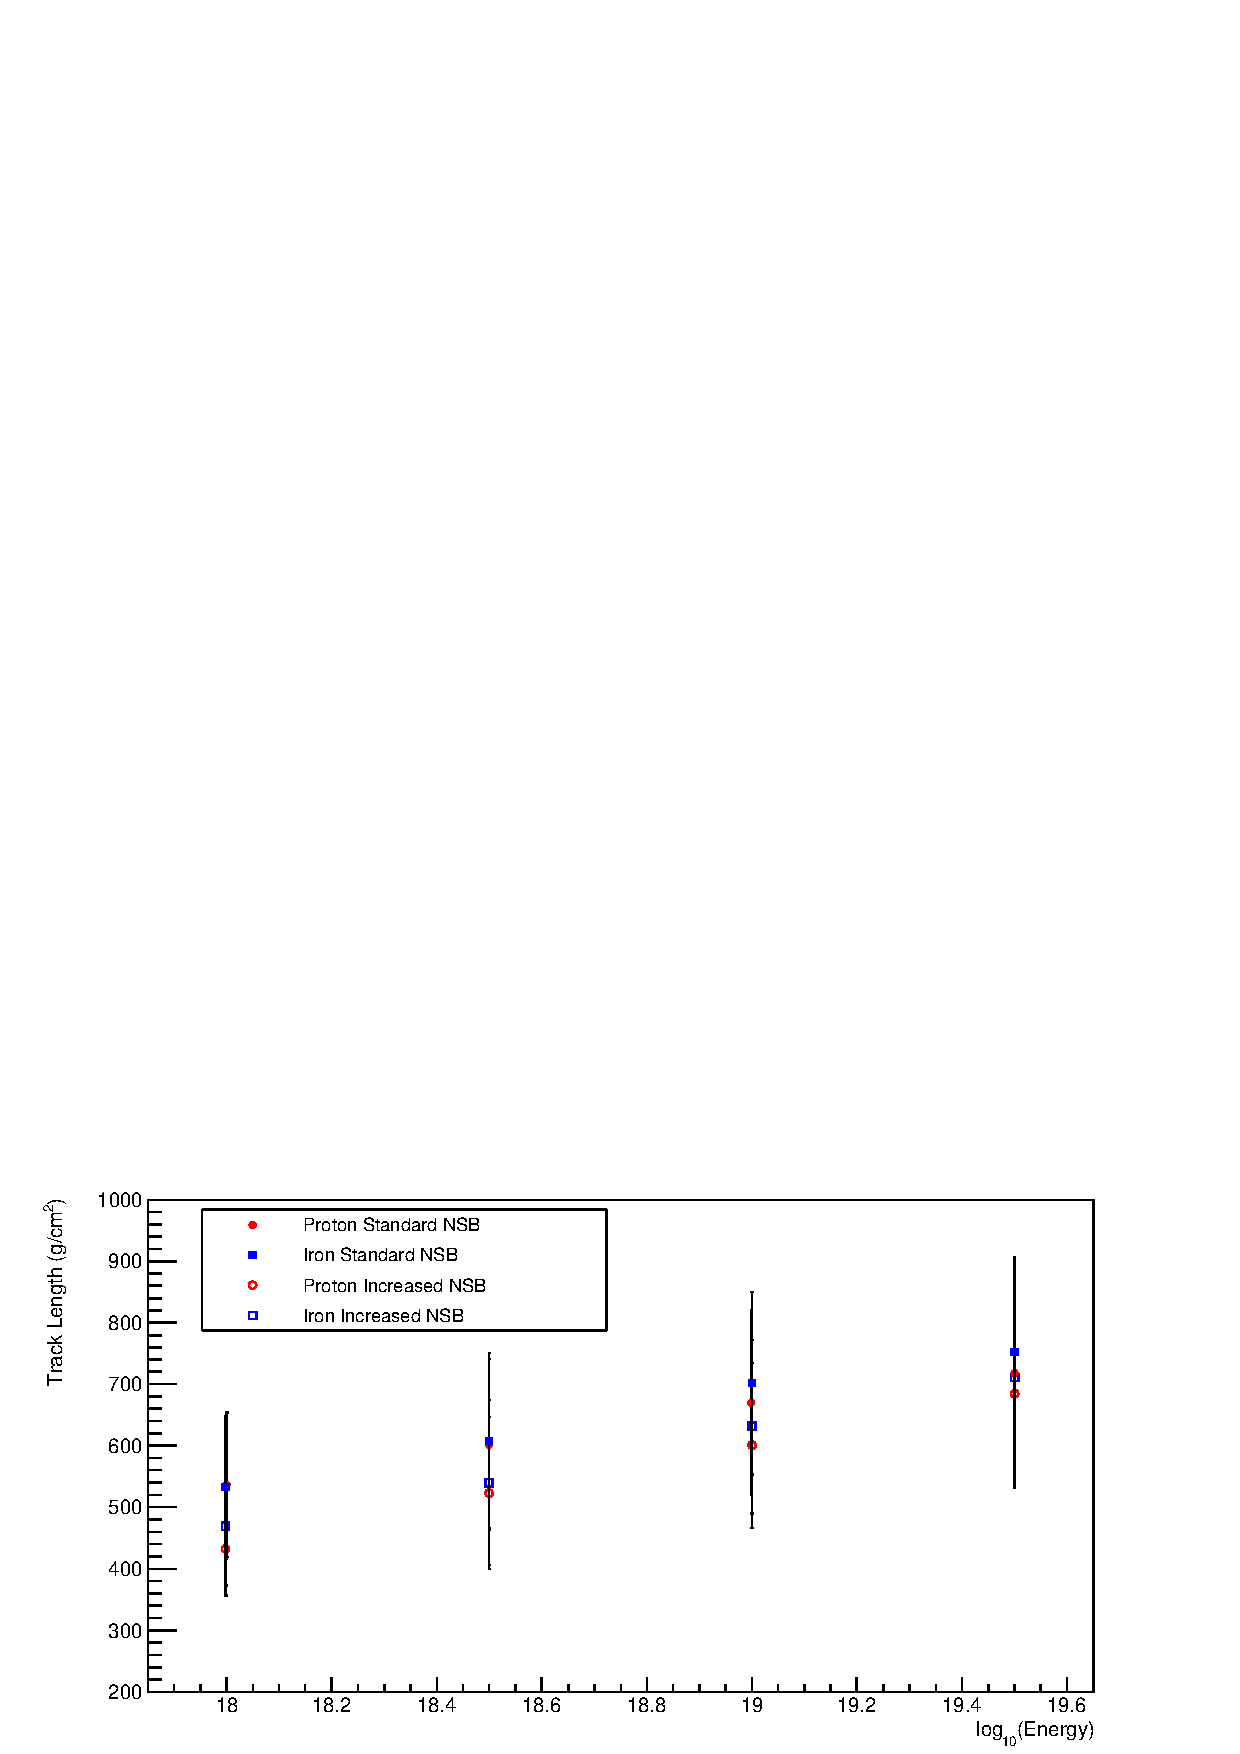
\includegraphics[width=\textwidth]{chapters/graphs/SelectionEff/Simulation_TrackLength_Comb_StandANdIncreasedNSB.pdf}
\caption{Track length using simulation of proton and iron CONEX showers.} \label{fig:TrackLength_Sim}
\end{figure}
\subsection{Discussion}

\section{Conclusion/Summary}
\chapter{Quantifying Characteristics of the FD PMT}\label{Ch:PMTCharacter}

Characterising the PMT at 600V and 900V
\begin{itemize}
\item Using the characteristics of the PMT at 900V as a baseline
\item Measure linearity
\item ND filters bs Two LED method
\item Pulse shape?
\item temperature effects
\item dark noise?
\end{itemize}
\chapter[Computer Simulation of FD PMT]{\centering Computer Simulation of FD PMT \\}\label{Ch:CompSimPMT}

Simulating the FD PMT under differing NSB and for different reasons.
\begin{itemize}
\item Theoretical value for Gain Variance
\item PMT Gain Variance
\item Show both for flat distribution and Gaussian variations for dynodes
\item Results
\item FD FLT under increased NSB
\item Kv simulation under increased NSB?
\end{itemize}

\begin{figure}
\centering
\begin{subfigure}[b]{0.44\textwidth}
\adjincludegraphics[width=\textwidth, trim={0 0 0 {0.08\height}}, clip]{chapters/graphs/PMTsimulation/ElectronsLeaving_PoissonFit_Dynode1_5e4.pdf}
\caption{Distribution of simulated electrons leaving dynode 1. The red line is a fitted Poisson distribution.}
\end{subfigure}
\hspace{3mm}
\begin{subfigure}[b]{0.44\textwidth}
\adjincludegraphics[width=\textwidth, trim={0 0 0 {0.08\height}}, clip]{chapters/graphs/PMTsimulation/ElectronsLeaving_Dynode2_5e4.pdf}
\caption{Distribution of simulated electrons leaving dynode 2. The red line is a fitted Gaussian distribution.}
\end{subfigure}

\vspace{3mm}

\begin{subfigure}[b]{0.44\textwidth}
\adjincludegraphics[width=\textwidth, trim={0 0 0 {0.08\height}}, clip]{chapters/graphs/PMTsimulation/ElectronsLeaving_Dynode3_5e4.pdf}
\caption{Distribution of simulated electrons leaving dynode 3. The red line is a fitted Poisson distribution.}
\end{subfigure}
\hspace{3mm}
\begin{subfigure}[b]{0.44\textwidth}
\adjincludegraphics[width=\textwidth, trim={0 0 0 {0.08\height}}, clip]{chapters/graphs/PMTsimulation/ElectronsLeaving_Dynode4_5e4.pdf}
\caption{Distribution of simulated electrons leaving dynode 4. The red line is a fitted Gaussian distribution.}
\end{subfigure}

\vspace{3mm}

\begin{subfigure}[b]{0.44\textwidth}
\adjincludegraphics[width=\textwidth, trim={0 0 0 {0.08\height}}, clip]{chapters/graphs/PMTsimulation/ElectronsLeaving_Dynode5_5e4.pdf}
\caption{Distribution of simulated electrons leaving dynode 5. The red line is a fitted Poisson distribution.}
\end{subfigure}
\hspace{3mm}
\begin{subfigure}[b]{0.44\textwidth}
\adjincludegraphics[width=\textwidth, trim={0 0 0 {0.08\height}}, clip]{chapters/graphs/PMTsimulation/ElectronsLeaving_Dynode6_5e4.pdf}
\caption{Distribution of simulated electrons leaving dynode 6. The red line is a fitted Gaussian distribution.}
\end{subfigure}

\vspace{3mm}

\begin{subfigure}[b]{0.44\textwidth}
\adjincludegraphics[width=\textwidth, trim={0 0 0 {0.08\height}}, clip]{chapters/graphs/PMTsimulation/ElectronsLeaving_Dynode7_5e4.pdf}
\caption{Distribution of simulated electrons leaving dynode 7. The red line is a fitted Poisson distribution.}
\end{subfigure}
\hspace{3mm}
\begin{subfigure}[b]{0.44\textwidth}
\adjincludegraphics[width=\textwidth, trim={0 0 0 {0.08\height}}, clip]{chapters/graphs/PMTsimulation/ElectronsLeaving_Dynode8_5e4.pdf}
\caption{Distribution of simulated electrons leaving dynode 8. The red line is a fitted Gaussian distribution.}
\end{subfigure}
\end{figure}

\begin{figure}
\centering
\begin{subfigure}[b]{0.44\textwidth}
\adjincludegraphics[width=\textwidth, trim={0 0 0 {0.08\height}}, clip]{chapters/graphs/PMTsimulation/PMTsim_1PE_TypeC_DynodeSigm0_5e5.pdf}
\caption{Simulated observed signal from PMT anode with 8 stages and gain of 5 $\times \ 10^5$. Poisson fluctuations at each stage only. No each Gaussian broadening at any dynode.}
\end{subfigure}
\hspace{3mm}
\begin{subfigure}[b]{0.44\textwidth}
\adjincludegraphics[width=\textwidth, trim={0 0 0 {0.08\height}}, clip]{chapters/graphs/PMTsimulation/PMTsim_1PE_TypeC_DynodeSigm0_1_5e5.pdf}
\caption{Simulated observed signal from PMT anode with 8 stages and gain of 5 $\times \ 10^5$. Poisson fluctuations at each stage only. Added Gaussian braodening at each dynode of 10\%.}
\end{subfigure}

\vspace{3mm}

\begin{subfigure}[b]{0.44\textwidth}
\adjincludegraphics[width=\textwidth, trim={0 0 0 {0.08\height}}, clip]{chapters/graphs/PMTsimulation/PMTsim_1PE_TypeC_DynodeSigm0_2_5e5.pdf}
\caption{Simulated observed signal from PMT anode with 8 stages and gain of 5 $\times \ 10^5$. Poisson fluctuations at each stage only. Added Gaussian braodening at each dynode of 20\%.}
\end{subfigure}
\hspace{3mm}
\begin{subfigure}[b]{0.44\textwidth}
\adjincludegraphics[width=\textwidth, trim={0 0 0 {0.08\height}}, clip]{chapters/graphs/PMTsimulation/PMTsim_1PE_TypeC_DynodeSigm0_3_5e5.pdf}
\caption{Simulated observed signal from PMT anode with 8 stages and gain of 5 $\times \ 10^5$. Poisson fluctuations at each stage only. Added Gaussian braodening at each dynode of 30\%.}
\end{subfigure}

\vspace{3mm}

\begin{subfigure}[b]{0.44\textwidth}
\adjincludegraphics[width=\textwidth, trim={0 0 0 {0.08\height}}, clip]{chapters/graphs/PMTsimulation/PMTsim_1PE_TypeC_DynodeSigm0_4_5e5.pdf}
\caption{Simulated observed signal from PMT anode with 8 stages and gain of 5 $\times \ 10^5$. Poisson fluctuations at each stage only. Added Gaussian braodening at each dynode of 40\%.}
\end{subfigure}
\hspace{3mm}
\begin{subfigure}[b]{0.44\textwidth}
\adjincludegraphics[width=\textwidth, trim={0 0 0 {0.08\height}}, clip]{chapters/graphs/PMTsimulation/PMTsim_1PE_TypeC_DynodeSigm0_5_5e5.pdf}
\caption{Simulated observed signal from PMT anode with 8 stages and gain of 5 $\times \ 10^5$. Poisson fluctuations at each stage only. Added Gaussian braodening at each dynode of 50\%.}
\end{subfigure}
\end{figure}

\begin{figure}
\centering
\begin{subfigure}[b]{0.44\textwidth}
\adjincludegraphics[width=\textwidth, trim={0 0 0 {0.08\height}}, clip]{chapters/graphs/PMTsimulation/PMTsim_1PE_TypeC_DynodeSigm0_5e4.pdf}
\caption{Simulated observed signal from PMT anode with 8 stages and gain of 5 $\times \ 10^4$. Poisson fluctuations at each stage only. No each Gaussian broadening at any dynode.}
\end{subfigure}
\hspace{3mm}
\begin{subfigure}[b]{0.44\textwidth}
\adjincludegraphics[width=\textwidth, trim={0 0 0 {0.08\height}}, clip]{chapters/graphs/PMTsimulation/PMTsim_1PE_TypeC_DynodeSigm0_1_5e4.pdf}
\caption{Simulated observed signal from PMT anode with 8 stages and gain of 5 $\times \ 10^4$. Poisson fluctuations at each stage only. Added Gaussian braodening at each dynode of 10\%.}
\end{subfigure}

\vspace{3mm}

\begin{subfigure}[b]{0.44\textwidth}
\adjincludegraphics[width=\textwidth, trim={0 0 0 {0.08\height}}, clip]{chapters/graphs/PMTsimulation/PMTsim_1PE_TypeC_DynodeSigm0_2_5e4.pdf}
\caption{Simulated observed signal from PMT anode with 8 stages and gain of 5 $\times \ 10^4$. Poisson fluctuations at each stage only. Added Gaussian braodening at each dynode of 20\%.}
\end{subfigure}
\hspace{3mm}
\begin{subfigure}[b]{0.44\textwidth}
\adjincludegraphics[width=\textwidth, trim={0 0 0 {0.08\height}}, clip]{chapters/graphs/PMTsimulation/PMTsim_1PE_TypeC_DynodeSigm0_3_5e4.pdf}
\caption{Simulated observed signal from PMT anode with 8 stages and gain of 5 $\times \ 10^4$. Poisson fluctuations at each stage only. Added Gaussian braodening at each dynode of 30\%.}
\end{subfigure}

\vspace{3mm}

\begin{subfigure}[b]{0.44\textwidth}
\adjincludegraphics[width=\textwidth, trim={0 0 0 {0.08\height}}, clip]{chapters/graphs/PMTsimulation/PMTsim_1PE_TypeC_DynodeSigm0_4_5e4.pdf}
\caption{Simulated observed signal from PMT anode with 8 stages and gain of 5 $\times \ 10^4$. Poisson fluctuations at each stage only. Added Gaussian braodening at each dynode of 40\%.}
\end{subfigure}
\hspace{3mm}
\begin{subfigure}[b]{0.44\textwidth}
\adjincludegraphics[width=\textwidth, trim={0 0 0 {0.08\height}}, clip]{chapters/graphs/PMTsimulation/PMTsim_1PE_TypeC_DynodeSigm0_5_5e4.pdf}
\caption{Simulated observed signal from PMT anode with 8 stages and gain of 5 $\times \ 10^4$. Poisson fluctuations at each stage only. Added Gaussian braodening at each dynode of 50\%.}
\end{subfigure}
\end{figure}

\begin{figure}
\centering
\begin{subfigure}[b]{0.44\textwidth}
\adjincludegraphics[width=\textwidth, trim={0 0 0 {0.08\height}}, clip]{chapters/graphs/PMTsimulation/PMTsim_1PE_TypeC_DynodeSigm0_5e3.pdf}
\caption{Simulated observed signal from PMT anode with 8 stages and gain of 5 $\times \ 10^3$. Poisson fluctuations at each stage only. No each Gaussian broadening at any dynode.}
\end{subfigure}
\hspace{3mm}
\begin{subfigure}[b]{0.44\textwidth}
\adjincludegraphics[width=\textwidth, trim={0 0 0 {0.08\height}}, clip]{chapters/graphs/PMTsimulation/PMTsim_1PE_TypeC_DynodeSigm0_1_5e3.pdf}
\caption{Simulated observed signal from PMT anode with 8 stages and gain of 5 $\times \ 10^3$. Poisson fluctuations at each stage only. Added Gaussian braodening at each dynode of 10\%.}
\end{subfigure}

\vspace{3mm}

\begin{subfigure}[b]{0.44\textwidth}
\adjincludegraphics[width=\textwidth, trim={0 0 0 {0.08\height}}, clip]{chapters/graphs/PMTsimulation/PMTsim_1PE_TypeC_DynodeSigm0_2_5e3.pdf}
\caption{Simulated observed signal from PMT anode with 8 stages and gain of 5 $\times \ 10^3$. Poisson fluctuations at each stage only. Added Gaussian braodening at each dynode of 20\%.}
\end{subfigure}
\hspace{3mm}
\begin{subfigure}[b]{0.44\textwidth}
\adjincludegraphics[width=\textwidth, trim={0 0 0 {0.08\height}}, clip]{chapters/graphs/PMTsimulation/PMTsim_1PE_TypeC_DynodeSigm0_3_5e3.pdf}
\caption{Simulated observed signal from PMT anode with 8 stages and gain of 5 $\times \ 10^3$. Poisson fluctuations at each stage only. Added Gaussian braodening at each dynode of 30\%.}
\end{subfigure}

\vspace{3mm}

\begin{subfigure}[b]{0.44\textwidth}
\adjincludegraphics[width=\textwidth, trim={0 0 0 {0.08\height}}, clip]{chapters/graphs/PMTsimulation/PMTsim_1PE_TypeC_DynodeSigm0_4_5e3.pdf}
\caption{Simulated observed signal from PMT anode with 8 stages and gain of 5 $\times \ 10^3$. Poisson fluctuations at each stage only. Added Gaussian braodening at each dynode of 40\%.}
\end{subfigure}
\hspace{3mm}
\begin{subfigure}[b]{0.44\textwidth}
\adjincludegraphics[width=\textwidth, trim={0 0 0 {0.08\height}}, clip]{chapters/graphs/PMTsimulation/PMTsim_1PE_TypeC_DynodeSigm0_5_5e3.pdf}
\caption{Simulated observed signal from PMT anode with 8 stages and gain of 5 $\times \ 10^3$. Poisson fluctuations at each stage only. Added Gaussian braodening at each dynode of 50\%.}
\end{subfigure}
\end{figure}

\begin{figure}
\centering
\begin{subfigure}[b]{0.44\textwidth}
\adjincludegraphics[width=\textwidth, trim={0 0 0 {0.08\height}}, clip]{chapters/graphs/PMTsimulation/FLT_simulation_2_71pePER100ns.pdf}
\caption{FLT simulation with NSB of 2.71 pe / 100ns.}
\end{subfigure}
\hspace{3mm}
\begin{subfigure}[b]{0.44\textwidth}
\adjincludegraphics[width=\textwidth, trim={0 0 0 {0.08\height}}, clip]{chapters/graphs/PMTsimulation/FLT_simulation_6_60pePER100ns.pdf}
\caption{FLT simulation with NSB of 6.60 pe / 100ns.}
\end{subfigure}

\vspace{3mm}

\begin{subfigure}[b]{0.44\textwidth}
\adjincludegraphics[width=\textwidth, trim={0 0 0 {0.08\height}}, clip]{chapters/graphs/PMTsimulation/FLT_simulation_46_8pePER100ns.pdf}
\caption{FLT simulation with NSB of 46.8 pe / 100ns.}
\end{subfigure}
\hspace{3mm}
\begin{subfigure}[b]{0.44\textwidth}
\adjincludegraphics[width=\textwidth, trim={0 0 0 {0.08\height}}, clip]{chapters/graphs/PMTsimulation/FLT_simulation_65_8pePER100ns.pdf}
\caption{FLT simulation with NSB of 65.8 pe / 100ns.}
\end{subfigure}

\vspace{3mm}
\begin{subfigure}[b]{0.44\textwidth}
\adjincludegraphics[width=\textwidth, trim={0 0 0 {0.08\height}}, clip]{chapters/graphs/PMTsimulation/FLT_simulation_263pePER100ns.pdf}
\caption{FLT simulation with NSB of 263 pe / 100ns.}
\end{subfigure}
\hspace{3mm}
\begin{subfigure}[b]{0.44\textwidth}
\adjincludegraphics[width=\textwidth, trim={0 0 0 {0.08\height}}, clip]{chapters/graphs/PMTsimulation/FLT_simulation_657pePER100ns.pdf}
\caption{FLT simulation with NSB of 657 pe / 100ns.}
\end{subfigure}
\end{figure}
\chapter[Measuring FD PMT Gain Variance with CalA Data]{\centering Measuring FD PMT Gain Variance with CalA Data \\}\label{Ch:GainVariance}

Measuring Gain Variance of FD PMT with CalA Data
\begin{itemize}
\item Measuring Gain Variance in the lab did not work. Equipment was not sensitive enough to the low current.
\item There was issues with calibrating the LED light source with another PMT (QE curve and wavelength response not the same?)
\item Using Low/Standard measurements of CalA to find Gain Variance Ratio
\item Two different methods
\item Bootstrap method to find uncertainties on Method 2
\end{itemize}

\section{Using CalA to measure relative changes in Gain Variance}

Using CalA data from the FD telescopes to measure the relative changes in PMT  gain variance as the gain is changed by a factor of 10. CalA data is calibration data used to monitor any changes in PMT gain as a function of time. CalA is performed at the beginning and end of a nightly observation done with the FDs. Pulses from a monitored light source are piped to point at the camera. There are 50 pulses sent with a width of approximately 60 $\mu$s.

\textbf{show image of CalA pulse}

One of the values that can be calculated from the CalA is a value denoted K$_{\mathrm{V}}$. K$_{\mathrm{V}}$ is calculated via:
\begin{equation}
\mathrm{K}_{\mathrm{V}} = \frac{\mathrm{Mean}}{\mathrm{Sigma}^2} = \frac{10}{2 \times \mathrm{G} (1 + \mathrm{V}_{\mathrm{G}}) \times \mathrm{F}}
\end{equation}
Mean is the average ADC count of the observed CalA pulse seen the FD pixel, sigma$^2$ is the variance calculated around fit to the signal in ADC$^2$. The signal has a slope due to the effects of a capacitor used to remove the DC component of the signal. The slope is proportional to the time constant of the capacitor employed. G is the PMT gain, F is the noise equivalent bandwidth (Hz) and V$_{\mathrm{G}}$ is the PMT gain variance.

The absolute value of the gain variance cannot be found but using K$_{\mathrm{V}}$ a relative change can be found. This is useful for the collaboration simulations as a Gain variance is coded for the PMT at standard voltage settings. Finding out the relative change in gain variance would be useful to be used for simulations of the FD PMTs at a lower voltage settings (IE. 600V).

The method used to measure the ratio in gain variance is to take the calculated means and sigmas from the pulses and then find a ratio between the K$_{\mathrm{V}}$ and Gains at the two different voltage settings.
\begin{eqnarray}
\mathrm{K} = \frac{\mathrm{Mean}}{\mathrm{Sigma}^2} &=& \frac{10}{2 \times \mathrm{G} (1 + \mathrm{V}_{\mathrm{G}}) \times \mathrm{F}} \\ 
\frac{\left(\mathrm{K}_{\mathrm{V}}\right)_{\mathrm{Low}}}{\left(\mathrm{K}_{\mathrm{V}}\right)_{\mathrm{Stand}}} &=& \frac{\mathrm{Mean}_{\mathrm{Low}}}{\mathrm{Sigma}^2_{\mathrm{Low}}} \div \frac{\mathrm{Mean}_{\mathrm{Stand}}}{\mathrm{Sigma}^2_{\mathrm{Stand}}} \\ 
\frac{\mathrm{Mean}_{\mathrm{Low}}}{\mathrm{Sigma}^2_{\mathrm{Low}}} \div \frac{\mathrm{Mean}_{\mathrm{Stand}}}{\mathrm{Sigma}^2_{\mathrm{Stand}}} &=& \frac{\mathrm{G}_{\mathrm{Stand}} (1 + \mathrm{V}_{\mathrm{G}})_{\mathrm{Stand}}}{\mathrm{G}_{\mathrm{Low}} (1 + \mathrm{V}_{\mathrm{G}})_{\mathrm{Low}}} \\
\frac{\mathrm{G}_{\mathrm{Stand}}}{\mathrm{G}_{\mathrm{Low}}} &=& \frac{\mathrm{Mean}_{\mathrm{Stand}}}{\mathrm{Mean}_{\mathrm{Low}}} \\
\frac{(1 + \mathrm{V}_{\mathrm{G}})_{\mathrm{Low}}}{(1 + \mathrm{V}_{\mathrm{G}})_{\mathrm{Stand}}} &=& \frac{\mathrm{Sigma}^2_{\mathrm{Low}} \times \mathrm{Mean}^2_{\mathrm{Stand}}}{\mathrm{Sigma}^2_{\mathrm{Stand}} \times \mathrm{Mean}^2_{\mathrm{Low}}}
\end{eqnarray}

\section{Electronic Noise}

Investigated the consistency of the electronic noise across a set of 50 CalA traces. The consistency was looked as there is only about 140 bins of noise before the signal pulse start. Therefore finding an accurate mean and variance of the electronic noise on an individual pulse is difficult. An accurate measurement of the electronic noise mean and variance was required as the measured gain variance ratio was only a few percent.

\textbf{Need to show electronic noise as function of time.}

An example of a pixel electronic noise trace is shown in Fig. \ref{}. It can be seen in this figure that stitching all of the noise bins from the 50 traces is remarkably stable. This result allows for all the noise for a single PMT pixel to be place into a histogram to find a more accurate value for the mean and variance.

\begin{figure} % Electronic Noise Distribution
\centering
\begin{subfigure}[b]{0.95\textwidth}
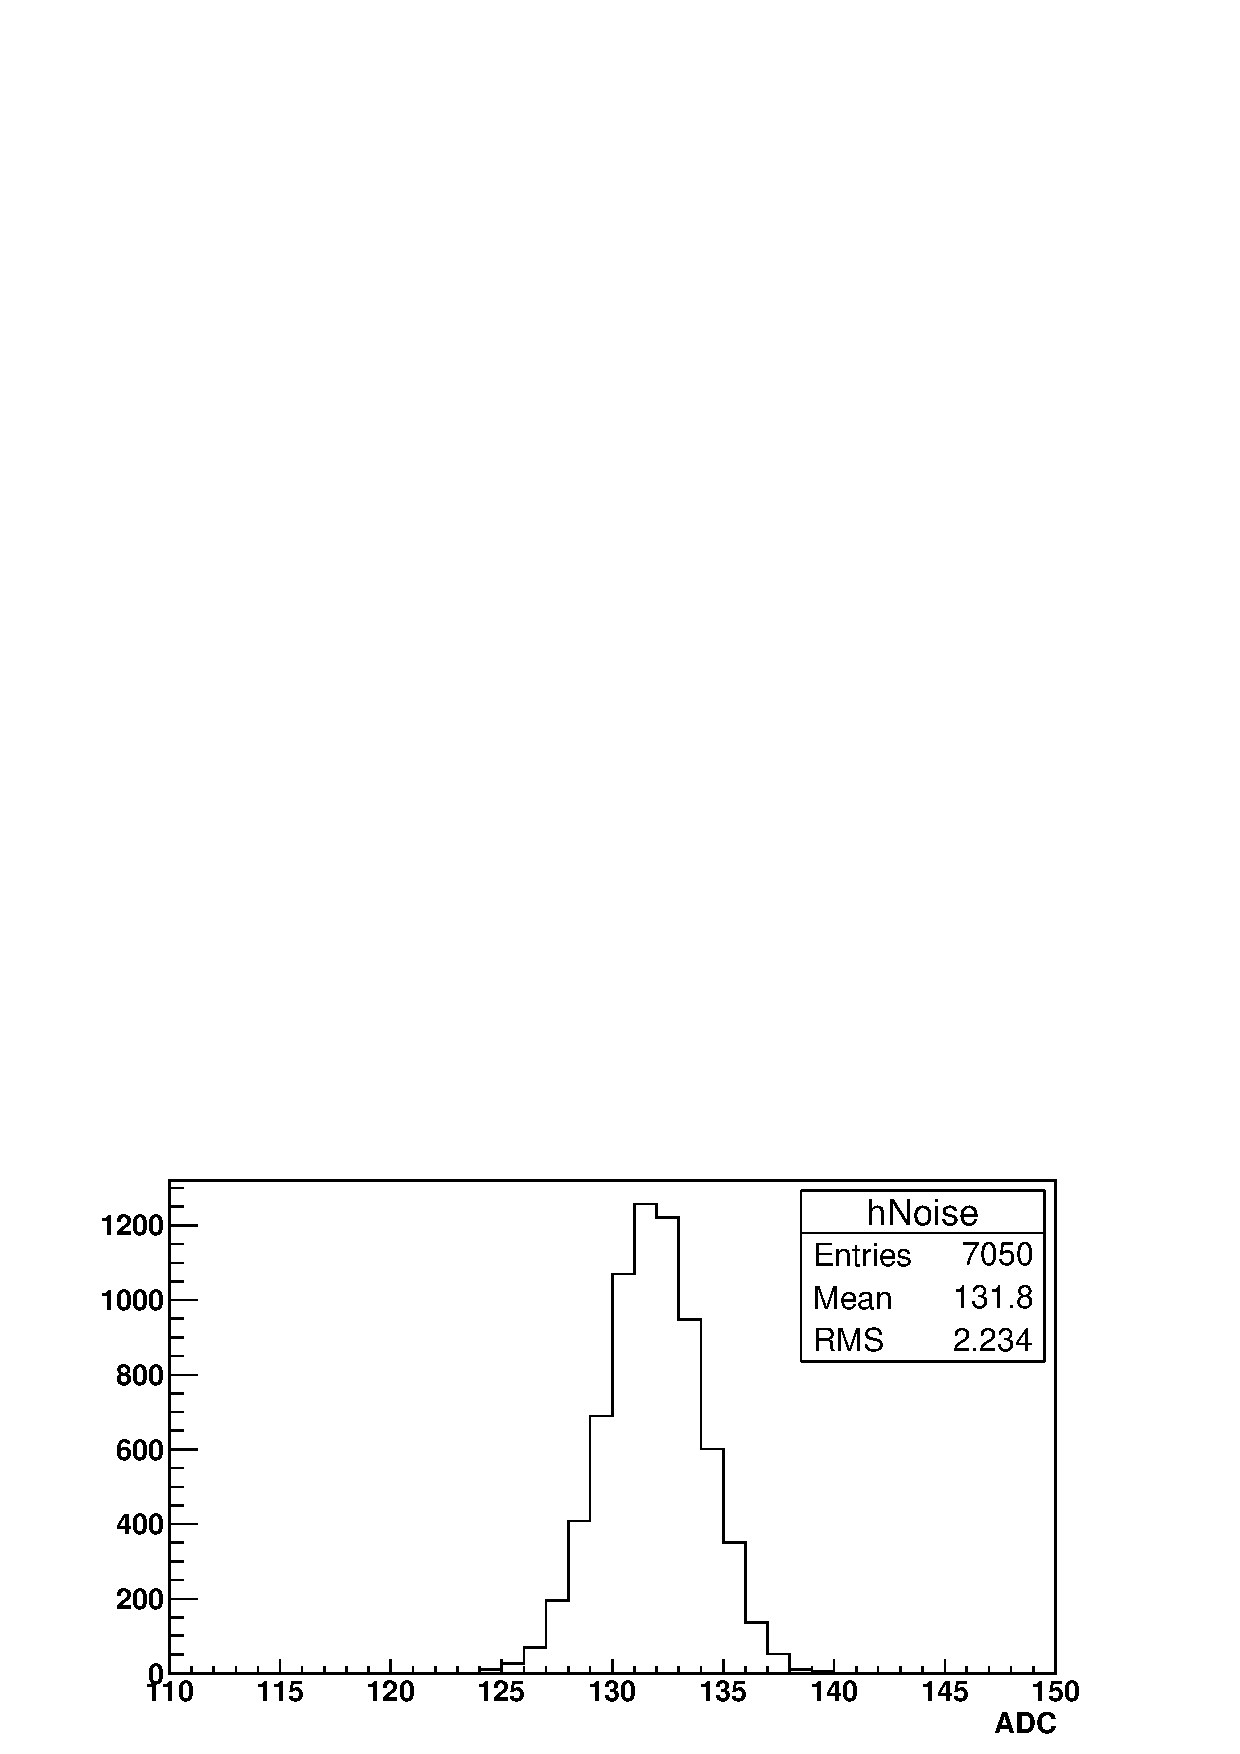
\includegraphics[width=\textwidth]{chapters/graphs/GainVarsMeas/LL_m04_2016-06-11/example_NoiseHist1.pdf}
\caption{}
\end{subfigure}
\vspace{3mm}
\begin{subfigure}[b]{0.95\textwidth}
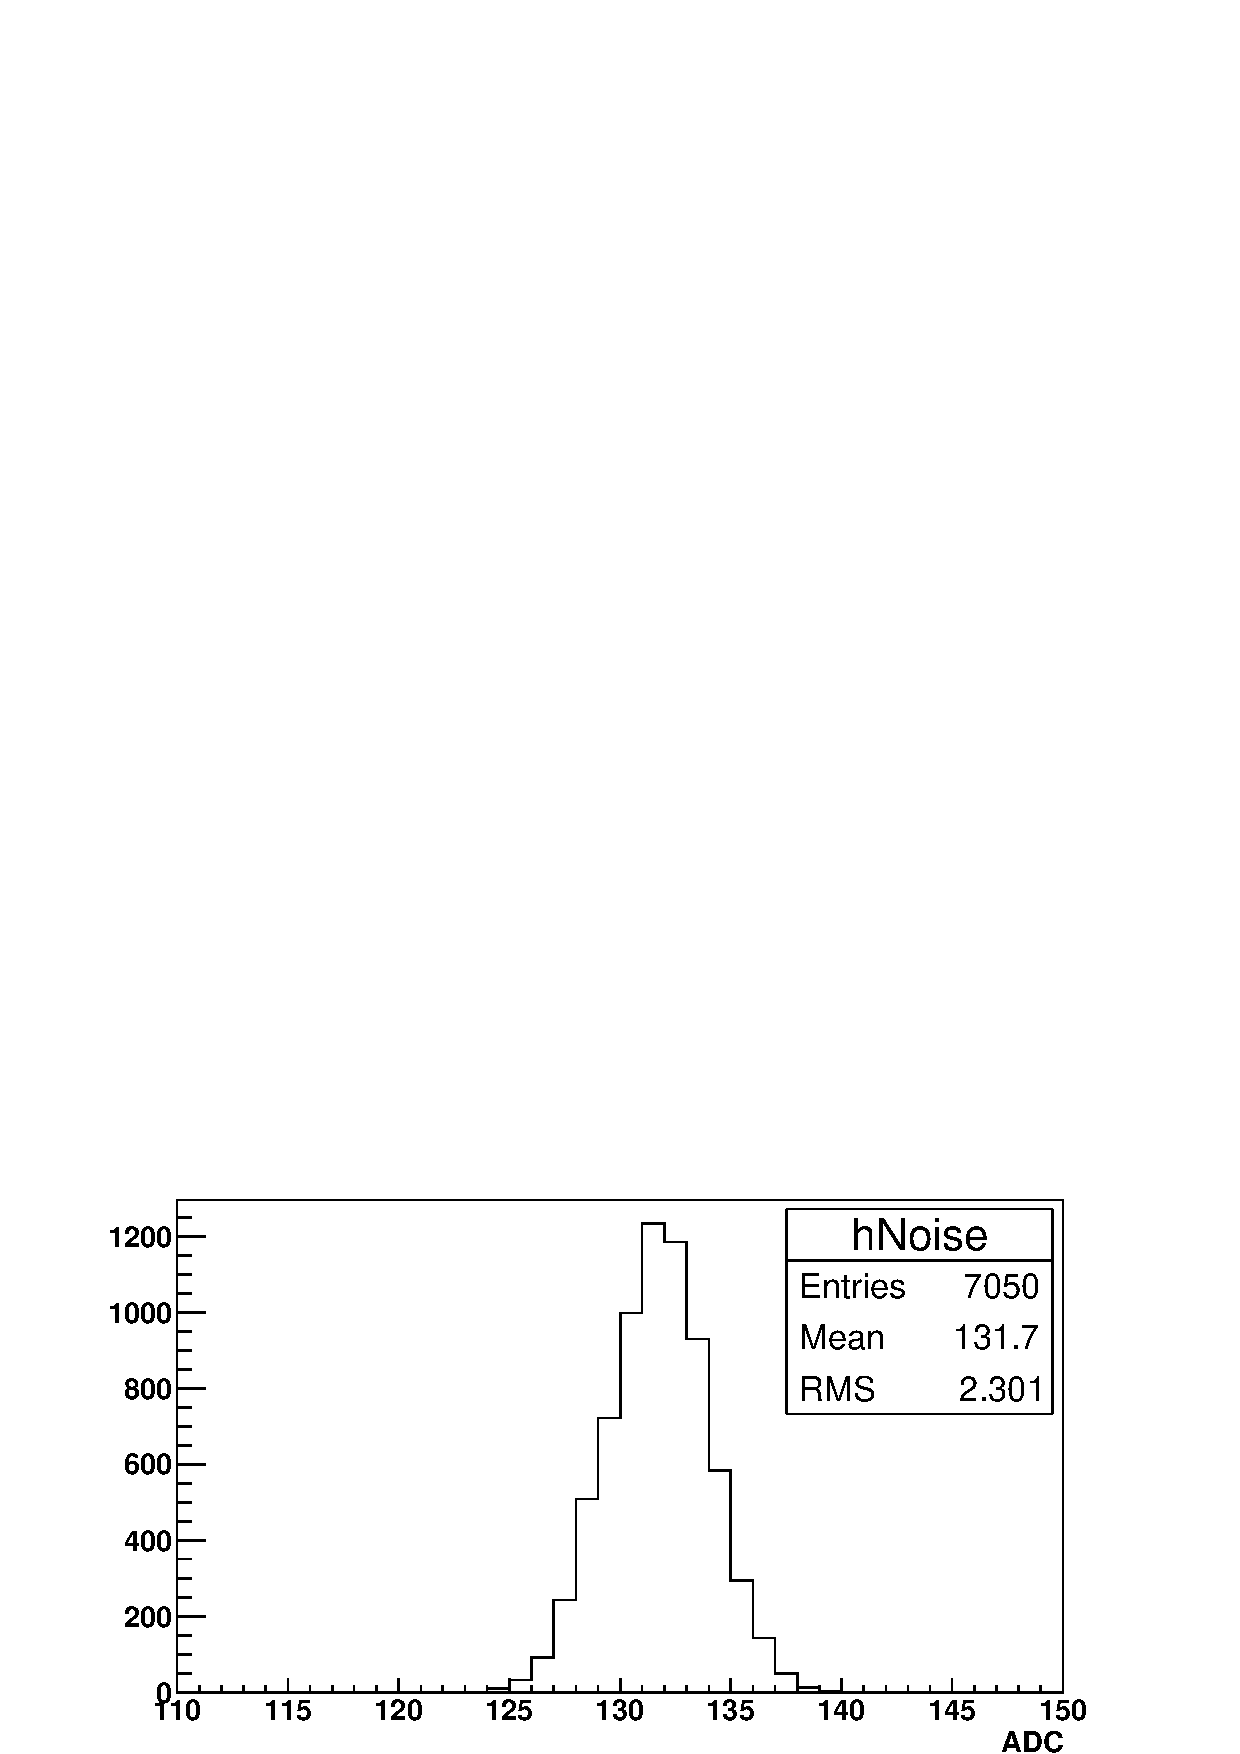
\includegraphics[width=\textwidth]{chapters/graphs/GainVarsMeas/LL_m04_2016-06-11/example_NoiseHist2.pdf}
\caption{}
\end{subfigure}
\caption{Sample of the observed electronic noise observed for a single pixel within Los Leones telescope 4.}
\end{figure}

\section{Pairs Method}

For both standard and reduced voltage settings 50 sets of pulses are recorded for the CalA analysis. The pair method involves taking single CalA shots from standard and lower voltage settings and fitting an exponential to the signal. The fitted exponential is used to find the mean value at the top of the signal and the variance around the fit. For each pixel 50 values for the Gain Variance ratio is found and this is repeated for the 440 pixels within the FD telescope.

Fig. \ref{fig:CalAMeanADC_Pairs} shows the average ADC count found across a camera for a FD telescope. The pattern follow how the camera is illuminated by the LED pointing at the camera. It shows that the spot is brightness in the middle and the intensity drops off towards the edges \textbf{need to add in diagram of labelled pixel no. across a FD camera}. There are uncertainties on the averages but are smaller then the displayed points. The variance measured in Fig. \ref{fig:CalAVarsADC_Pairs} shows an expected pattern too. The variance is proportional to the mean

\subsection{Results}

\begin{figure} % Mean Plot
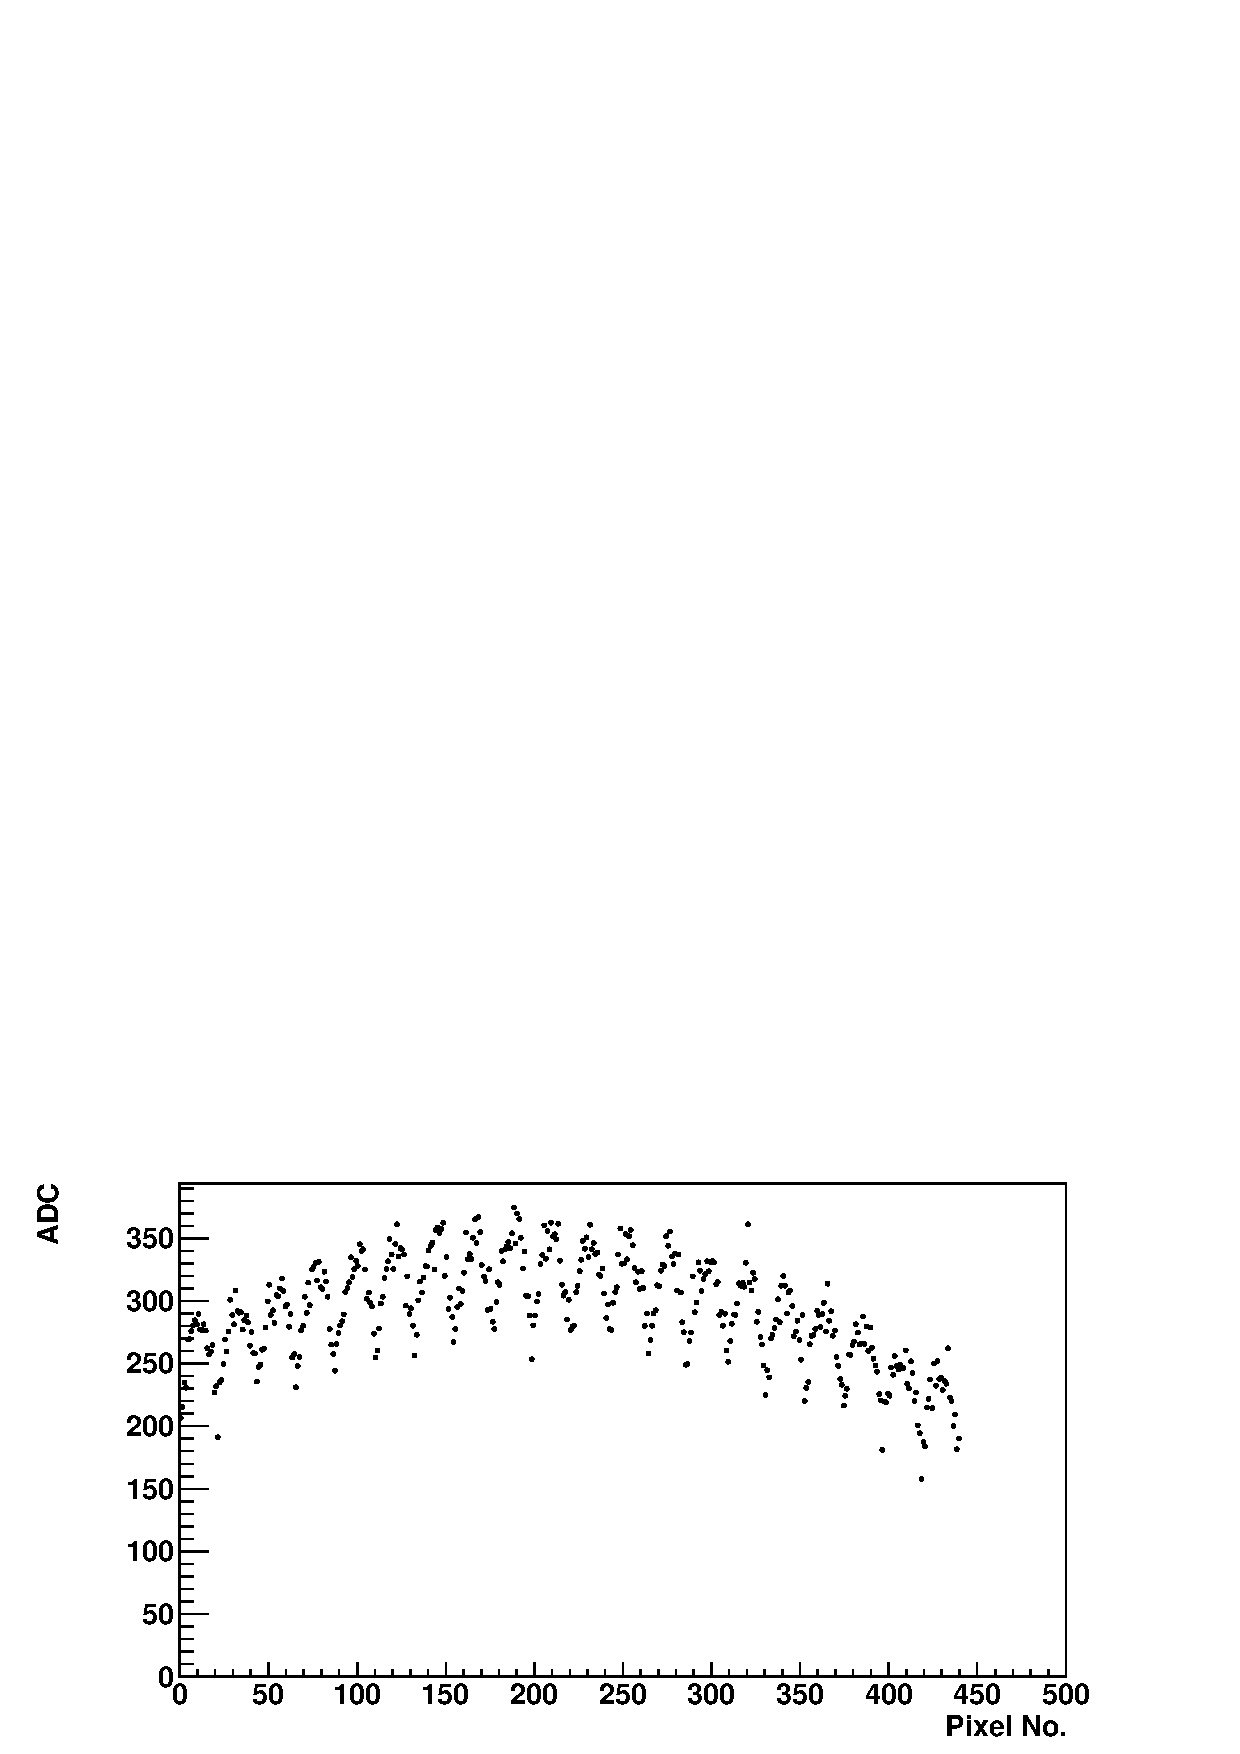
\includegraphics[width=\textwidth]{chapters/graphs/GainVarsMeas/LL_m04_2016-06-11/Set0and2/meanHist_StandHV_Pairs_set0and2.pdf}
\caption{}
\vspace{3mm}
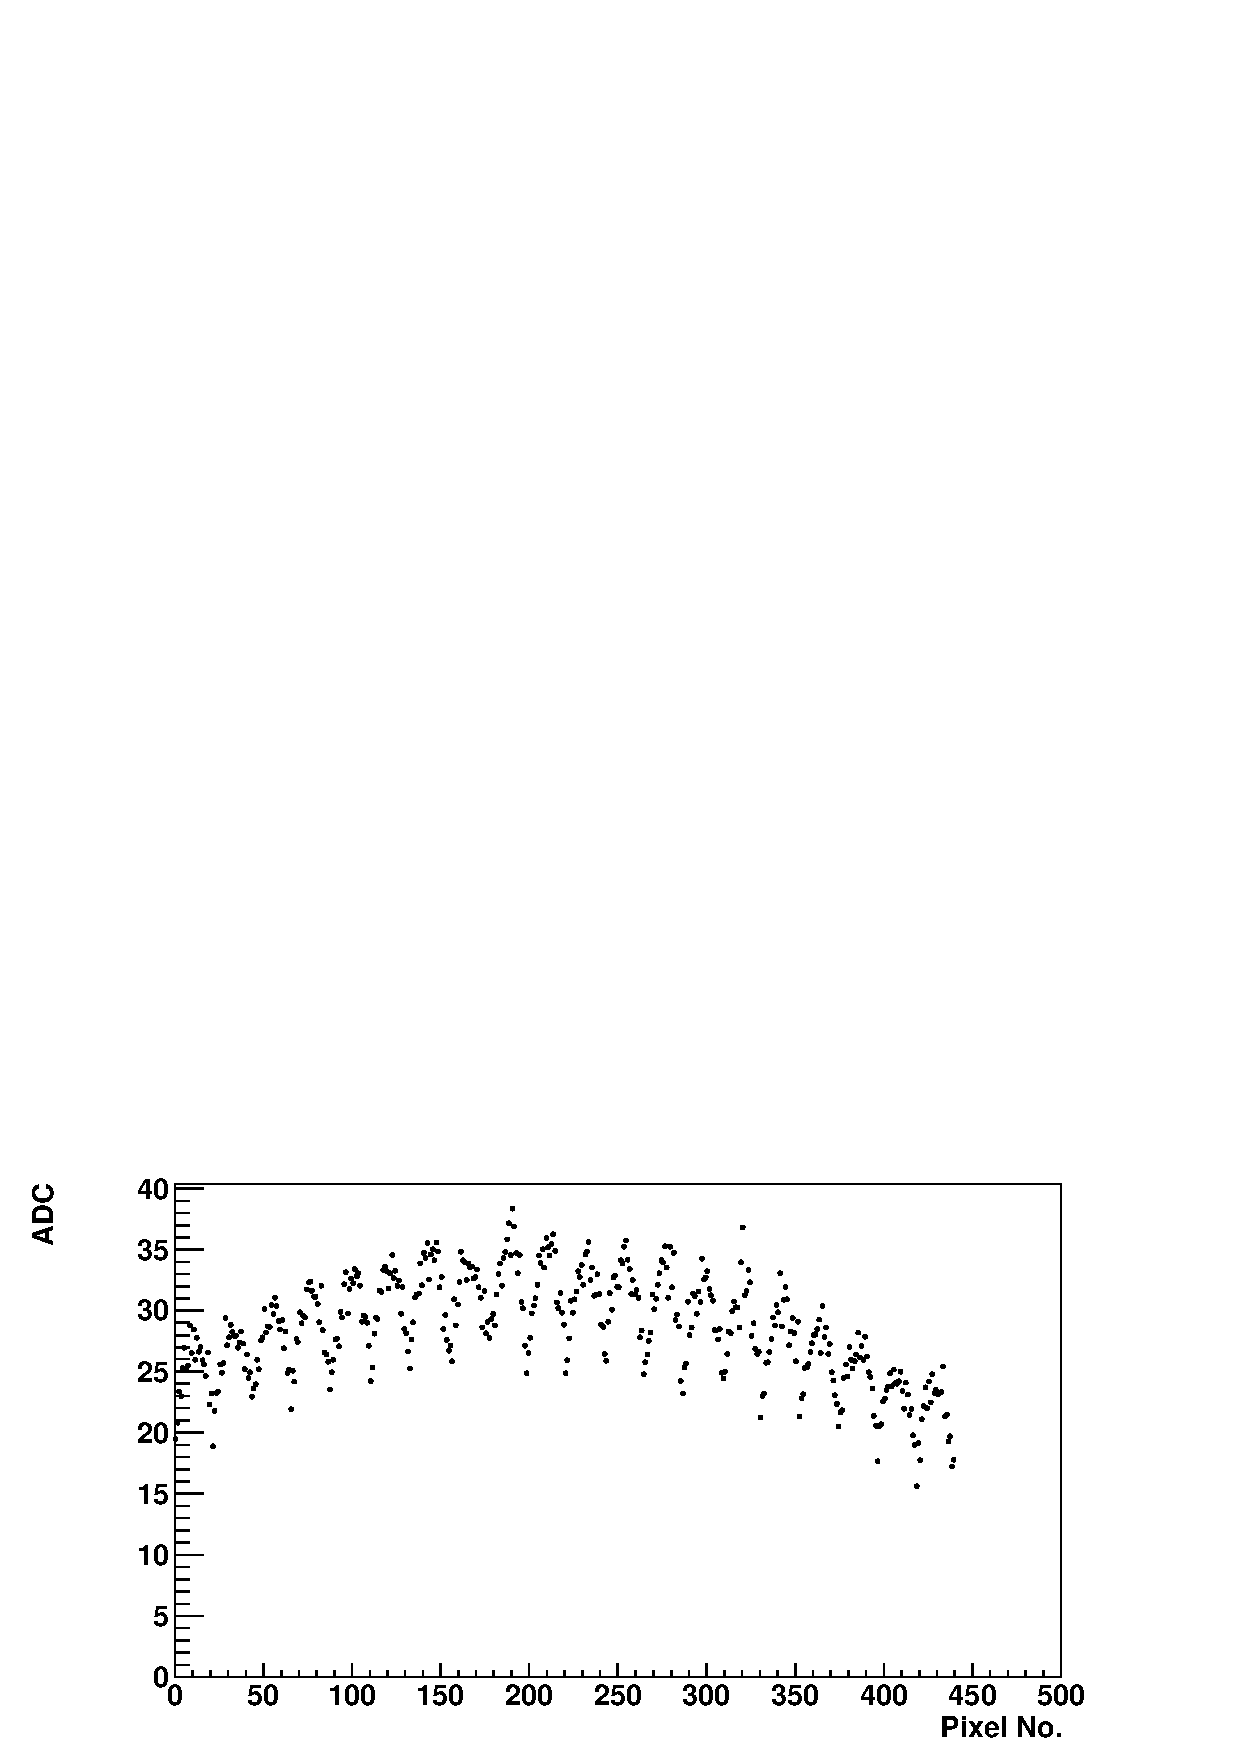
\includegraphics[width=\textwidth]{chapters/graphs/GainVarsMeas/LL_m04_2016-06-11/Set0and2/meanHist_LowHV_Pairs_set0and2.pdf}
\caption{} \label{fig:CalAMeanADC_Pairs}
\end{figure}

\begin{figure} % Variance Plot
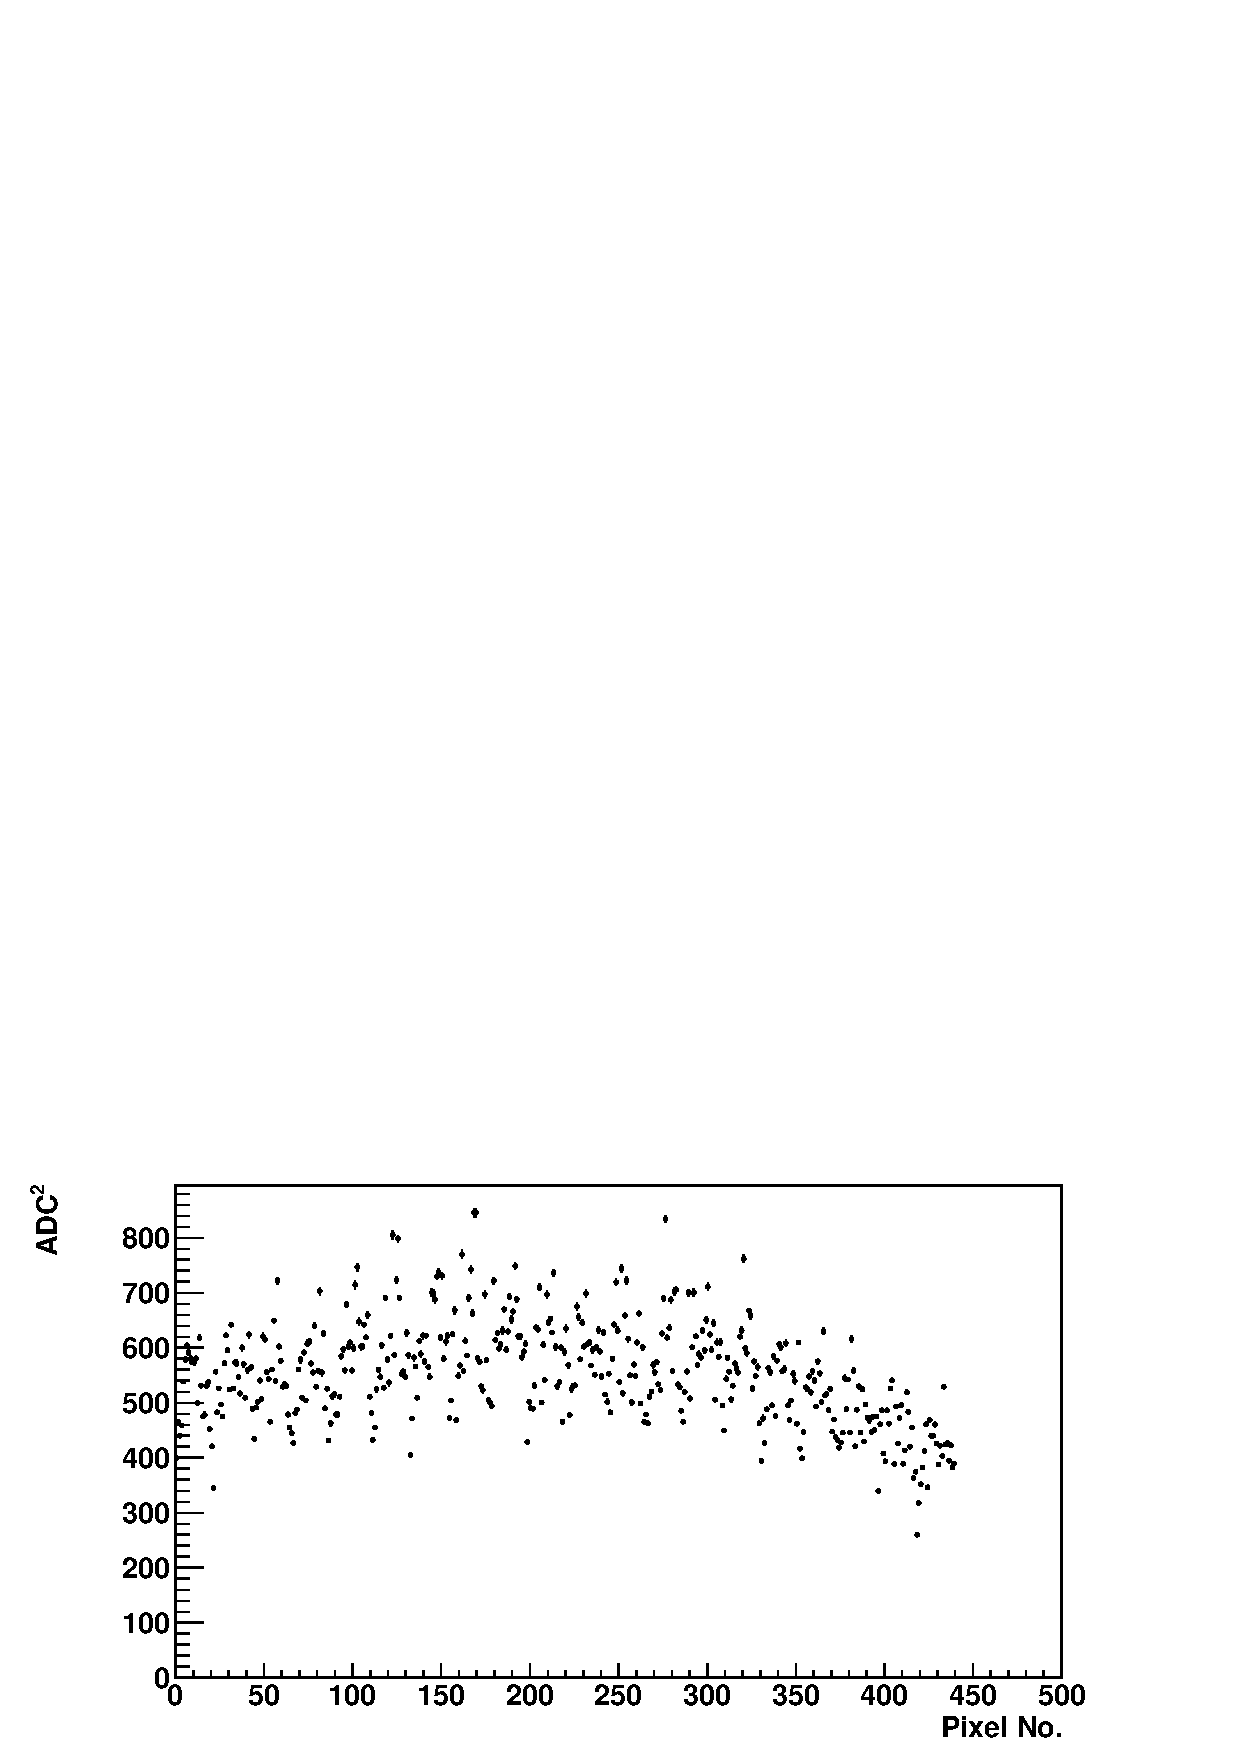
\includegraphics[width=\textwidth]{chapters/graphs/GainVarsMeas/LL_m04_2016-06-11/Set0and2/varianceHist_StandHV_Pairs_set0and2.pdf}
\caption{}
\vspace{3mm}
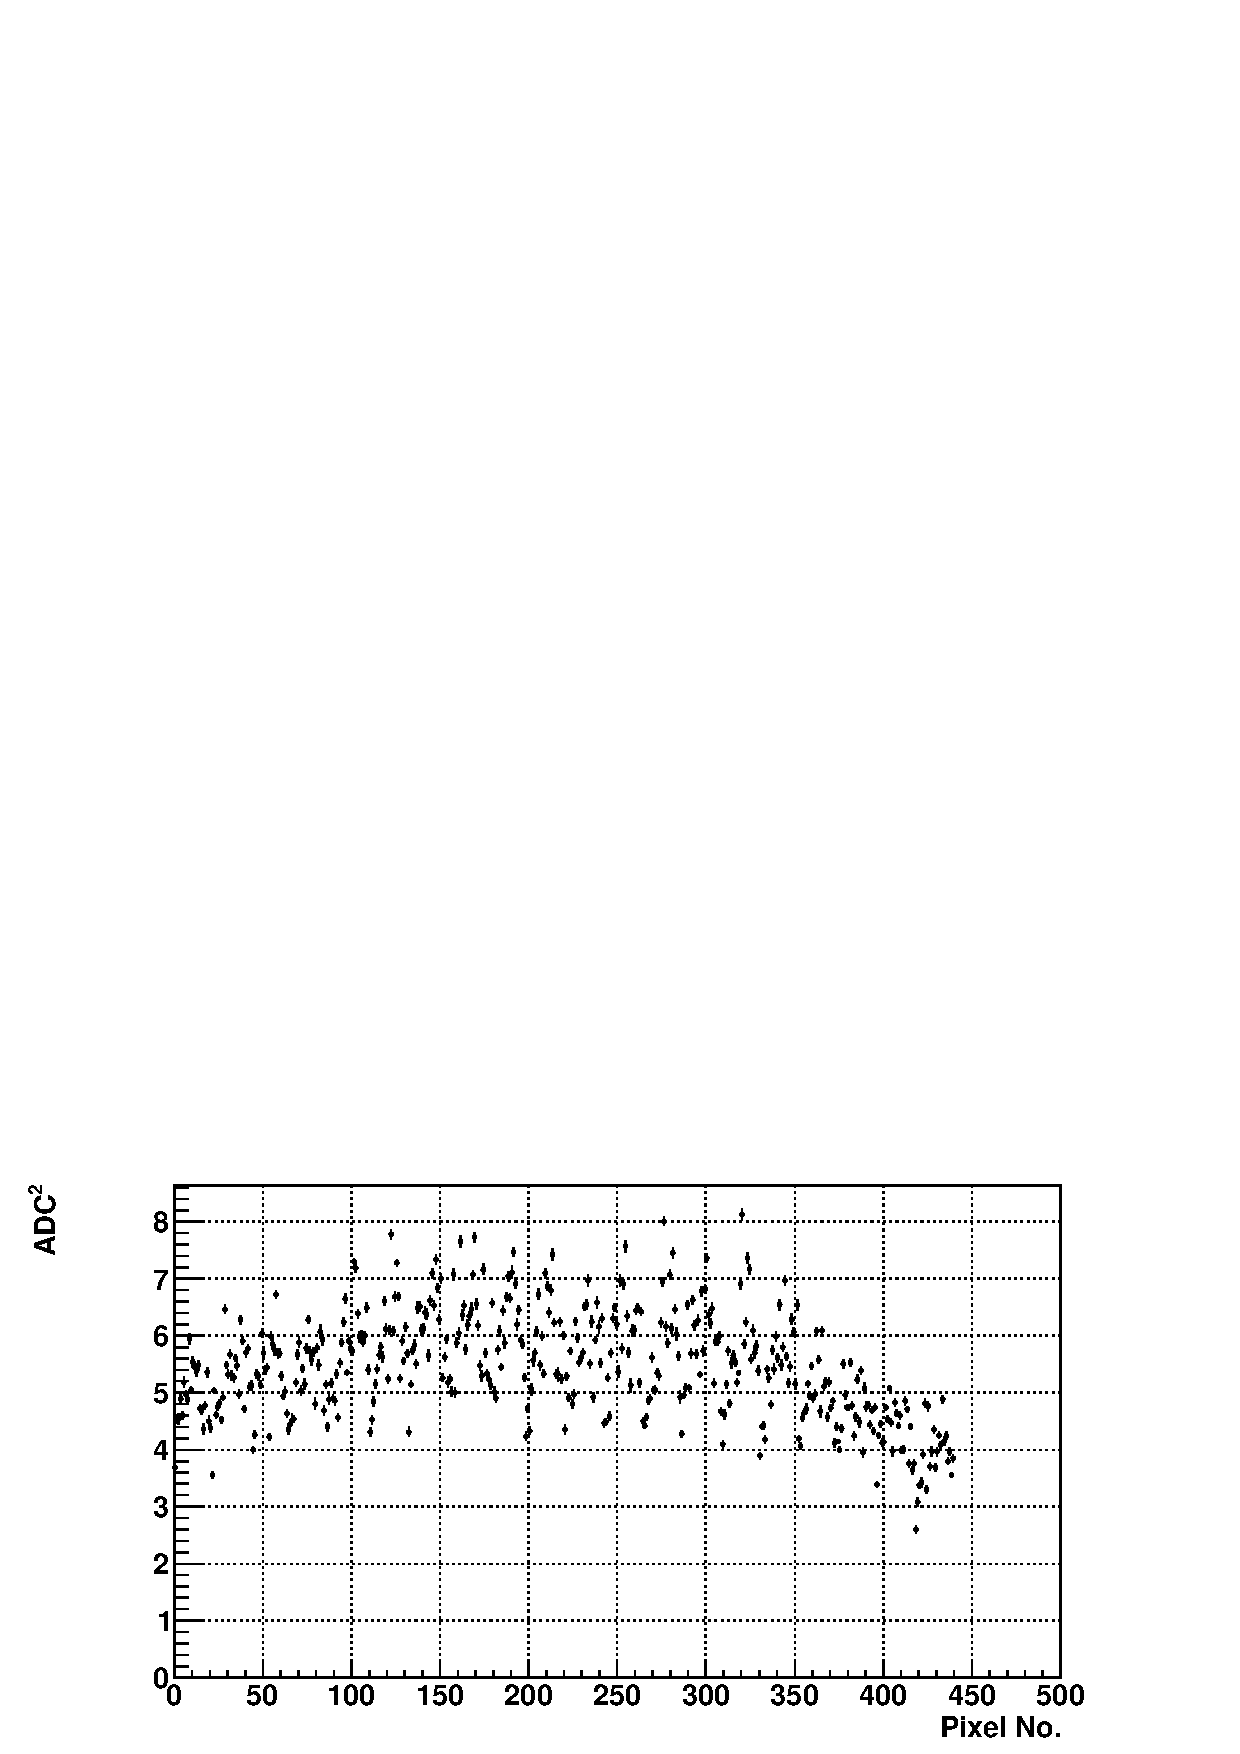
\includegraphics[width=\textwidth]{chapters/graphs/GainVarsMeas/LL_m04_2016-06-11/Set0and2/varianceHist_LowHV_Pairs_set0and2.pdf}
\caption{} \label{fig:CalAVarsADC_Pairs}
\end{figure}

\begin{figure} % Gain Variance Plot
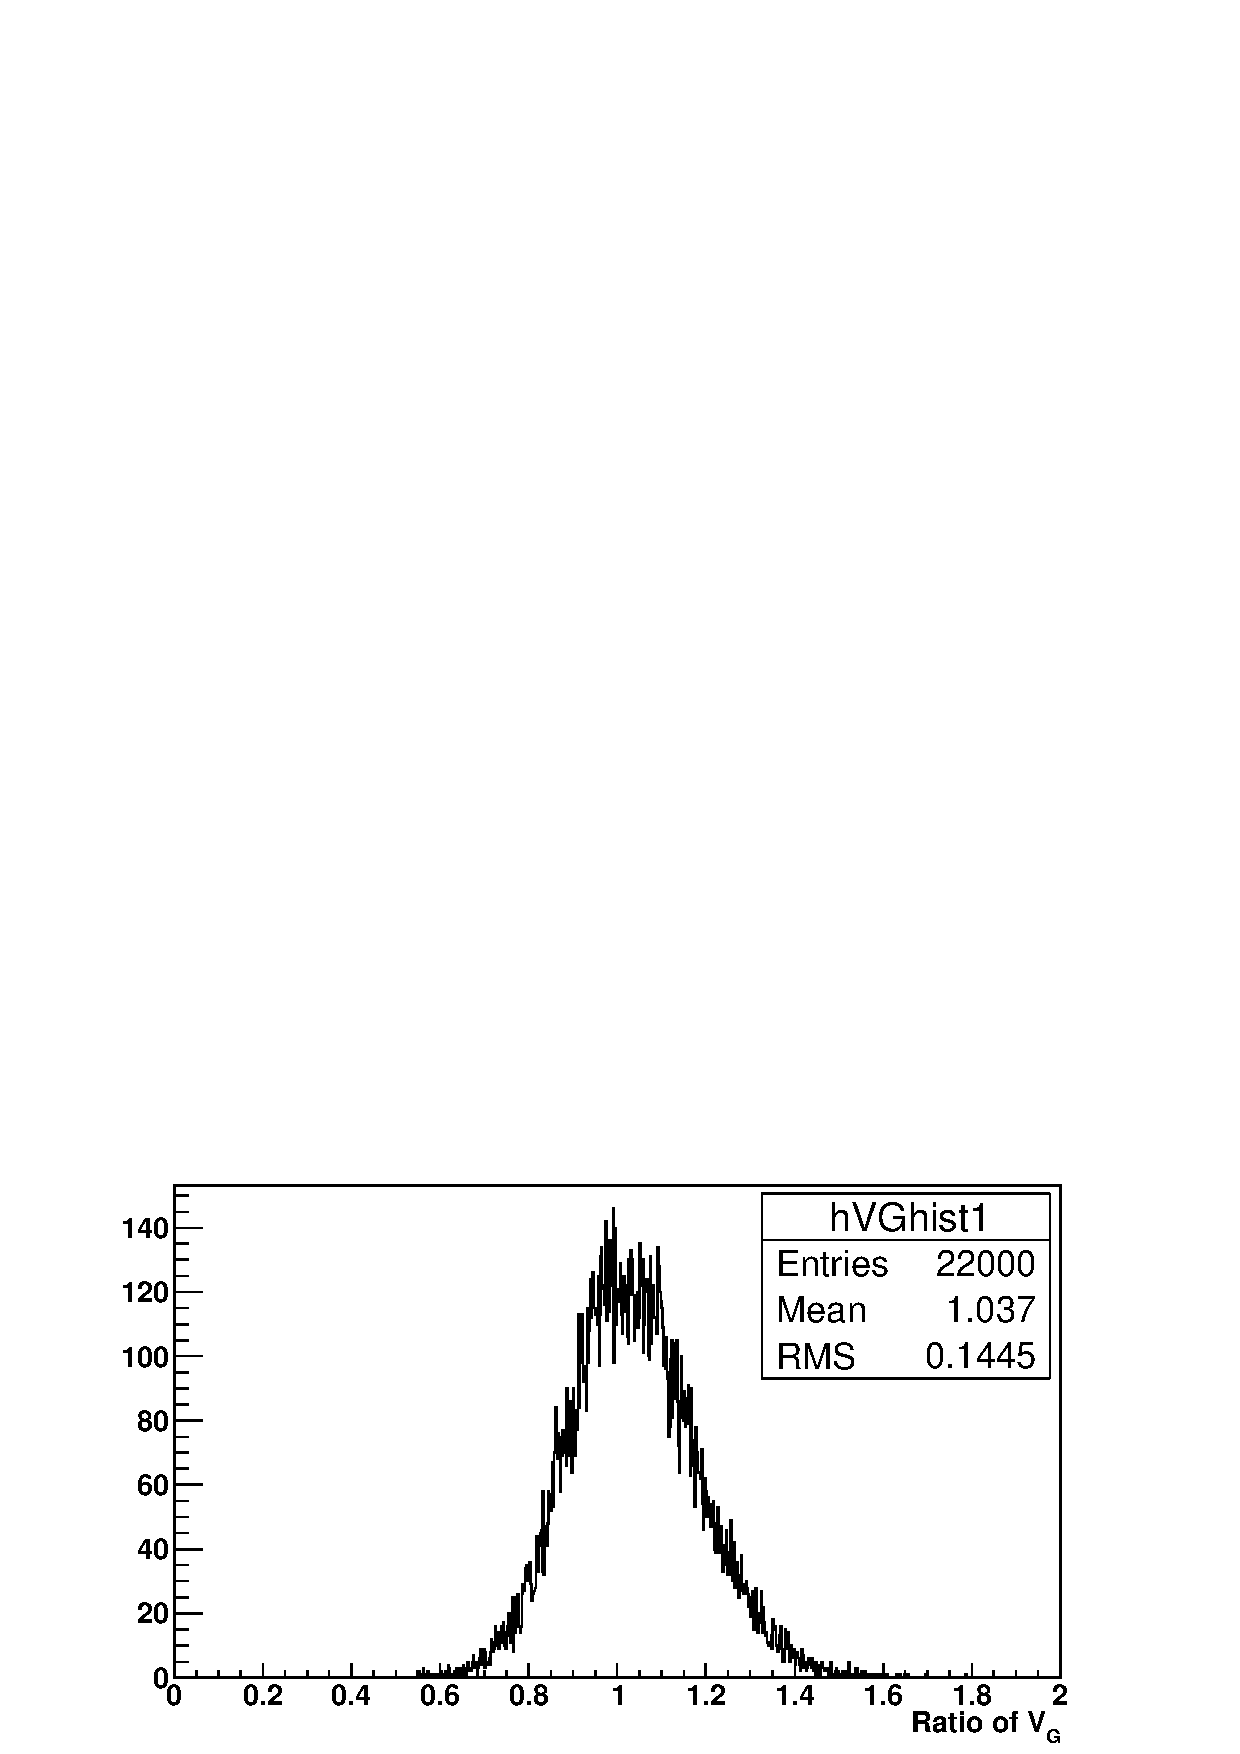
\includegraphics[width=\textwidth]{chapters/graphs/GainVarsMeas/LL_m04_2016-06-11/Set0and2/GainVairanceHist_Pairs.pdf}
\caption{}
\vspace{3mm}
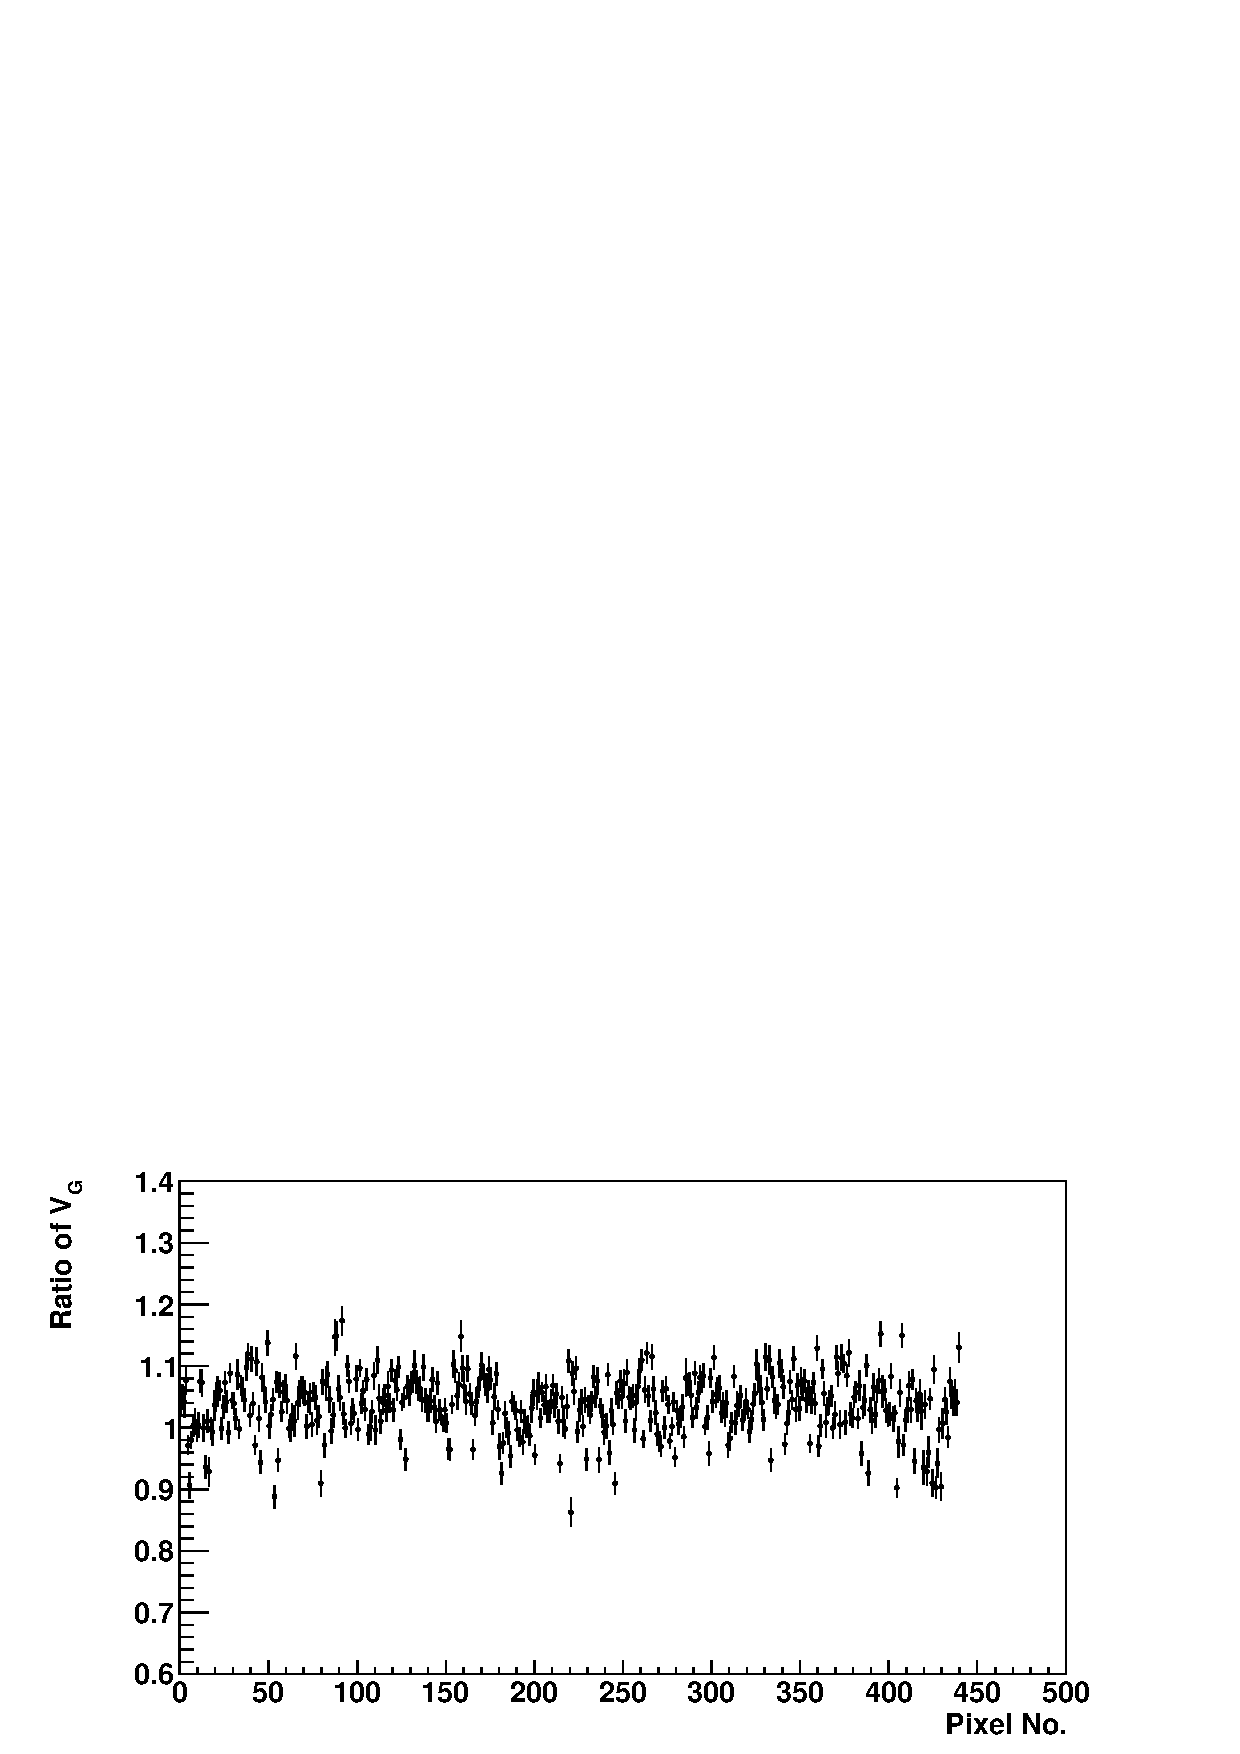
\includegraphics[width=\textwidth]{chapters/graphs/GainVarsMeas/LL_m04_2016-06-11/Set0and2/GainVars_Vs_Pixel_GainVariance_Pairs_Set0and2.pdf}
\caption{}
\end{figure}

\section{Result of Averaging Sets of Traces Method}

\begin{figure} % Mean Plot
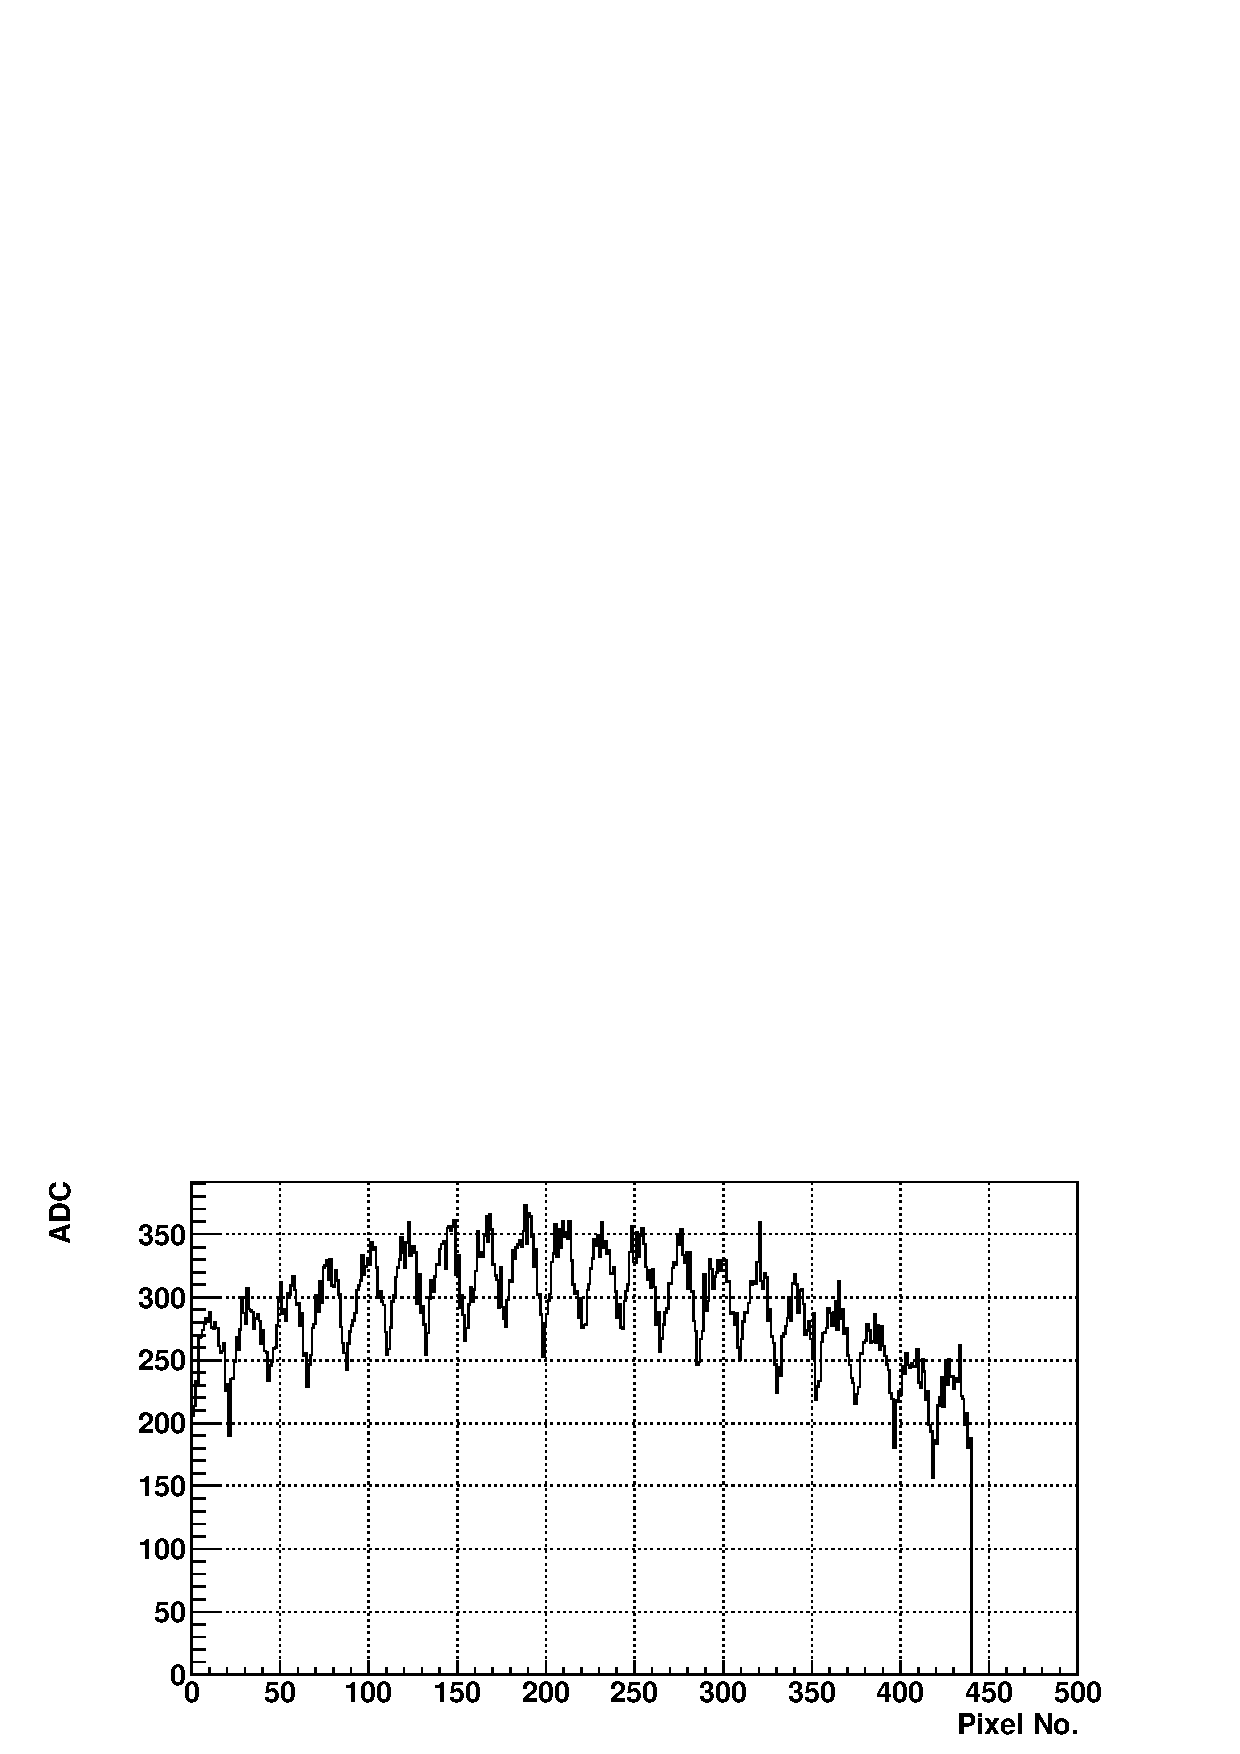
\includegraphics[width=\textwidth]{chapters/graphs/GainVarsMeas/LL_m04_2016-06-11/Set0and2/meanHist_StandHV_Average_set0and2.pdf}
\caption{}
\vspace{3mm}
\includegraphics[width=\textwidth]{chapters/graphs/GainVarsMeas/LL_m04_2016-06-11/Set0and2/meanHist_LowHV_Average_set0and2.pdf}
\caption{}
\end{figure}

\begin{figure} % Variance Plot
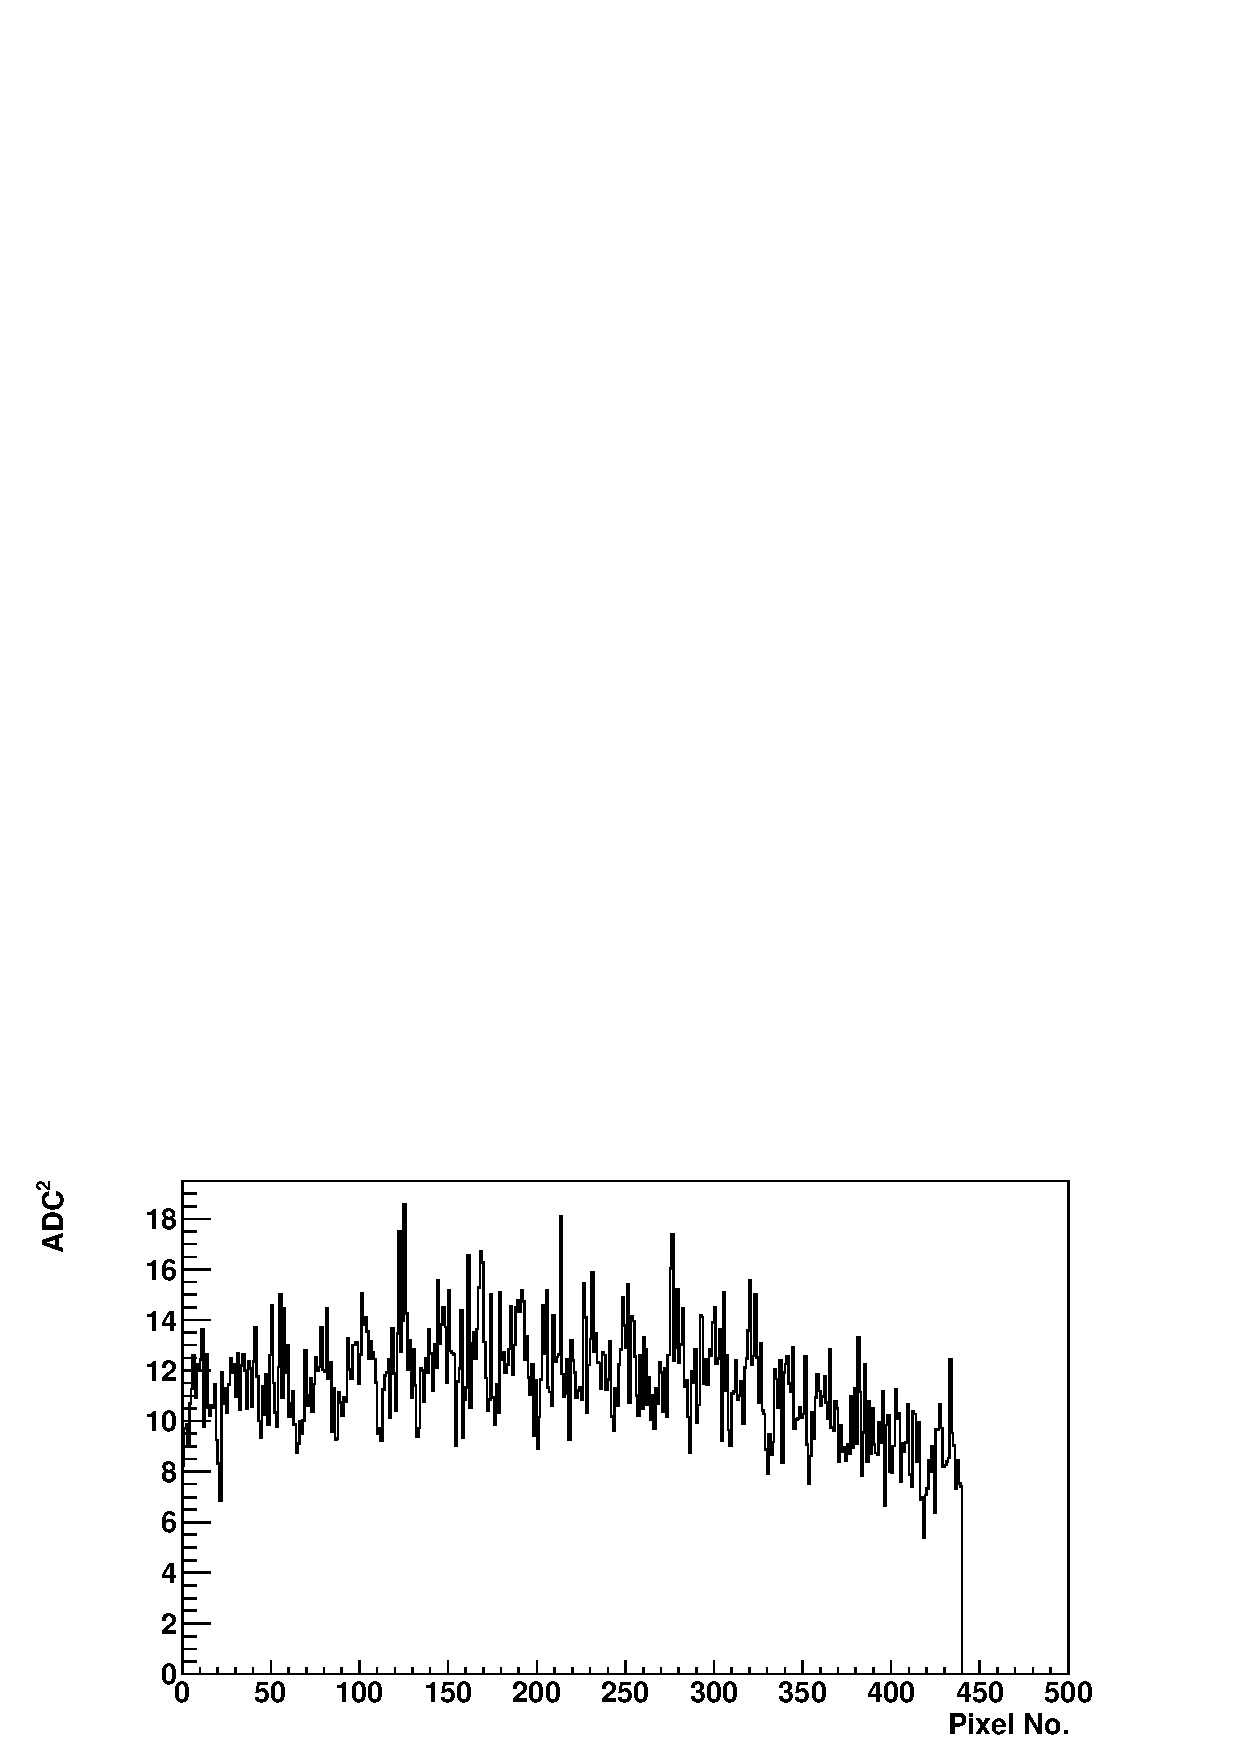
\includegraphics[width=\textwidth]{chapters/graphs/GainVarsMeas/LL_m04_2016-06-11/Set0and2/varianceHist_StandHV_Average_set0and2.pdf}
\caption{}
\vspace{3mm}
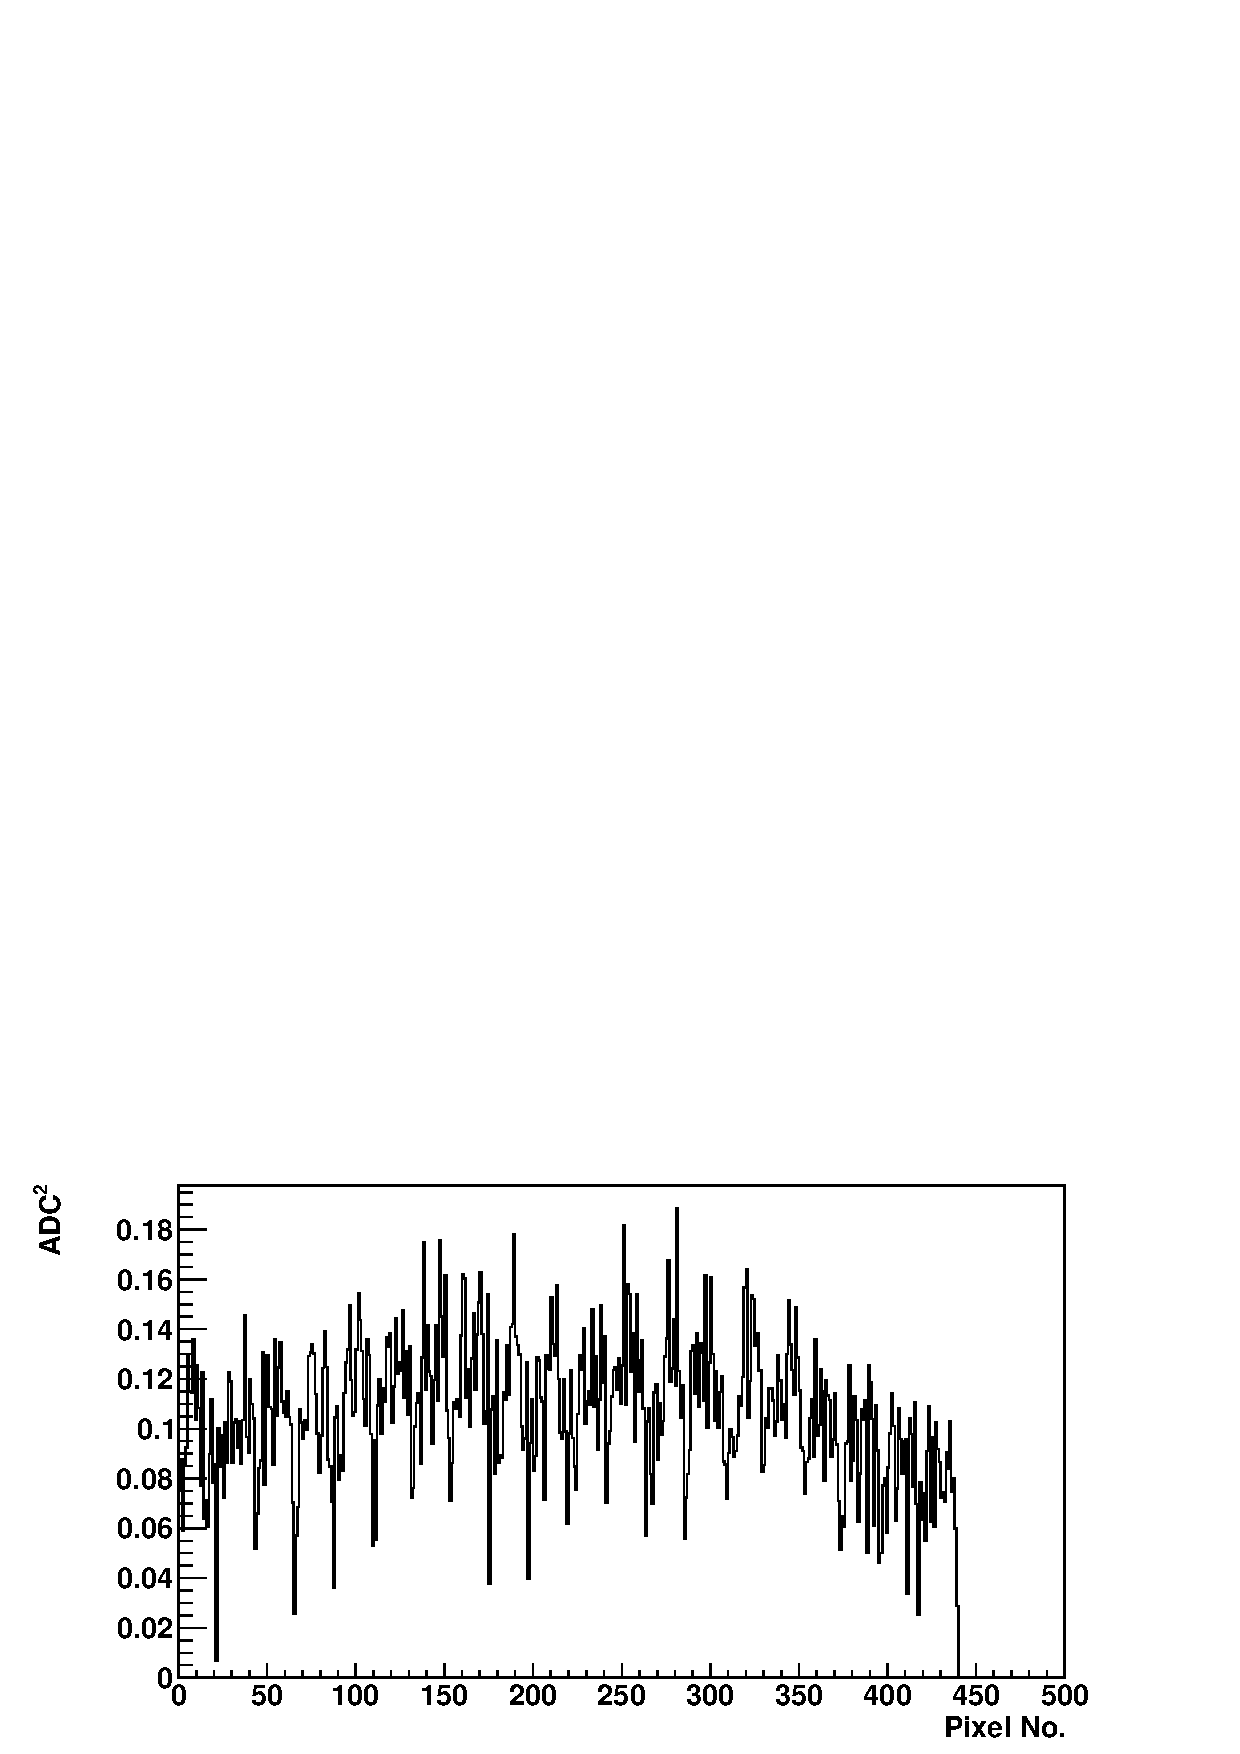
\includegraphics[width=\textwidth]{chapters/graphs/GainVarsMeas/LL_m04_2016-06-11/Set0and2/varianceHist_LowHV_Average_set0and2.pdf}
\caption{}
\end{figure}

\begin{figure} % Gain Variance Plot
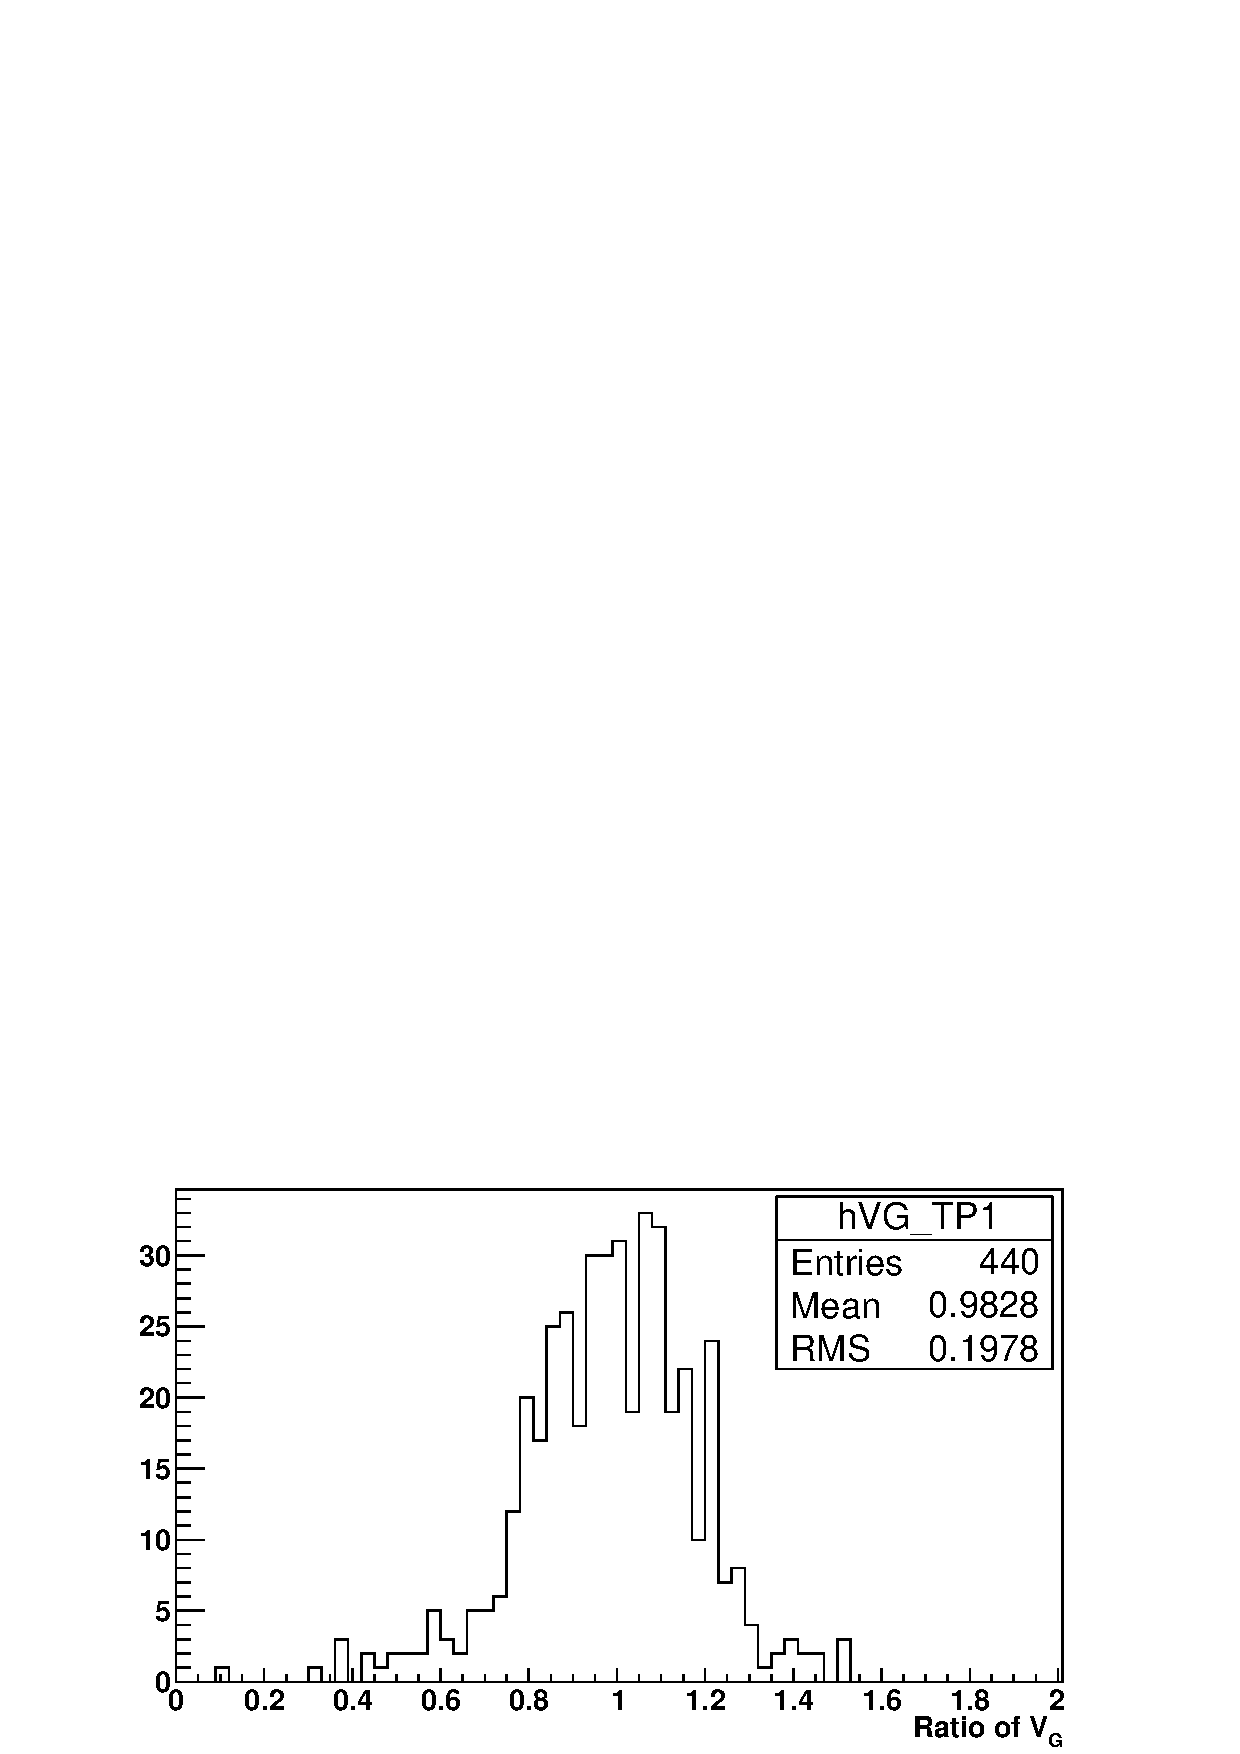
\includegraphics[width=\textwidth]{chapters/graphs/GainVarsMeas/LL_m04_2016-06-11/Set0and2/GainVairanceHist_Average_Method1.pdf}
\caption{}
\vspace{3mm}
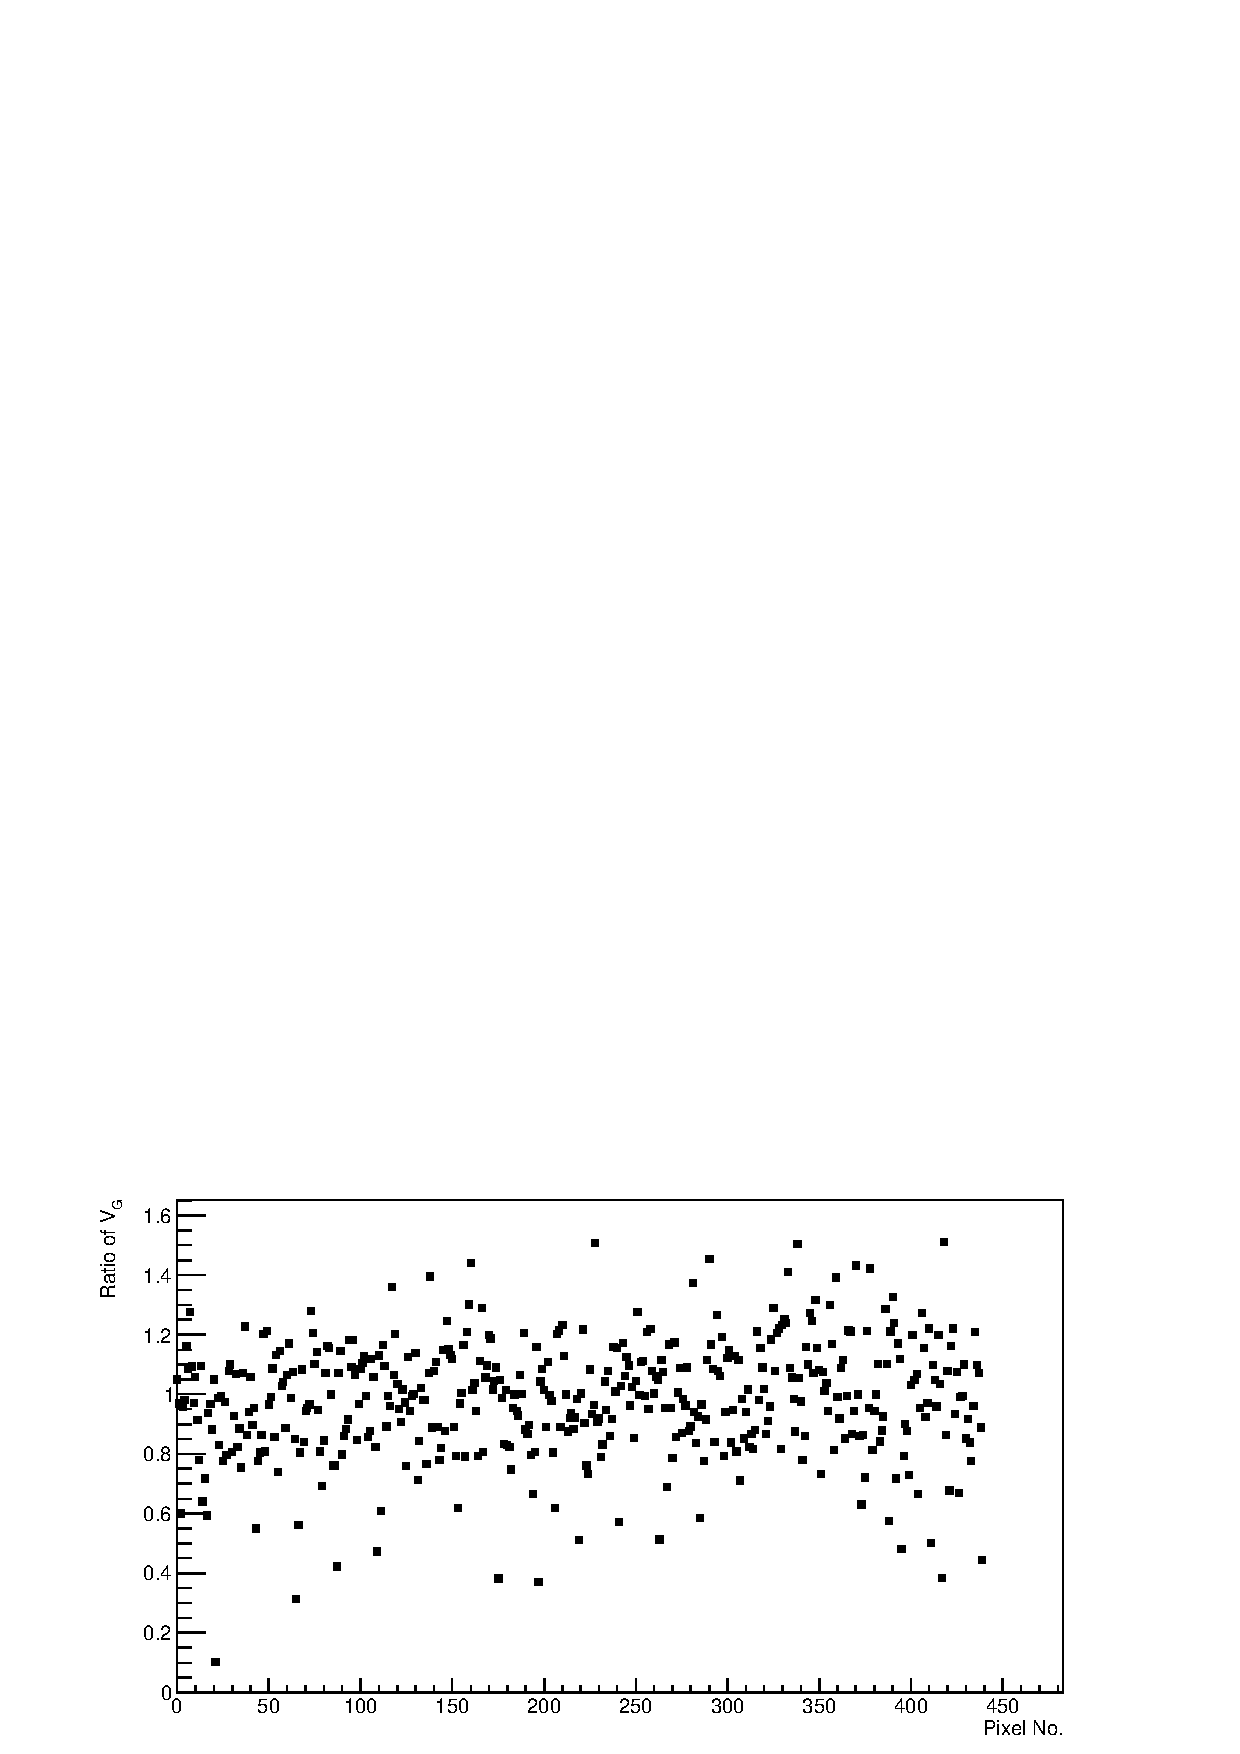
\includegraphics[width=\textwidth]{chapters/graphs/GainVarsMeas/LL_m04_2016-06-11/Set0and2/GainVars_Vs_Pixel_GainVariance_Average_Method1_Set0and2.pdf}
\caption{}
\end{figure}

\section{Result of Averaging Sets of Traces Method with Least Trimmed Squares}

\begin{figure}% Signal Chi2
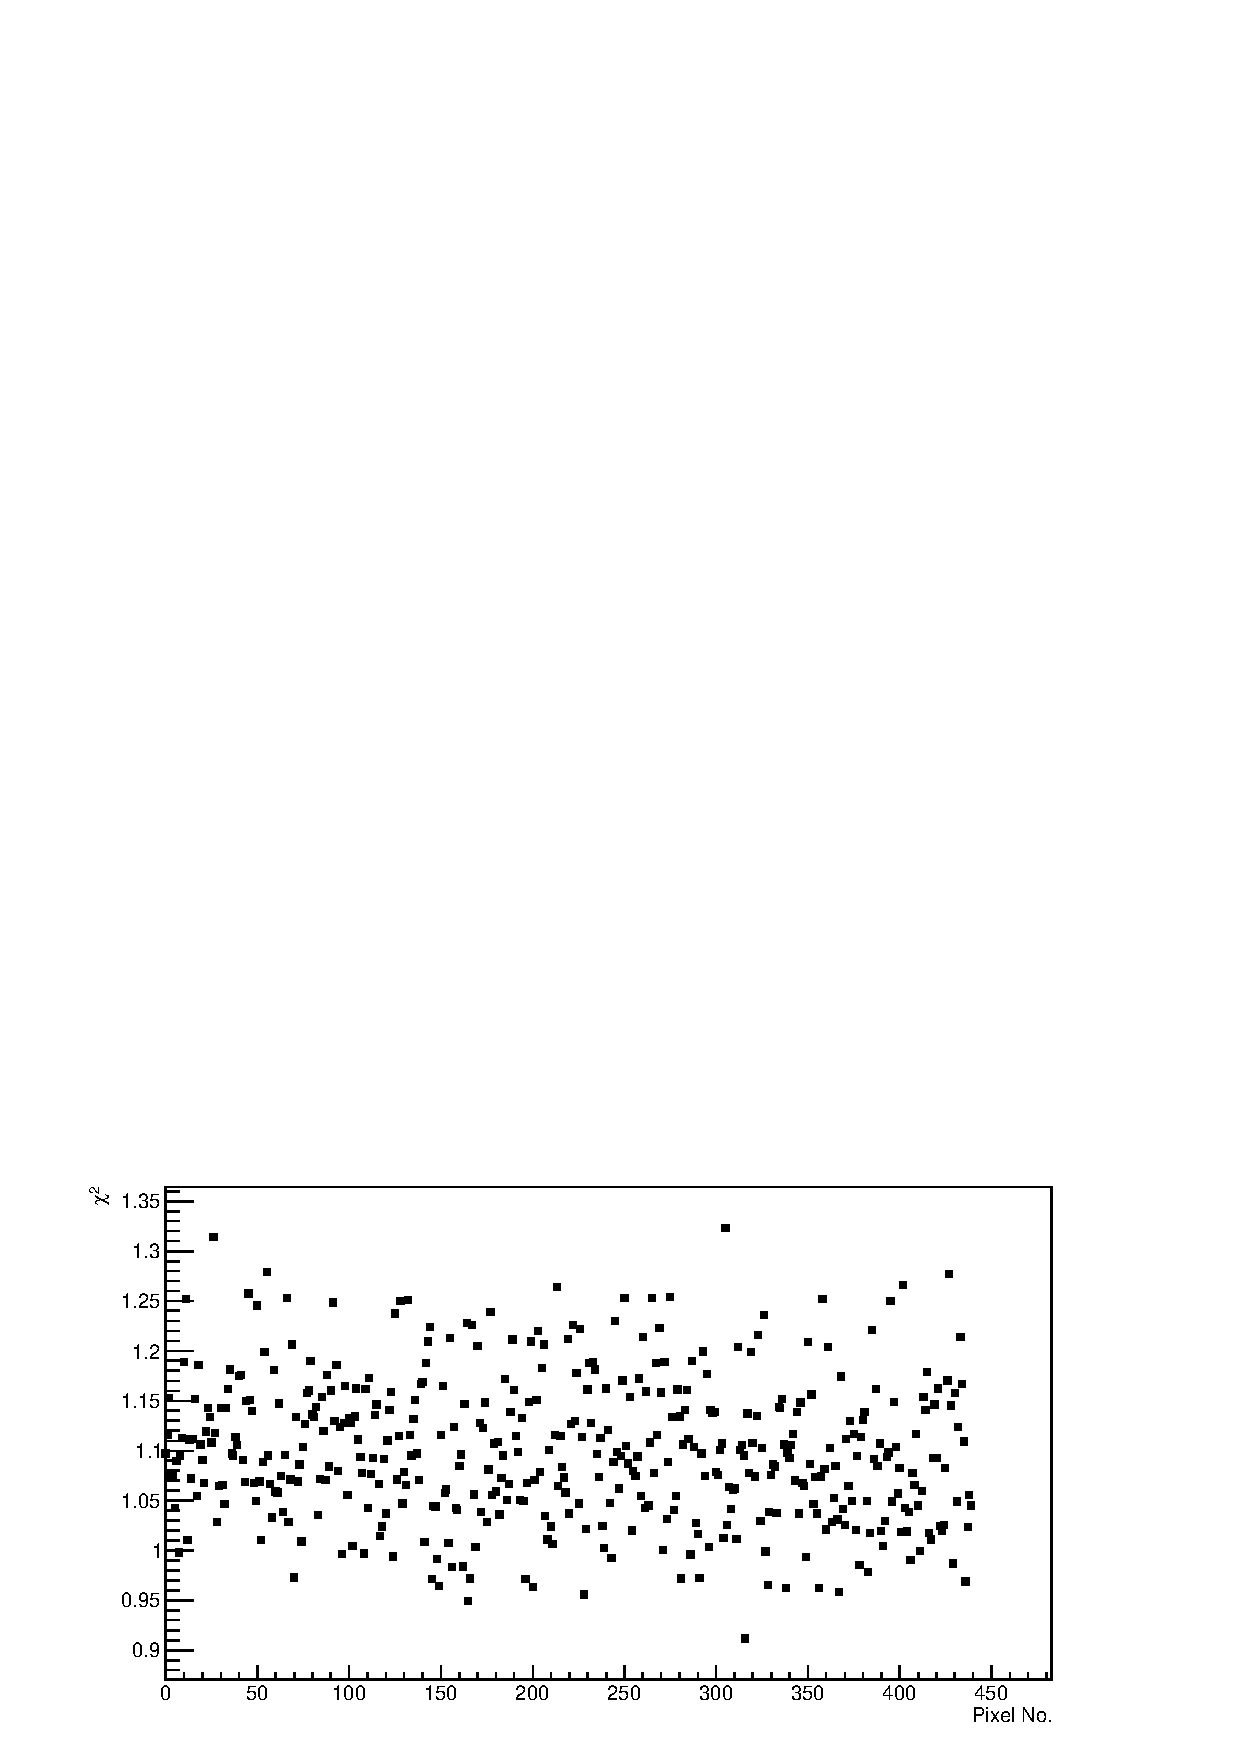
\includegraphics[width=\textwidth]{chapters/graphs/GainVarsMeas/LL_m04_2016-06-11/Set0and2/Chi2_AverageMethod_Signal_StandHV.pdf}
\caption{}
\vspace{3mm}
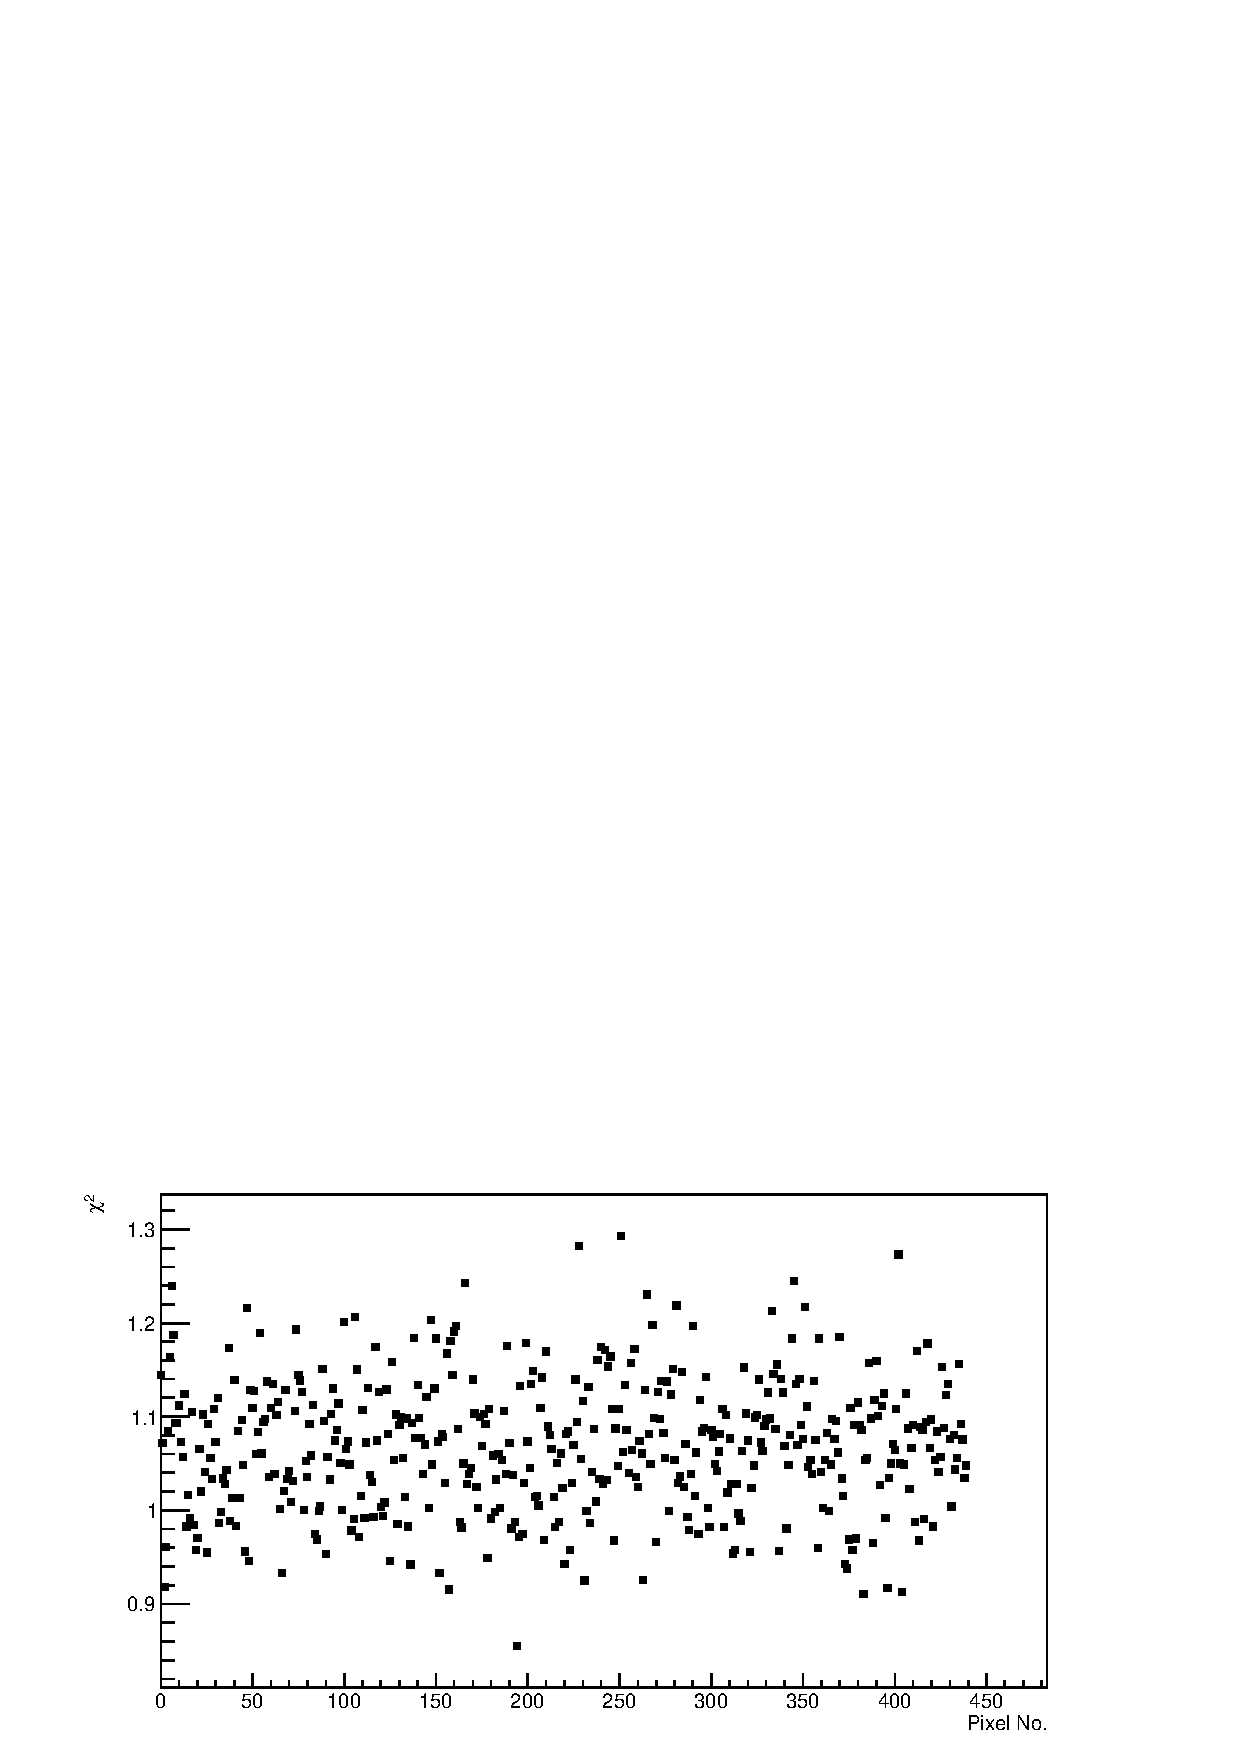
\includegraphics[width=\textwidth]{chapters/graphs/GainVarsMeas/LL_m04_2016-06-11/Set0and2/Chi2_AverageMethod_Signal_LowHV.pdf}
\caption{}
\end{figure}

\begin{figure}% Noise Chi2
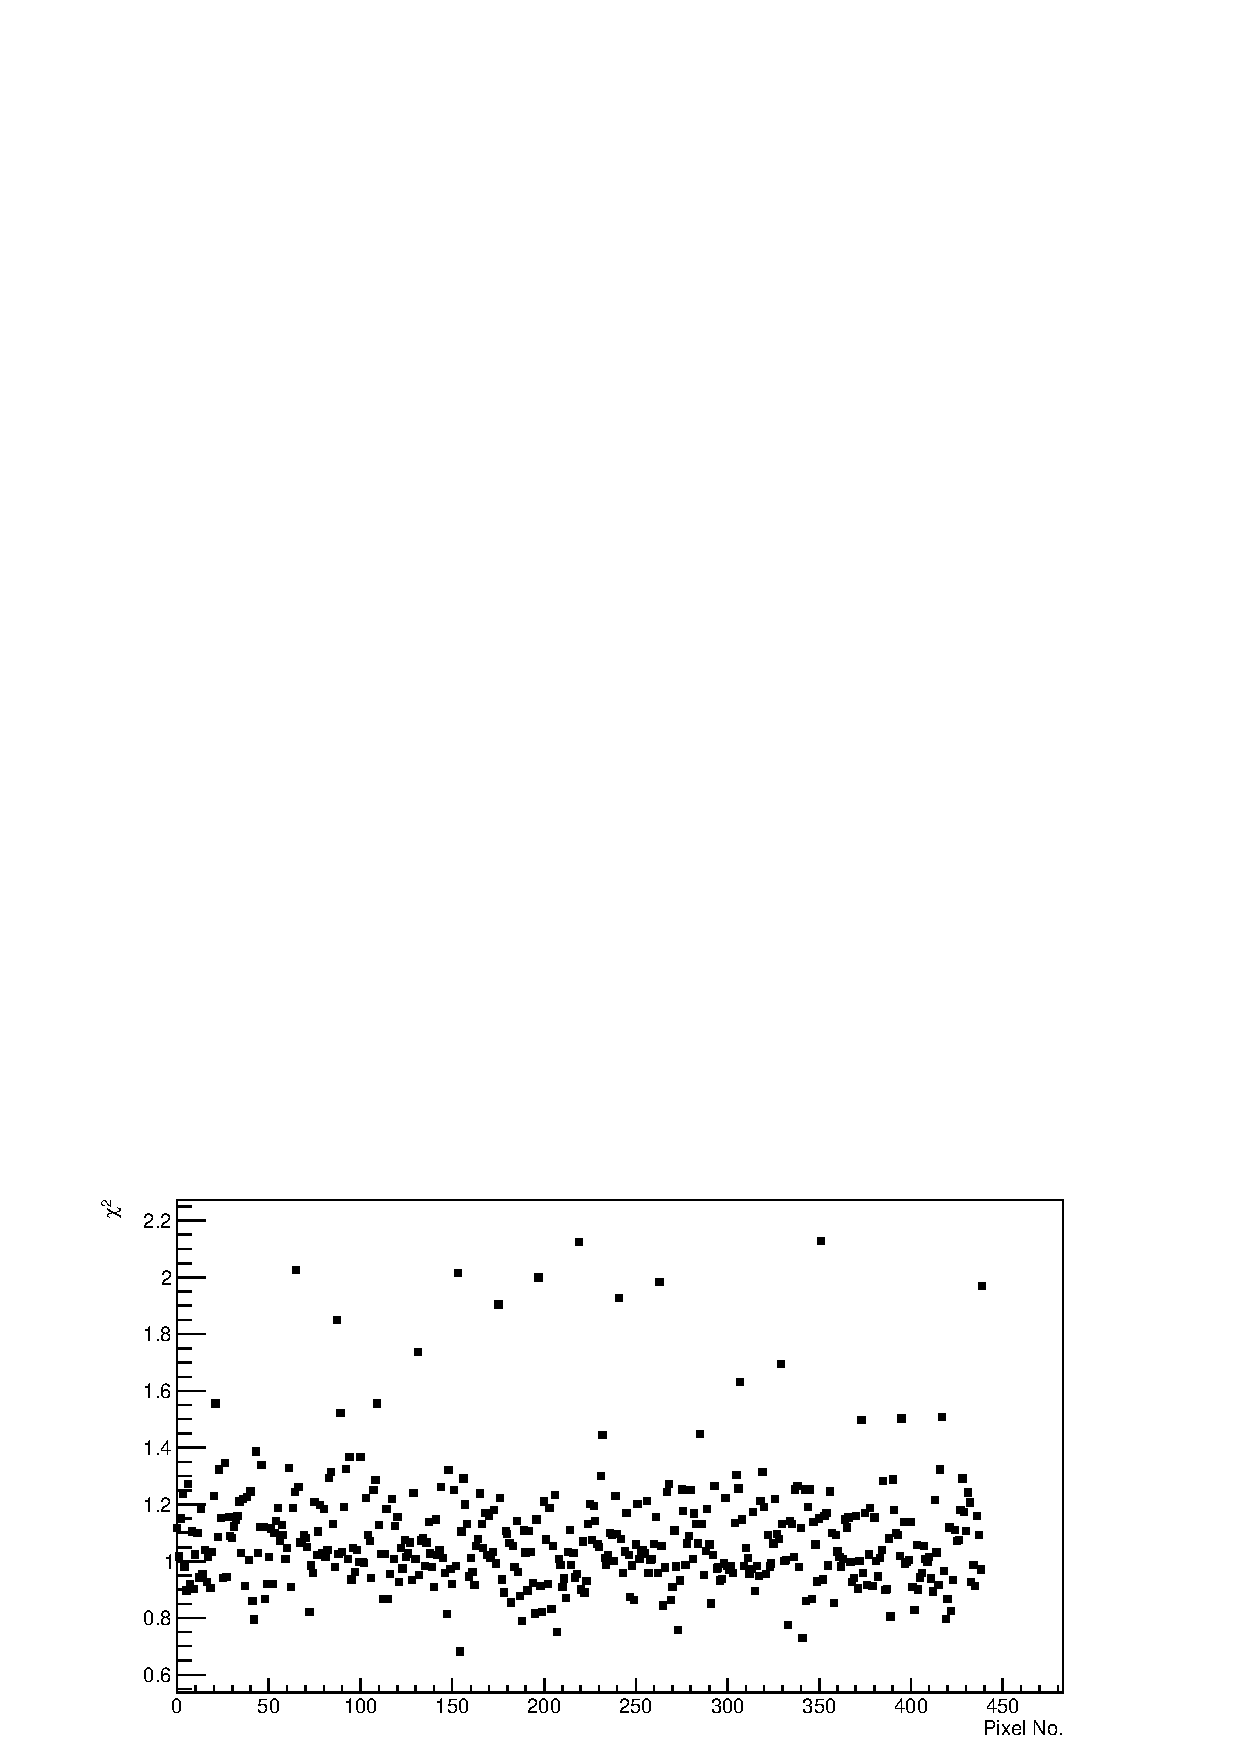
\includegraphics[width=\textwidth]{chapters/graphs/GainVarsMeas/LL_m04_2016-06-11/Set0and2/Chi2_AverageMethod_Noise_StandHV.pdf}
\caption{}
\vspace{3mm}
\includegraphics[width=\textwidth]{chapters/graphs/GainVarsMeas/LL_m04_2016-06-11/Set0and2/Chi2_AverageMethod_Noise_LowHV.pdf}
\caption{}
\end{figure}


\begin{figure} % Gain Variance Plot
\includegraphics[width=\textwidth]{chapters/graphs/GainVarsMeas/LL_m04_2016-06-11/Set0and2/GainVairanceHist_Average_LTS.pdf}
\caption{}
\vspace{3mm}
\includegraphics[width=\textwidth]{chapters/graphs/GainVarsMeas/LL_m04_2016-06-11/Set0and2/GainVars_Vs_Pixel_GainVariance_AverageLTS_Set0and2.pdf}
\caption{}
\end{figure}

\section{Result of Averaging Sets of Traces Method using Noise Distribution}

\begin{figure} % Gain Variance Plot
\includegraphics[width=\textwidth]{chapters/graphs/GainVarsMeas/LL_m04_2016-06-11/Set0and2/GainVairanceHist_Average_Method2.pdf}
\caption{}
\vspace{3mm}
\includegraphics[width=\textwidth]{chapters/graphs/GainVarsMeas/LL_m04_2016-06-11/Set0and2/GainVars_Vs_Pixel_GainVariance_Average_Method2_Set0and2.pdf}
\caption{}
\end{figure}

\section{Attempts to measure Gain Variance directly in the Lab}
\chapter{Laboratory Simulation of FD shift}\label{Ch:LabPMTshift}

Laboratory Simulation of FD shift under differing NSB levels.
\begin{itemize}
\item Measurements for both 900V and 600V (900V used as baseline)
\item Different length shifts
\item Changing NSB
\item measuring how the relevant Gain changes throughout a run
\end{itemize}
\chapter[Evaluation of Cloud Camera Cuts]{\centering Evaluation of Cloud Camera Cuts \\}\label{Ch:CloudCuts}

First look into the effectiveness of the Cloud Camera cuts on PAO Golen Hybrid data.
\begin{itemize}
\item Are we being too conservative?
\item Effects on Xmax, Zenith and Rp distributions
\end{itemize}  

\chapter[Conclusion]{\centering Conclusion \\} \label{Ch:Conclusion}
  

\section{Future Work}



% Other plots and stuff

\begin{appendices}
%\input{appendix/}
%\input{appendix/}
%\input{appendix/}
%\input{appendix/}
\end{appendices}

\bibliographystyle{ieeetr}
\bibliography{PhD_PaperBiblography}

\end{document}